% Contents from body/page-307.tex.
\BookMark{0}{IV  Curves}{p-307}
\ChapterSheet{307}{293}{}{%
\vspace*{22pt}
\noindent{\large\bfseries IV}\par\vspace{3pt}
\hrule
\vspace{6pt}
\noindent{\Large\bfseries Curves}\par
\vspace{166pt}
\noindent In this chapter we apply the techniques we have learned earlier to study curves. But in fact, except for the proof of the Riemann--Roch theorem \Goto{result-IV-1.3}{(1.3)}, which uses Serre duality, we use very little of the fancy methods of schemes and cohomology. So if a reader is willing to accept the statement of the Riemann--Roch theorem, he can read this chapter at a much earlier stage of his study of algebraic geometry. That may not be a bad idea, pedagogically, because in that way he will see some applications of the general theory, and in particular will gain some respect for the significance of the Riemann--Roch theorem. In contrast, the proof of the Riemann--Roch theorem is not very enlightening.

After reviewing what is needed from the earlier part of the book in \Goto{sec-IV-1}{\S1}, we study in \S\Goto{sec-IV-2}{2}, \Goto{sec-IV-3}{3} various ways of representing a curve explicitly. One way is to represent the curve as a branched covering of $\Proj^1$. So in \Goto{sec-IV-2}{\S2} we make a general study of one curve as a branched covering of another. The central result here is Hurwitz's theorem \Goto{result-IV-2.4}{(2.4)} which compares the canonical divisors on the two curves.

In \Goto{sec-IV-3}{\S3} we give two other ways of representing a curve. We show that any nonsingular projective curve can be embedded in $\Proj^3$, and it can be mapped birationally into $\Proj^2$ in such a way that the image has only nodes for singularities. The proof of the latter theorem has an interesting extra twist in characteristic $p>0$.

In \Goto{sec-IV-4}{\S4} we discuss the special case of curves of genus $1$, called elliptic curves. This is a whole subject in itself, quite independent of the rest of the chapter. We have space for only a brief glimpse of some aspects of this fascinating theory.

In \S\Goto{sec-IV-5}{5}, \Goto{sec-IV-6}{6} we discuss the canonical embedding, and some classification questions, both for abstract curves and for curves in $\Proj^3$.
}
% Contents from body/page-308.tex.
\BookMark{1}{4.1  Riemann\textendash{}Roch Theorem}{sec-IV-1}
\ChapterSheet{308}{294}{\Goto{p-307}{IV\quad Curves}}{%
\vspace*{22pt}
\noindent\hypertarget{sec-IV-1}{}{\large\bfseries 1\quad Riemann--Roch Theorem}\par\nobreak\vspace{8pt}
\noindent In this chapter we will use the word \emph{curve} to mean a complete, nonsingular curve over an algebraically closed field $k$. In other words (II, \Goto{sec-II-6}{\S6}), a curve is an integral scheme of dimension $1$, proper over $k$, all of whose local rings are regular. Such a curve is necessarily projective (II, \Goto{result-II-6.7}{6.7}). If we want to consider a more general kind of curve, we will use the word \textquotedblleft{}scheme,\textquotedblright{} appropriately qualified, e.g., \textquotedblleft{}an integral scheme of dimension $1$ of finite type over $k$.\textquotedblright{} We will use the word \emph{point} to mean a closed point, unless we specify the \emph{generic point}.

We begin by reviewing some of the concepts introduced earlier in the book, which we will use in our study of curves.

The most important single invariant of a curve is its genus. There are several ways of defining it, all equivalent. For a curve $X$ in projective space, we have the \emph{arithmetic genus} $p_a(X)$, defined as $1-P_X(0)$, where $P_X$ is the Hilbert polynomial of $X$ (I, Ex.~\Goto{ex-I-7.2}{7.2}). On the other hand, we have the \emph{geometric genus} $p_g(X)$, defined as $\dim_k\Gamma(X,\omega_X)$, where $\omega_X$ is the canonical sheaf (II, \Goto{result-II-8.18.2}{8.18.2}).

\medskip
\noindent\hypertarget{result-IV-1.1}{}\textbf{Proposition 1.1.} \emph{If $X$ is a curve, then}
\[
p_a(X)=p_g(X)=\dim_k H^1(X,\mathcal O_X),
\]
\emph{so we call this number simply the genus of $X$, and denote it by $g$.}

\smallskip
\noindent\textsc{Proof.} The equality $p_a(X)=\dim H^1(X,\mathcal O_X)$ has been shown in (III, Ex.~\Goto{ex-III-5.3}{5.3}). The equality $p_g=\dim H^1(X,\mathcal O_X)$ is a consequence of Serre duality (III, \Goto{result-III-7.12.2}{7.12.2}).

\medskip
\noindent\hypertarget{result-IV-1.1.1}{}\textbf{Remark 1.1.1.} From $g=p_g$, we see that the genus of a curve is always nonnegative. Conversely, for any $g\geq0$, there exist curves of genus $g$. For example, take a divisor of type $(g+1,2)$ on a nonsingular quadric surface. There exist such divisors which are irreducible and nonsingular, and they have $p_a=g$ (III, Ex.~\Goto{ex-III-5.6}{5.6}).

\medskip
A \emph{(Weil) divisor} on the curve $X$ is an element of the free abelian group generated by the set of points of $X$ (II, \Goto{sec-II-6}{\S6}). We write a divisor as $D=\sum n_iP_i$ with $n_i\in\mathbf Z$. Its \emph{degree} is $\sum n_i$. Two divisors are \emph{linearly equivalent} if their difference is the divisor of a rational function. We have seen that the degree of a divisor depends only on its linear equivalence class (II, \Goto{result-II-6.10}{6.10}). Since $X$ is nonsingular, for every divisor $D$ we have an associated invertible sheaf $\mathcal L(D)$, and the correspondence $D\mapsto\mathcal L(D)$ gives an isomorphism of the group $\operatorname{Cl}(X)$ of divisors modulo linear equivalence with the group $\operatorname{Pic}X$ of invertible sheaves modulo isomorphism (II, \Goto{result-II-6.16}{6.16}).

A divisor $D=\sum n_iP_i$ on $X$ is \emph{effective} if all $n_i\geq0$. The set of all effective divisors linearly equivalent to a given divisor $D$ is called a \emph{complete linear}
}
% Contents from body/page-309.tex.
\ChapterSheet{309}{295}{\Goto{sec-IV-1}{1\quad Riemann--Roch Theorem}}{%
\emph{system} (II, \Goto{sec-II-7}{\S7}) and is denoted by $|D|$. The elements of $|D|$ are in one-to-one correspondence with the space
\[
(H^0(X,\mathcal L(D))-\{0\})/k^*,
\]
so $|D|$ carries the structure of the set of closed points of a projective space (II, \Goto{result-II-7.7}{7.7}). We denote $\dim_k H^0(X,\mathcal L(D))$ by $l(D)$, so that the \emph{dimension} of $|D|$ is $l(D)-1$. The number $l(D)$ is finite by (II, \Goto{result-II-5.19}{5.19}) or (III, \Goto{result-III-5.2}{5.2}).

As a consequence of this correspondence we have the following elementary, but useful, result.

\medskip
\noindent\hypertarget{result-IV-1.2}{}\textbf{Lemma 1.2.} \emph{Let $D$ be a divisor on a curve $X$. Then if $l(D)\ne0$, we must have $\deg D\geq0$. Furthermore, if $l(D)\ne0$ and $\deg D=0$, we must have $D\sim0$, i.e., $\mathcal L(D)\cong\mathcal O_X$.}

\smallskip
\noindent\textsc{Proof.} If $l(D)\ne0$, then the complete linear system $|D|$ is nonempty. Hence $D$ is linearly equivalent to some effective divisor. Since the degree depends only on the linear equivalence class, and the degree of an effective divisor is nonnegative, we find $\deg D\geq0$. If $\deg D=0$, then $D$ is linearly equivalent to an effective divisor of degree $0$. But there is only one such, namely the zero divisor.

\medskip
We denote by $\Omega_{X/k}$, or simply $\Omega_X$, the sheaf of relative differentials of $X$ over $k$ (II, \Goto{sec-II-8}{\S8}). Since $X$ has dimension $1$, it is an invertible sheaf on $X$, and so is equal to the canonical sheaf $\omega_X$ on $X$. We call any divisor in the corresponding linear equivalence class a \emph{canonical divisor}, and denote it by $K$. (We also occasionally use the letter $K$ to denote the function field of $X$, but it should be clear from the context which meaning is intended.)

\medskip
\noindent\hypertarget{result-IV-1.3}{}\textbf{Theorem 1.3} (Riemann--Roch). \emph{Let $D$ be a divisor on a curve $X$ of genus $g$. Then}
\[
l(D)-l(K-D)=\deg D+1-g.
\]

\smallskip
\noindent\textsc{Proof.} The divisor $K-D$ corresponds to the invertible sheaf $\omega_X\otimes\mathcal L(D)^\vee$. Since $X$ is projective (II, \Goto{result-II-6.7}{6.7}), we can apply Serre duality (III, \Goto{result-III-7.12.1}{7.12.1}) to conclude that the vector space $H^0(X,\omega_X\otimes\mathcal L(D)^\vee)$ is dual to $H^1(X,\mathcal L(D))$. Thus we have to show that for any $D$,
\[
\chi(\mathcal L(D))=\deg D+1-g,
\]
where for any coherent sheaf $\mathcal F$ on $X$, $\chi(\mathcal F)$ is the Euler characteristic
\[
\chi(\mathcal F)=\dim H^0(X,\mathcal F)-\dim H^1(X,\mathcal F).
\]
First we consider the case $D=0$. Then our formula says
\[
\dim H^0(X,\mathcal O_X)-\dim H^1(X,\mathcal O_X)=0+1-g.
\]
This is true, because $H^0(X,\mathcal O_X)=k$ for any projective variety (I, \Goto{result-I-3.4}{3.4}), and $\dim H^1(X,\mathcal O_X)=g$ by \Goto{result-IV-1.1}{(1.1)}.
}
% Contents from body/page-310.tex.
\ChapterSheet{310}{296}{\Goto{p-307}{IV\quad Curves}}{%
\indent Next, let $D$ be any divisor, and let $P$ be any point. We will show that the formula is true for $D$ if and only if it is true for $D+P$. Since any divisor can be reached from $0$ in a finite number of steps by adding or subtracting a point each time, this will show the result holds for all $D$.

We consider $P$ as a closed subscheme of $X$. Its structure sheaf is a skyscraper sheaf $k$ sitting at the point $P$, which we denote by $k(P)$, and its ideal sheaf is $\mathcal L(-P)$ by (II, \Goto{result-II-6.18}{6.18}). Therefore we have an exact sequence
\[
0\to\mathcal L(-P)\to\mathcal O_X\to k(P)\to0.
\]
Tensoring with $\mathcal L(D+P)$ we get
\[
0\to\mathcal L(D)\to\mathcal L(D+P)\to k(P)\to0.
\]
(Since $\mathcal L(D+P)$ is locally free of rank $1$, tensoring by it does not affect the sheaf $k(P)$.) Now the Euler characteristic is additive on short exact sequences (III, Ex.~\Goto{ex-III-5.1}{5.1}), and $\chi(k(P))=1$, so we have
\[
\chi(\mathcal L(D+P))=\chi(\mathcal L(D))+1.
\]
On the other hand, $\deg(D+P)=\deg D+1$, so our formula is true for $D$ if and only if it is true for $D+P$, as required.

\medskip
\noindent\hypertarget{result-IV-1.3.1}{}\textbf{Remark 1.3.1.} If $X$ is a curve of degree $d$ in $\Proj^n$, and $D$ is a hyperplane section $X\cap H$, so that $\mathcal L(D)=\mathcal O_X(1)$, then the Hilbert polynomial (III, Ex.~\Goto{ex-III-5.2}{5.2}) tells us that
\[
\chi(\mathcal L(D))=d+1-p_a.
\]
This is a special case of the Riemann--Roch theorem.

\medskip
\noindent\hypertarget{result-IV-1.3.2}{}\textbf{Remark 1.3.2.} The Riemann--Roch theorem enables us to solve the \textquotedblleft{}Riemann--Roch problem\textquotedblright{} (II, Ex.~\Goto{ex-II-7.6}{7.6}) for a divisor $D$ on a curve $X$. If $\deg D<0$, then $\dim|nD|=-1$ for all $n>0$. If $\deg D=0$, then $\dim|nD|$ is $0$ or $-1$ depending on whether $nD\sim0$ or not. If $\deg D>0$, then $l(K-nD)=0$ as soon as $n\cdot\deg D>\deg K$, by \Goto{result-IV-1.2}{(1.2)}, so for $n\gg0$ we have
\[
\dim|nD|=n\cdot\deg D-g.
\]

\medskip
\noindent\hypertarget{result-IV-1.3.3}{}\textbf{Example 1.3.3.} On a curve $X$ of genus $g$, the canonical divisor $K$ has degree $2g-2$. Indeed, we apply \Goto{result-IV-1.3}{(1.3)} with $D=K$. Since $l(K)=p_g=g$ and $l(0)=1$, we have
\[
g-1=\deg K+1-g,
\]
hence $\deg K=2g-2$.

\medskip
\noindent\hypertarget{result-IV-1.3.4}{}\textbf{Example 1.3.4.} We say a divisor $D$ is \emph{special} if $l(K-D)>0$, and that $l(K-D)$ is its \emph{index of speciality}. Otherwise $D$ is \emph{nonspecial}. If $\deg D>2g-2$, then by \Goto{result-IV-1.3.3}{(1.3.3)}, $\deg(K-D)<0$, so $l(K-D)=0$ \Goto{result-IV-1.2}{(1.2)}. Thus $D$ is nonspecial.
}
% Contents from body/page-311.tex.
\ChapterSheet{311}{297}{\Goto{sec-IV-1}{1\quad Riemann--Roch Theorem}}{%
\noindent\hypertarget{result-IV-1.3.5}{}\textbf{Example 1.3.5.} Recall that a curve is \emph{rational} if it is birational to $\Proj^1$ (I, Ex.~\Goto{ex-I-6.1}{6.1}). Since curves in this chapter are complete and nonsingular by definition, a curve $X$ is rational if and only if $X\cong\Proj^1$ (I, \Goto{result-I-6.12}{6.12}). Now using \Goto{result-IV-1.3}{(1.3)} we can show that $X$ is rational if and only if $g=0$. We already know that $p_a(\Proj^1)=0$ (I, Ex.~\Goto{ex-I-7.2}{7.2}), so conversely suppose given a curve $X$ of genus $0$. Let $P,Q$ be two distinct points of $X$ and apply Riemann--Roch to the divisor $D=P-Q$. Since $\deg(K-D)=-2$, using \Goto{result-IV-1.3.3}{(1.3.3)} above, we have $l(K-D)=0$, and so we find $l(D)=1$. But $D$ is a divisor of degree $0$, so by \Goto{result-IV-1.2}{(1.2)} we have $D\sim0$, in other words $P\sim Q$. But this implies $X$ is rational (II, \Goto{result-II-6.10.1}{6.10.1}).

\medskip
\noindent\hypertarget{result-IV-1.3.6}{}\textbf{Example 1.3.6.} We say a curve $X$ is \emph{elliptic} if $g=1$. On an elliptic curve, the canonical divisor $K$ has degree $0$, by \Goto{result-IV-1.3.3}{(1.3.3)}. On the other hand, $l(K)=p_g=1$, so from \Goto{result-IV-1.2}{(1.2)} we conclude that $K\sim0$.

\medskip
\noindent\hypertarget{result-IV-1.3.7}{}\textbf{Example 1.3.7.} Let $X$ be an elliptic curve, let $P_0$ be a point of $X$, and let $\operatorname{Pic}^\circ X$ denote the subgroup of $\operatorname{Pic}X$ corresponding to divisors of degree $0$. Then the map $P\mapsto\mathcal L(P-P_0)$ gives a one-to-one correspondence between the set of points of $X$ and the elements of the group $\operatorname{Pic}^\circ X$. Thus we get a group structure (with $P_0$ as identity) on the set of points of $X$, generalizing (II, \Goto{result-II-6.10.2}{6.10.2}).

To see this, it will be enough to show that if $D$ is any divisor of degree $0$, then there exists a unique point $P\in X$ such that $D\sim P-P_0$. We apply Riemann--Roch to $D+P_0$, and get
\[
l(D+P_0)-l(K-D-P_0)=1+1-1.
\]
Now $\deg K=0$, so $\deg(K-D-P_0)=-1$, and hence $l(K-D-P_0)=0$. Therefore, $l(D+P_0)=1$. In other words, $\dim|D+P_0|=0$. This means there is a unique effective divisor linearly equivalent to $D+P_0$. Since the degree is $1$, it must be a single point $P$. Thus we have shown that there is a unique point $P\sim D+P_0$, i.e., $D\sim P-P_0$.

\medskip
\noindent\hypertarget{result-IV-1.3.8}{}\textbf{Remark 1.3.8.} For other proofs of the Riemann--Roch theorem, see Serre \Goto{bib-serre-7}{[7, Ch.~II]} and Fulton \Goto{bib-fulton-1}{[1]}.

\medskip
\noindent\textsc{Exercises}\par\nobreak\smallskip
{\fontsize{9.2}{10.55}\selectfont\leftskip=21pt\relax
\noindent\hypertarget{ex-IV-1.1}{}\llap{\textbf{1.1.}\enspace}Let $X$ be a curve, and let $P\in X$ be a point. Then there exists a nonconstant rational function $f\in K(X)$, which is regular everywhere except at $P$.

\smallskip
\noindent\hypertarget{ex-IV-1.2}{}\llap{\textbf{1.2.}\enspace}Again let $X$ be a curve, and let $P_1,\ldots,P_r\in X$ be points. Then there is a rational function $f\in K(X)$ having poles (of some order) at each of the $P_i$, and regular elsewhere.

\smallskip
\noindent\hypertarget{ex-IV-1.3}{}\llap{\textbf{1.3.}\enspace}Let $X$ be an integral, separated, regular, one-dimensional scheme of finite type over $k$, which is \emph{not} proper over $k$. Then $X$ is affine. [\emph{Hint:} Embed $X$ in a (proper) curve $\overline X$ over $k$, and use (Ex.~\Goto{ex-IV-1.2}{1.2}) to construct a morphism $f\colon\overline X\to\Proj^1$ such that $f^{-1}(\AffSpace{1})=X$.]\par}
}
% Contents from body/page-312.tex.
\ChapterSheet{312}{298}{\Goto{p-307}{IV\quad Curves}}{%
{\fontsize{9.15}{10.17}\selectfont\setlength{\parskip}{.33pt}\leftskip=20pt\relax
\noindent\hypertarget{ex-IV-1.4}{}\llap{\textbf{1.4.}\enspace}Show that a separated, one-dimensional scheme of finite type over $k$, none of whose irreducible components is proper over $k$, is affine. [\emph{Hint:} Combine (Ex.~\Goto{ex-IV-1.3}{1.3}) with (III, Ex.~\Goto{ex-III-3.1}{3.1}, Ex.~\Goto{ex-III-3.2}{3.2}, Ex.~\Goto{ex-III-4.2}{4.2}).]

\smallskip
\noindent\hypertarget{ex-IV-1.5}{}\llap{\textbf{1.5.}\enspace}For an effective divisor $D$ on a curve $X$ of genus $g$, show that $\dim|D|\leq\deg D$. Furthermore, equality holds if and only if $D=0$ or $g=0$.

\smallskip
\noindent\hypertarget{ex-IV-1.6}{}\llap{\textbf{1.6.}\enspace}Let $X$ be a curve of genus $g$. Show that there is a finite morphism $f\colon X\to\Proj^1$ of degree $\leq g+1$. (Recall that the \emph{degree} of a finite morphism of curves $f\colon X\to Y$ is defined as the degree of the field extension $[K(X):K(Y)]$ (II, \Goto{sec-II-6}{\S6}).)

\smallskip
\noindent\hypertarget{ex-IV-1.7}{}\llap{\textbf{1.7.}\enspace}A curve $X$ is called \emph{hyperelliptic} if $g\geq2$ and there exists a finite morphism $f\colon X\to\Proj^1$ of degree $2$.
{\advance\leftskip by 13pt\par
\noindent\hypertarget{ex-IV-1.7a}{}\llap{(a)\enspace}If $X$ is a curve of genus $g=2$, show that the canonical divisor defines a complete linear system $|K|$ of degree $2$ and dimension $1$, without base points. Use (II, \Goto{result-II-7.8.1}{7.8.1}) to conclude that $X$ is hyperelliptic.

\noindent\hypertarget{ex-IV-1.7b}{}\llap{(b)\enspace}Show that the curves constructed in \Goto{result-IV-1.1.1}{(1.1.1)} all admit a morphism of degree $2$ to $\Proj^1$. Thus there exist hyperelliptic curves of any genus $g\geq2$.

\emph{Note.} We will see later (Ex.~\Goto{ex-IV-3.2}{3.2}) that there exist nonhyperelliptic curves. See also (V, Ex.~\Goto{ex-V-2.10}{2.10}).\par}

\smallskip
\noindent\hypertarget{ex-IV-1.8}{}\llap{\textbf{1.8.}\enspace}\emph{$p_a$ of a Singular Curve.} Let $X$ be an integral projective scheme of dimension $1$ over $k$, and let $\widetilde X$ be its normalization (II, Ex.~\Goto{ex-II-3.8}{3.8}). Then there is an exact sequence of sheaves on $X$,
\[
0\to\mathcal O_X\to f_*\mathcal O_{\widetilde X}\to\sum_{P\in X}\widetilde{\mathcal O}_P/\mathcal O_P\to0,
\]
where $\widetilde{\mathcal O}_P$ is the integral closure of $\mathcal O_P$. For each $P\in X$, let $\delta_P=\operatorname{length}(\widetilde{\mathcal O}_P/\mathcal O_P)$.
{\advance\leftskip by 13pt\par
\noindent\hypertarget{ex-IV-1.8a}{}\llap{(a)\enspace}Show that $p_a(X)=p_a(\widetilde X)+\sum_{P\in X}\delta_P$. [\emph{Hint:} Use (III, Ex.~\Goto{ex-III-4.1}{4.1}) and (III, Ex.~\Goto{ex-III-5.3}{5.3}).]

\noindent\hypertarget{ex-IV-1.8b}{}\llap{(b)\enspace}If $p_a(X)=0$, show that $X$ is already nonsingular and in fact isomorphic to $\Proj^1$. This strengthens \Goto{result-IV-1.3.5}{(1.3.5)}.

\noindent\hypertarget{ex-IV-1.8c}{}\llap{*(c)\enspace}If $P$ is a node or an ordinary cusp (I, Ex.~\Goto{ex-I-5.6}{5.6}, Ex.~\Goto{ex-I-5.14}{5.14}), show that $\delta_P=1$. [\emph{Hint:} Show first that $\delta_P$ depends only on the analytic isomorphism class of the singularity at $P$. Then compute $\delta_P$ for the node and cusp of suitable plane cubic curves. See (V, \Goto{result-V-3.9.3}{3.9.3}) for another method.]\par}

\smallskip
\noindent\hypertarget{ex-IV-1.9}{}\llap{\textbf{*1.9.}\enspace}\emph{Riemann--Roch for Singular Curves.} Let $X$ be an integral projective scheme of dimension $1$ over $k$. Let $X_{\mathrm{reg}}$ be the set of regular points of $X$.
{\advance\leftskip by 13pt\par
\noindent\hypertarget{ex-IV-1.9a}{}\llap{(a)\enspace}Let $D=\sum n_iP_i$ be a divisor with support in $X_{\mathrm{reg}}$, i.e., all $P_i\in X_{\mathrm{reg}}$. Then define $\deg D=\sum n_i$. Let $\mathcal L(D)$ be the associated invertible sheaf on $X$, and show that
\[
\chi(\mathcal L(D))=\deg D+1-p_a.
\]

\noindent\hypertarget{ex-IV-1.9b}{}\llap{(b)\enspace}Show that any Cartier divisor on $X$ is the difference of two very ample Cartier divisors. (Use (II, Ex.~\Goto{ex-II-7.5}{7.5}).)

\noindent\hypertarget{ex-IV-1.9c}{}\llap{(c)\enspace}Conclude that every invertible sheaf $\mathcal L$ on $X$ is isomorphic to $\mathcal L(D)$ for some divisor $D$ with support in $X_{\mathrm{reg}}$.

\noindent\hypertarget{ex-IV-1.9d}{}\llap{(d)\enspace}Assume furthermore that $X$ is a locally complete intersection in some projective space. Then by (III, \Goto{result-III-7.11}{7.11}) the dualizing sheaf $\omega'_X$ is an invertible sheaf on $X$, so we can define the \emph{canonical divisor} $K$ to be a divisor with support in $X_{\mathrm{reg}}$ corresponding to $\omega'_X$. Then the formula of \Goto{ex-IV-1.9a}{(a)} becomes
\[
l(D)-l(K-D)=\deg D+1-p_a.
\]\par}\par}
}
% Contents from body/page-313.tex.
\BookMark{1}{4.2  Hurwitz\textquoteright{}s Theorem}{sec-IV-2}
\ChapterSheet{313}{299}{2\quad Hurwitz's Theorem}{%
{\fontsize{9.2}{10.55}\selectfont\leftskip=21pt\relax
\noindent\hypertarget{ex-IV-1.10}{}\llap{\textbf{1.10.}\enspace}Let $X$ be an integral projective scheme of dimension $1$ over $k$, which is locally complete intersection, and has $p_a=1$. Fix a point $P_0\in X_{\mathrm{reg}}$. Imitate \Goto{result-IV-1.3.7}{(1.3.7)} to show that the map $P\mapsto\mathcal L(P-P_0)$ gives a one-to-one correspondence between the points of $X_{\mathrm{reg}}$ and the elements of the group $\operatorname{Pic}^\circ X$. This generalizes (II, \Goto{result-II-6.11.4}{6.11.4}) and (II, Ex.~\Goto{ex-II-6.7}{6.7}).\par}

\bigskip
\noindent\hypertarget{sec-IV-2}{}{\large\bfseries 2\quad Hurwitz's Theorem}\par\nobreak\vspace{9pt}
\noindent In this section we consider a finite morphism of curves $f\colon X\to Y$, and study the relation between their canonical divisors. The resulting formula involving the genus of $X$, the genus of $Y$, and the number of ramification points is called Hurwitz's theorem.

Recall that the \emph{degree} of a finite morphism $f\colon X\to Y$ of curves is defined to be the degree $[K(X):K(Y)]$ of the extension of function fields (II, \Goto{sec-II-6}{\S6}).

For any point $P\in X$ we define the \emph{ramification index} $e_P$ as follows. Let $Q=f(P)$, let $t\in\mathcal O_Q$ be a local parameter at $Q$, consider $t$ as an element of $\mathcal O_P$ via the natural map $f^\#\colon\mathcal O_Q\to\mathcal O_P$, and define
\[
e_P=v_P(t),
\]
where $v_P$ is the valuation associated to the valuation ring $\mathcal O_P$. If $e_P>1$ we say $f$ is \emph{ramified} at $P$, and that $Q$ is a \emph{branch point} of $f$ (Fig.~\Goto{fig-book-13}{13}). If $e_P=1$, we say $f$ is \emph{unramified} at $P$. This definition is consistent with the earlier definition of unramified (III, Ex.~\Goto{ex-III-10.3}{10.3}) since our groundfield $k$ is algebraically closed, and so $k(P)=k(Q)$ for any point $P$ of $X$. In particular, if $f$ is unramified everywhere, it is \'etale, because in any case it is flat by (III, \Goto{result-III-9.7}{9.7}).

\smallskip
{\centering\noindent\hypertarget{fig-book-13}{}\par\nobreak
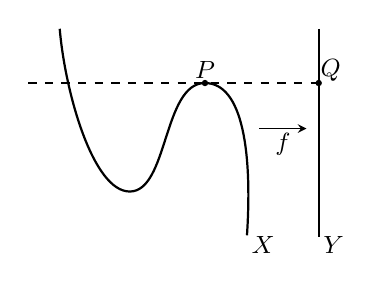
\begin{tikzpicture}[x=.63bp,y=-.63bp,every node/.style={font=\small,inner sep=1.5pt},>=stealth]
\draw[dashed,thin] (0,32) -- (166,32);
\draw[line width=.8pt] (18,1) .. controls (21,37) and (37,94) .. (58,94)
 .. controls (80,94) and (77,32) .. (101,32)
 .. controls (123,32) and (128,73) .. (125,119);
\draw[line width=.75pt] (166,1) -- (166,120);
\fill (101,32) circle[radius=1.15bp] node[above] {$P$};
\fill (166,32) circle[radius=1.15bp] node[above right=-1pt] {$Q$};
\draw[->] (132,58) -- node[below] {$f$} (159,58);
\node[below right] at (125,117) {$X$};
\node[below right] at (166,117) {$Y$};
\end{tikzpicture}\par\nobreak\smallskip
Figure 13.\enspace A finite morphism of curves.\par}

\smallskip
If $\operatorname{char}k=0$, or if $\operatorname{char}k=p$, and $p$ does not divide $e_P$, we say that the ramification is \emph{tame}. If $p$ does divide $e_P$, it is \emph{wild}.

Recall that we have defined a homomorphism $f^*\colon\operatorname{Div}Y\to\operatorname{Div}X$ of the groups of divisors, by setting
\[
f^*(Q)=\sum_{P\to Q}e_P\cdot P
\]
for any point $Q$ of $Y$, and extending by linearity (II, \Goto{sec-II-6}{\S6}). If $D$ is a divisor on $Y$, then $f^*(\mathcal L(D))\cong\mathcal L(f^*D)$ (II, Ex.~\Goto{ex-II-6.8}{6.8}), so that this $f^*$ on divisors is compatible with the homomorphism $f^*\colon\operatorname{Pic}Y\to\operatorname{Pic}X$ on invertible sheaves.
}
% Contents from body/page-314.tex.
\ChapterSheet{314}{300}{\Goto{p-307}{IV\quad Curves}}{%
\indent We say the morphism $f\colon X\to Y$ is \emph{separable} if $K(X)$ is a separable field extension of $K(Y)$.

\medskip
\noindent\hypertarget{result-IV-2.1}{}\textbf{Proposition 2.1.} \emph{Let $f\colon X\to Y$ be a finite separable morphism of curves. Then there is an exact sequence of sheaves on $X$,}
\[
0\to f^*\Omega_Y\to\Omega_X\to\Omega_{X/Y}\to0.
\]

\smallskip
\noindent\textsc{Proof.} From (II, \Goto{result-II-8.11}{8.11}) we have this exact sequence, but without the $0$ on the left. So we have only to show that $f^*\Omega_Y\to\Omega_X$ is injective. Since both are invertible sheaves on $X$, it will be sufficient to show that the map is nonzero at the generic point. But since $K(X)$ is separable over $K(Y)$, the sheaf $\Omega_{X/Y}$ is zero at the generic point of $X$, by (II, \Goto{result-II-8.6A}{8.6A}). Hence $f^*\Omega_Y\to\Omega_X$ is surjective at the generic point.

\medskip
Since $\Omega_Y$ and $\Omega_X$ correspond to the canonical divisors on $Y$ and $X$, respectively, we see that the sheaf of relative differentials $\Omega_{X/Y}$ measures their difference. So we will study this sheaf. For any point $P\in X$, let $Q=f(P)$, let $t$ be a local parameter at $Q$, and let $u$ be a local parameter at $P$. Then $dt$ is a generator of the free $\mathcal O_Q$-module $\Omega_{Y,Q}$, and $du$ is a generator of the free $\mathcal O_P$-module $\Omega_{X,P}$, by (II, \Goto{result-II-8.7}{8.7}) and (II, \Goto{result-II-8.8}{8.8}). In particular, there is a unique element $g\in\mathcal O_P$ such that $f^*dt=g\cdot du$. We denote this element by $dt/du$.

\medskip
\noindent\hypertarget{result-IV-2.2}{}\textbf{Proposition 2.2.} \emph{Let $f\colon X\to Y$ be a finite, separable morphism of curves. Then:}
\par{\itshape\leftskip=12pt
\hypertarget{result-IV-2.2a}{}(a) $\Omega_{X/Y}$ is a torsion sheaf on $X$, with support equal to the set of ramification points of $f$. In particular, $f$ is ramified at only finitely many points;

\hypertarget{result-IV-2.2b}{}(b) for each $P\in X$, the stalk $(\Omega_{X/Y})_P$ is a principal $\mathcal O_P$-module of finite length equal to $v_P(dt/du)$;

\hypertarget{result-IV-2.2c}{}(c) if $f$ is tamely ramified at $P$, then
\[
\operatorname{length}(\Omega_{X/Y})_P=e_P-1.
\]
If $f$ is wildly ramified, then the length is $> e_P-1$.\par}

\smallskip
\noindent\textsc{Proof.}\par
(a) The fact that $\Omega_{X/Y}$ is a torsion sheaf follows from \Goto{result-IV-2.1}{(2.1)} since $f^*\Omega_Y$ and $\Omega_X$ are both invertible sheaves on $X$. Now $(\Omega_{X/Y})_P=0$ if and only if $f^*dt$ is a generator for $\Omega_{X,P}$, using the above notation. But this happens if and only if $t$ is a local parameter for $\mathcal O_P$, i.e., $f$ is unramified at $P$.

(b) Indeed, from the exact sequence of \Goto{result-IV-2.1}{(2.1)}, we see that $(\Omega_{X/Y})_P\cong\Omega_{X,P}/f^*\Omega_{Y,Q}$, which is isomorphic as an $\mathcal O_P$-module to $\mathcal O_P/(dt/du)$.

(c) If $f$ has ramification index $e=e_P$, then we can write $t=au^e$ for some unit $a\in\mathcal O_P$. Then
\[
dt=aeu^{e-1}\,du+u^e\,da.
\]
}
% Contents from body/page-315.tex.
\ChapterSheet{315}{301}{\Goto{sec-IV-2}{2\quad Hurwitz's Theorem}}{%
If the ramification is tame, then $e$ is a nonzero element of $k$, so we have $v_P(dt/du)=e-1$. Otherwise $v_P(dt/du)\geq e$.

\medskip
\noindent\textbf{Definition.} Let $f\colon X\to Y$ be a finite, separable morphism of curves. Then we define the \emph{ramification divisor} of $f$ to be
\[
R=\sum_{P\in X}\operatorname{length}(\Omega_{X/Y})_P\cdot P.
\]

\medskip
\noindent\hypertarget{result-IV-2.3}{}\textbf{Proposition 2.3.} \emph{Let $f\colon X\to Y$ be a finite, separable morphism of curves. Let $K_X$ and $K_Y$ be the canonical divisors of $X$ and $Y$, respectively. Then}
\[
K_X\sim f^*K_Y+R.
\]

\smallskip
\noindent\textsc{Proof.} Considering the divisor $R$ as a closed subscheme of $X$, we see from \Goto{result-IV-2.2}{(2.2)} that its structure sheaf $\mathcal O_R$ is isomorphic to $\Omega_{X/Y}$. Tensoring the exact sequence of \Goto{result-IV-2.1}{(2.1)} with $\Omega_X^{-1}$, we can therefore write an exact sequence
\[
0\to f^*\Omega_Y\otimes\Omega_X^{-1}\to\mathcal O_X\to\mathcal O_R\to0.
\]
But by (II, \Goto{result-II-6.18}{6.18}), the ideal sheaf of $R$ is isomorphic to $\mathcal L(-R)$, so we have
\[
f^*\Omega_Y\otimes\Omega_X^{-1}\cong\mathcal L(-R).
\]
Now the result follows from taking associated divisors. (One can also prove this proposition by applying the operation $\det$ of (II, Ex.~\Goto{ex-II-6.11}{6.11}) to the exact sequence of \Goto{result-IV-2.1}{(2.1)}.)

\medskip
\noindent\hypertarget{result-IV-2.4}{}\textbf{Corollary 2.4} (Hurwitz). \emph{Let $f\colon X\to Y$ be a finite separable morphism of curves. Let $n=\deg f$. Then}
\[
2g(X)-2=n\cdot(2g(Y)-2)+\deg R.
\]
\emph{Furthermore, if $f$ has only tame ramification, then}
\[
\deg R=\sum_{P\in X}(e_P-1).
\]

\smallskip
\noindent\textsc{Proof.} We take the degrees of the divisors in \Goto{result-IV-2.3}{(2.3)}. The canonical divisor has degree $2g-2$ by \Goto{result-IV-1.3.3}{(1.3.3)}; $f^*$ multiplies degrees by $n$ (II, \Goto{result-II-6.9}{6.9}); and if the ramification is tame, $R$ has degree $\sum(e_P-1)$ by \Goto{result-IV-2.2}{(2.2)}.

\medskip
We complete our discussion of finite morphisms by describing what happens in the purely inseparable case. First we define the Frobenius morphism.

\medskip
\noindent\textbf{Definition.} Let $X$ be a scheme, all of whose local rings are of characteristic $p$ (i.e., contain $\mathbf Z/p$). We define the \emph{Frobenius morphism} $F\colon X\to X$ as follows: $F$ is the identity map on the topological space of $X$, and $F^\#\colon\mathcal O_X\to\mathcal O_X$ is the $p$th power map. Since the local rings are of characteristic $p$, $F^\#$ induces a local homomorphism on each local ring, so $F$ is indeed a morphism.
}
% Contents from body/page-316.tex.
\ChapterSheet{316}{302}{\Goto{p-307}{IV\quad Curves}}{%
\noindent\hypertarget{result-IV-2.4.1}{}\textbf{Remark 2.4.1.} If $\pi\colon X\to\operatorname{Spec}k$ is a scheme over a field $k$ of characteristic $p$, then
\EditionText{$F\colon X\to X$ is not $k$-linear. On the contrary, we have a commutative diagram}
\[
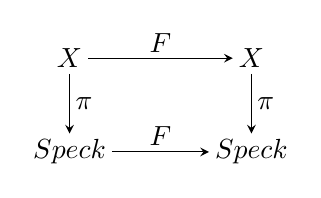
\begin{tikzpicture}[x=2.31cm,y=1.19cm,every node/.style={inner sep=2pt},>=stealth]
\node (a) at (0,0) {$X$};
\node (b) at (1,0) {$X$};
\node (c) at (0,-1) {$\operatorname{Spec}k$};
\node (d) at (1,-1) {$\operatorname{Spec}k$};
\draw[->] (a) -- node[above] {$F$} (b);
\draw[->] (a) -- node[right] {$\pi$} (c);
\draw[->] (b) -- node[right] {$\pi$} (d);
\draw[->] (c) -- node[above] {$F$} (d);
\end{tikzpicture}
\]
with the Frobenius morphism $F$ of $\operatorname{Spec}k$ (which corresponds to the $p$th power map of $k$ to itself).

We define a new scheme over $k$, $X_p$, to be the same scheme $X$, but with structural morphism $F\circ\pi$. Thus $k$ acts on $\mathcal O_{X_p}$ via $p$th powers. Then $F$ becomes a $k$-linear morphism $F'\colon X_p\to X$. We call this the \emph{$k$-linear Frobenius morphism}.

\medskip
\noindent\hypertarget{result-IV-2.4.2}{}\textbf{Example 2.4.2.} If $X$ is a scheme over $k$, then $X_p$ may or may not be isomorphic to $X$ as a scheme over $k$. For example, if $X=\operatorname{Spec}k[t]$, where $k$ is a perfect field, then $X_p$ is isomorphic to $X$, because the $p$th power map $k\to k$ is bijective. Under this identification, the $k$-linear Frobenius morphism $F'\colon X\to X$ corresponds to the homomorphism $k[t]\to k[t]$ defined by $t\mapsto t^p$. This is the morphism given in (I, Ex.~\Goto{ex-I-3.2}{3.2}).

\medskip
\noindent\hypertarget{result-IV-2.4.3}{}\textbf{Example 2.4.3.} If $X$ is a curve over $k$, an algebraically closed field of characteristic $p$, then $F'\colon X_p\to X$ is a finite morphism of degree $p$. It corresponds to the field inclusion $K\hookrightarrow K^{1/p}$, where $K$ is the function field of $X$, and $K^{1/p}$ is the field of $p$th roots of elements of $K$ in some fixed algebraic closure of $K$.

\medskip
\noindent\hypertarget{result-IV-2.5}{}\textbf{Proposition 2.5.} \emph{Let $f\colon X\to Y$ be a finite morphism of curves, and suppose that $K(X)$ is a purely inseparable field extension of $K(Y)$. Then $X$ and $Y$ are isomorphic as abstract schemes, and $f$ is a composition of $k$-linear Frobenius morphisms. In particular, $g(X)=g(Y)$.}

\smallskip
\noindent\textsc{Proof.} Let the degree of $f$ be $p^r$. Then $K(X)^{p^r}\subseteq K(Y)$, or in other words, $K(X)\subseteq K(Y)^{1/p^r}$. On the other hand, consider the $k$-linear Frobenius morphisms
\[
Y_{p^r}\xrightarrow{F'}Y_{p^{r-1}}\to\cdots\to Y_p\xrightarrow{F'}Y,
\]
where for each $i$, $Y_{p^i}=(Y_{p^{i-1}})_p$. The composition of these is a morphism $f'\colon Y_{p^r}\to Y$, also of degree $p^r$. Since $K(X)\subseteq K(Y)^{1/p^r}$, and both have the same degree over $K(Y)$, we conclude that $K(X)=K(Y)^{1/p^r}$. Since a curve is uniquely determined by its function field (I, \Goto{result-I-6.12}{6.12}), we have $X\cong Y_{p^r}$, and $f=f'$. Therefore $X$ and $Y$ are isomorphic as abstract schemes, and their genus (which does not depend on the $k$-structure) is the same.
}
% Contents from body/page-317.tex.
\ChapterSheet{317}{303}{\Goto{sec-IV-2}{2\quad Hurwitz's Theorem}}{%
\noindent\hypertarget{result-IV-2.5.1}{}\textbf{Example 2.5.1.} If $X=Y_p$, and $f\colon X\to Y$ is the $k$-linear Frobenius morphism, then $f$ is ramified everywhere, with ramification index $p$. Indeed, $f$ is the identity on point sets, but $p$th power on structure sheaves. So if $t\in\mathcal O_P$ is a local parameter, $f^\#t=t^p$. Since $d(t^p)=0$, the map $f^*\Omega_Y\to\Omega_X$ is the zero map, so $\Omega_{X/Y}\cong\Omega_X$.

\medskip
\noindent\hypertarget{result-IV-2.5.2}{}\textbf{Example 2.5.2.} If $f\colon X\to Y$ is separable, then the degree of the ramification divisor $R$ is always an even number. This follows from the formula of \Goto{result-IV-2.4}{(2.4)}.

\medskip
\noindent\hypertarget{result-IV-2.5.3}{}\textbf{Example 2.5.3.} An \emph{\'etale covering} of a scheme $Y$ is a scheme $X$, together with a finite \'etale morphism $f\colon X\to Y$. It is called \emph{trivial} \EditionText{if $X$ is isomorphic to a finite disjoint union of copies of $Y$.} $Y$ is called \emph{simply connected} if it has no nontrivial \'etale coverings.

Now we show that $\Proj^1$ is simply connected. Indeed, let $f\colon X\to\Proj^1$ be an \'etale covering. We may assume $X$ is connected. Then $X$ is smooth over $k$ since $f$ is \'etale (III, \Goto{result-III-10.1}{10.1}), and $X$ is proper over $k$ since $f$ is finite, so $X$ is a curve (note connected and regular imply irreducible). Again since $f$ is \'etale, $f$ is separable, so we can apply Hurwitz's theorem. Since $f$ is unramified, $R=0$ so we have
\[
2g(X)-2=n(-2).
\]
Since $g(X)\geq0$, the only way this can happen is for $g(X)=0$ and $n=1$. Thus $X=\Proj^1$.

\medskip
\noindent\hypertarget{result-IV-2.5.4}{}\textbf{Example 2.5.4.} If $f\colon X\to Y$ is any finite morphism of curves, then $g(X)\geq g(Y)$. We can factor the field extension $K(Y)\subseteq K(X)$ into a separable extension followed by a purely inseparable extension. Since the genus doesn't change for a purely inseparable extension \Goto{result-IV-2.5}{(2.5)}, we reduce to the case $f$ separable. If $g(Y)=0$, there is nothing to prove, so we may assume $g(Y)\geq1$. Then we rewrite the formula of \Goto{result-IV-2.4}{(2.4)} as
\[
g(X)=g(Y)+(n-1)(g(Y)-1)+\tfrac12\deg R.
\]
Since $n-1\geq0$, $g(Y)-1\geq0$, and $\deg R\geq0$, we are done. By the way, this shows also that equality occurs (for $f$ separable\EditionText{}) only if $n=1$, or $g(Y)=1$ and $f$ is unramified.

\medskip
\noindent\hypertarget{result-IV-2.5.5}{}\textbf{Example 2.5.5} (L\"uroth's Theorem). This says that if $L$ is a subfield of a pure transcendental extension $k(t)$ of $k$, containing $k$, then $L$ is also pure transcendental. We may assume that $L\ne k$, so that $L$ has transcendence degree $1$ over $k$. Then $L$ is a function field of a curve $Y$, and the inclusion $L\subseteq k(t)$ corresponds to a finite morphism $f\colon\Proj^1\to Y$. By \Goto{result-IV-2.5.4}{(2.5.4)} we conclude that $g(Y)=0$, so by \Goto{result-IV-1.3.5}{(1.3.5)}, $Y\cong\Proj^1$. Hence $L\cong k(u)$ for some $u$.
}
% Contents from body/page-318.tex.
\ChapterSheet[11.3]{318}{304}{\Goto{p-307}{IV\quad Curves}}{%
\indent\emph{Note:} This proof is only for $k$ algebraically closed, but the theorem is true for any field $k$.
\EditionText{An analogous result over $k$ algebraically closed is true also in dimension $2$ (V, \Goto{result-V-6.2.1}{6.2.1}).}
In dimension $3$ the corresponding statement is false, because of the existence of nonrational unirational $3$-folds---see Clemens and Griffiths \Goto{bib-clemens-griffiths-1}{[1]} and Iskovskih and Manin \Goto{bib-iskovskih-manin-1}{[1]}.

\medskip
\noindent\textsc{Exercises}\par\nobreak\smallskip
{\fontsize{9.1}{10.17}\selectfont\setlength{\parskip}{.45pt}\leftskip=20pt\relax
\noindent\hypertarget{ex-IV-2.1}{}\llap{\textbf{2.1.}\enspace}Use \Goto{result-IV-2.5.3}{(2.5.3)} to show that $\Proj^n$ is simply connected.

\smallskip
\noindent\hypertarget{ex-IV-2.2}{}\llap{\textbf{2.2.}\enspace}\emph{Classification of Curves of Genus $2$.} Fix an algebraically closed field $k$ of characteristic $\ne2$.
{\advance\leftskip by 13pt\par
\noindent\hypertarget{ex-IV-2.2a}{}\llap{(a)\enspace}If $X$ is a curve of genus $2$ over $k$, the canonical linear system $|K|$ determines a finite morphism $f\colon X\to\Proj^1$ of degree $2$ (Ex.~\Goto{ex-IV-1.7}{1.7}). Show that it is ramified at exactly $6$ points, with ramification index $2$ at each one. Note that $f$ is uniquely determined, up to an automorphism of $\Proj^1$, so $X$ determines an (unordered) set of $6$ points of $\Proj^1$, up to an automorphism of $\Proj^1$.

\noindent\hypertarget{ex-IV-2.2b}{}\llap{(b)\enspace}Conversely, given six distinct elements $\alpha_1,\ldots,\alpha_6\in k$, let $K$ be the extension of $k(x)$ determined by the equation $z^2=(x-\alpha_1)\cdots(x-\alpha_6)$. Let $f\colon X\to\Proj^1$ be the corresponding morphism of curves. Show that $g(X)=2$, the map $f$ is the same as the one determined by the canonical linear system, and $f$ is ramified over the six points $x=\alpha_i$ of $\Proj^1$, and nowhere else. (Cf. (II, Ex.~\Goto{ex-II-6.4}{6.4}).)

\noindent\hypertarget{ex-IV-2.2c}{}\llap{(c)\enspace}Using (I, Ex.~\Goto{ex-I-6.6}{6.6}), show that if $P_1,P_2,P_3$ are three distinct points of $\Proj^1$, then there exists a unique $\varphi\in\operatorname{Aut}\Proj^1$ such that $\varphi(P_1)=0$, $\varphi(P_2)=1$, $\varphi(P_3)=\infty$. Thus in \Goto{ex-IV-2.2a}{(a)}, if we order the six points of $\Proj^1$, and then normalize by sending the first three to $0,1,\infty$, respectively, we may assume that $X$ is ramified over $0,1,\infty,\beta_1,\beta_2,\beta_3$, where $\beta_1,\beta_2,\beta_3$ are three distinct elements of $k$, $\ne0,1$.

\noindent\hypertarget{ex-IV-2.2d}{}\llap{(d)\enspace}Let $\Sigma_6$ be the symmetric group on $6$ letters. Define an action of $\Sigma_6$ on
\EditionText{sets of three distinct elements $\beta_1,\beta_2,\beta_3$ of $k$, $\ne0,1$, as follows: reorder the set $0,1,\infty,\beta_1,\beta_2,\beta_3$ according to a given element $\sigma\in\Sigma_6$,}
then renormalize as in \Goto{ex-IV-2.2c}{(c)} so that the first three become $0,1,\infty$ again. Then the last three are the new $\beta'_1,\beta'_2,\beta'_3$.

\noindent\hypertarget{ex-IV-2.2e}{}\llap{(e)\enspace}Summing up, conclude that there is a one-to-one correspondence between the set of isomorphism classes of curves of genus $2$ over $k$, and \EditionText{triples} of distinct elements $\beta_1,\beta_2,\beta_3$ of $k$, $\ne0,1$, modulo the action of $\Sigma_6$ described in \Goto{ex-IV-2.2d}{(d)}. In particular, there are many non-isomorphic curves of genus $2$. We say that curves of genus $2$ depend on three parameters, since they correspond to the points of an open subset of $\AffSpace[k]{3}$ modulo a finite group.\par}

\smallskip
\noindent\hypertarget{ex-IV-2.3}{}\llap{\textbf{2.3.}\enspace}\emph{Plane Curves.} Let $X$ be a curve of degree $d$\EditionText{} in $\Proj^2$. For each point $P\in X$, let $T_P(X)$ be the tangent line to $X$ at $P$ (I, Ex.~\Goto{ex-I-7.3}{7.3}). Considering $T_P(X)$ as a point of the dual projective plane $(\Proj^2)^*$, the map $P\mapsto T_P(X)$ gives a morphism of $X$ to its \emph{dual curve} $X^*$ in $(\Proj^2)^*$ (I, Ex.~\Goto{ex-I-7.3}{7.3}). Note that even though $X$ is nonsingular, $X^*$ in general will have singularities. We assume $\operatorname{char}k=0$ below.
{\advance\leftskip by 13pt\par
\noindent\hypertarget{ex-IV-2.3a}{}\llap{(a)\enspace}Fix a line $L\subseteq\Proj^2$ which is not tangent to $X$. Define a morphism $\varphi\colon X\to L$ by $\varphi(P)=T_P(X)\cap L$, for each point $P\in X$. Show that $\varphi$ is ramified at $P$ if and only if either (1) $P\in L$, or (2) $P$ is an \emph{inflection point} of $X$, which means that the intersection multiplicity (I, Ex.~\Goto{ex-I-5.4}{5.4}) of $T_P(X)$ with $X$ at $P$ is $\geq3$. Conclude that $X$ has only finitely many inflection points.\par}\par}
}
% Contents from body/page-319.tex.
\ChapterSheet{319}{305}{\Goto{sec-IV-2}{2\quad Hurwitz's Theorem}}{%
{\fontsize{9.1}{10.09}\selectfont\setlength{\parskip}{.45pt}\leftskip=19pt\relax
{\advance\leftskip by 12pt
\noindent\hypertarget{ex-IV-2.3b}{}\llap{(b)\enspace}A line of $\Proj^2$ is a \emph{multiple tangent} of $X$ if it is tangent to $X$ at more than one point. It is a \emph{bitangent} if it is tangent to $X$ at exactly two points. If $L$ is a multiple tangent of $X$, tangent to $X$ at the points $P_1,\ldots,P_r$, and if none of the $P_i$ is an inflection point, show that the corresponding point of the dual curve $X^*$ is an \emph{ordinary $r$-fold point}, which means a point of multiplicity $r$ with distinct tangent directions (I, Ex.~\Goto{ex-I-5.3}{5.3}). Conclude that $X$ has only finitely many multiple tangents.

\noindent\hypertarget{ex-IV-2.3c}{}\llap{(c)\enspace}Let $O\in\Proj^2$ be a point which is not on $X$, nor on any inflectional or multiple tangent of $X$. Let $L$ be a line not containing $O$. Let $\psi\colon X\to L$ be the morphism defined by projection from $O$. Show that $\psi$ is ramified at a point $P\in X$ if and only if the line $OP$ is tangent to $X$ at $P$, and in that case the ramification index is $2$. Use Hurwitz's theorem and (I, Ex.~\Goto{ex-I-7.2}{7.2}) to conclude that there are exactly $d(d-1)$ tangents of $X$ passing through $O$. Hence the degree of the dual curve (sometimes called the \emph{class} of $X$) is $d(d-1)$.

\noindent\hypertarget{ex-IV-2.3d}{}\llap{(d)\enspace}Show that for all but a finite number of points of $X$, a point $O$ of $X$ lies on exactly $(d+1)(d-2)$ tangents of $X$, not counting the tangent at $O$.

\noindent\hypertarget{ex-IV-2.3e}{}\llap{(e)\enspace}Show that the degree of the morphism $\varphi$ of \Goto{ex-IV-2.3a}{(a)} is $d(d-1)$. Conclude that if $d\geq2$, then $X$ has $3d(d-2)$ inflection points, properly counted. (If $T_P(X)$ has intersection multiplicity $r$ with $X$ at $P$, then $P$ should be counted $r-2$ times as an inflection point. If $r=3$ we call it an \emph{ordinary inflection point}.) Show that an ordinary inflection point of $X$ corresponds to an ordinary cusp of the dual curve $X^*$.

\noindent\hypertarget{ex-IV-2.3f}{}\llap{(f)\enspace}Now let $X$ be a plane curve of degree $d\geq2$, and assume that the dual curve $X^*$ has only nodes and ordinary cusps as singularities (which should be true for sufficiently general $X$). Then show that $X$ has exactly $\tfrac12d(d-2)(d-3)(d+3)$ bitangents. [\emph{Hint:} Show that $X$ is the normalization of $X^*$. Then calculate $p_a(X^*)$ two ways: once as a plane curve of degree $d(d-1)$, and once using (Ex.~\Goto{ex-IV-1.8}{1.8}).]

\noindent\hypertarget{ex-IV-2.3g}{}\llap{(g)\enspace}For example, a plane cubic curve has exactly $9$ inflection points, all ordinary. The line joining any two of them intersects the curve in a third one.

\noindent\hypertarget{ex-IV-2.3h}{}\llap{(h)\enspace}\EditionText{A plane quartic curve has exactly $28$ bitangents. (This holds even if the curve has a tangent with four-fold contact, in which case the dual curve $X^*$ has a tacnode.)}\par}

\smallskip
\noindent\hypertarget{ex-IV-2.4}{}\llap{\textbf{2.4.}\enspace}\emph{A Funny Curve in Characteristic $p$.} Let $X$ be the plane quartic curve $x^3y+y^3z+z^3x=0$ over a field of characteristic $3$. Show that $X$ is nonsingular, every point of $X$ is an inflection point, the dual curve $X^*$ is isomorphic to $X$, but the natural map $X\to X^*$ is purely inseparable.

\smallskip
\noindent\hypertarget{ex-IV-2.5}{}\llap{\textbf{2.5.}\enspace}\emph{Automorphisms of a Curve of Genus $\geq2$.} Prove the theorem of Hurwitz \Goto{bib-hurwitz-1}{[1]} that a curve $X$ of genus $g\geq2$ over a field of characteristic $0$ has at most $84(g-1)$ automorphisms. We will see later (Ex.~\Goto{ex-IV-5.2}{5.2}) or (V, Ex.~\Goto{ex-V-1.11}{1.11}) that the group $G=\operatorname{Aut}X$ is finite. So let $G$ have order $n$. Then $G$ acts on the function field $K(X)$. Let $L$ be the fixed field. Then the field extension $L\subseteq K(X)$ corresponds to a finite morphism of curves $f\colon X\to Y$ of degree $n$.
{\advance\leftskip by 12pt\par
\noindent\hypertarget{ex-IV-2.5a}{}\llap{(a)\enspace}If $P\in X$ is a ramification point, and $e_P=r$, show that $f^{-1}f(P)$ consists of exactly $n/r$ points, each having ramification index $r$. Let $P_1,\ldots,P_s$ be a maximal set of ramification points of $X$ lying over distinct points of $Y$, and let $e_{P_i}=r_i$. Then show that Hurwitz's theorem implies that
\[
(2g-2)/n=2g(Y)-2+\sum_{i=1}^s(1-1/r_i).
\]\par}\par}
}
% Contents from body/page-320.tex.
\ChapterSheet{320}{306}{\Goto{p-307}{IV\quad Curves}}{%
{\fontsize{9.2}{10.25}\selectfont\setlength{\parskip}{.55pt}\leftskip=21pt\relax
{\advance\leftskip by 13pt
\noindent\hypertarget{ex-IV-2.5b}{}\llap{(b)\enspace}Since $g\geq2$, the left hand side of the equation is $>0$. Show that if $g(Y)\geq0$, $s\geq0$, $r_i\geq2$, $i=1,\ldots,s$ are integers such that
\[
2g(Y)-2+\sum_{i=1}^s(1-1/r_i)>0,
\]
then the minimum value of this expression is $1/42$. Conclude that $n\leq84(g-1)$. See (Ex.~\Goto{ex-IV-5.7}{5.7}) for an example where this maximum is achieved.\par}

\emph{Note:} It is known that this maximum is achieved for infinitely many values of $g$ (Macbeath \Goto{bib-macbeath-1}{[1]}). Over a field of characteristic $p>0$, the same bound holds, provided $p>g+1$, with one exception, namely the hyperelliptic curve $y^2=x^p-x$, which has $p=2g+1$ and $2p(p^2-1)$ automorphisms (Roquette \Goto{bib-roquette-1}{[1]}). For other bounds on the order of the group of automorphisms in characteristic $p$, see Singh \Goto{bib-singh-1}{[1]} and Stichtenoth \Goto{bib-stichtenoth-1}{[1]}.

\smallskip
\noindent\hypertarget{ex-IV-2.6}{}\llap{\textbf{2.6.}\enspace}\emph{$f_*$ for Divisors.} Let $f\colon X\to Y$ be a finite morphism of curves of degree $n$. We define a homomorphism $f_*\colon\operatorname{Div}X\to\operatorname{Div}Y$ by $f_*(\sum n_iP_i)=\sum n_if(P_i)$ for any divisor $D=\sum n_iP_i$ on $X$.
{\advance\leftskip by 13pt\par
\noindent\hypertarget{ex-IV-2.6a}{}\llap{(a)\enspace}For any locally free sheaf $\mathcal E$ on $Y$, of rank $r$, we define $\det\mathcal E=\bigwedge^r\mathcal E\in\operatorname{Pic}Y$ (II, Ex.~\Goto{ex-II-6.11}{6.11}). In particular, for any invertible sheaf $\mathcal M$ on $X$, $f_*\mathcal M$ is locally free of rank $n$ on $Y$, so we can consider $\det f_*\mathcal M\in\operatorname{Pic}Y$. Show that for any divisor $D$ on $X$,
\[
\det(f_*\mathcal L(D))\cong(\det f_*\mathcal O_X)\otimes\mathcal L(f_*D).
\]
Note in particular that $\det(f_*\mathcal L(D))\ne\mathcal L(f_*D)$ in general! [\emph{Hint:} First consider an effective divisor $D$, apply $f_*$ to the exact sequence $0\to\mathcal L(-D)\to\mathcal O_X\to\mathcal O_D\to0$, and use (II, Ex.~\Goto{ex-II-6.11}{6.11}).]

\noindent\hypertarget{ex-IV-2.6b}{}\llap{(b)\enspace}Conclude that $f_*D$ depends only on the linear equivalence class of $D$, so there is an induced homomorphism $f_*\colon\operatorname{Pic}X\to\operatorname{Pic}Y$. Show that $f_*\circ f^*\colon\operatorname{Pic}Y\to\operatorname{Pic}Y$ is just multiplication by $n$.

\noindent\hypertarget{ex-IV-2.6c}{}\llap{(c)\enspace}Use duality for a finite flat morphism (III, Ex.~\Goto{ex-III-6.10}{6.10}) and (III, Ex.~\Goto{ex-III-7.2}{7.2}) to show that
\[
\det f_*\Omega_X\cong(\det f_*\mathcal O_X)^{-1}\otimes\Omega_Y^{\otimes n}.
\]

\noindent\hypertarget{ex-IV-2.6d}{}\llap{(d)\enspace}Now assume that $f$ is separable, so we have the ramification divisor $R$. We define the \emph{branch divisor} $B$ to be the divisor $f_*R$ on $Y$. Show that
\[
(\det f_*\mathcal O_X)^2\cong\mathcal L(-B).
\]\par}

\smallskip
\noindent\hypertarget{ex-IV-2.7}{}\llap{\textbf{2.7.}\enspace}\emph{\'Etale Covers of Degree $2$.} Let $Y$ be a curve over a field $k$ of characteristic $\ne2$. We show there is a one-to-one correspondence between
\EditionText{finite \'etale morphisms $f\colon X\to Y$ of degree $2$,}
and $2$-torsion elements of $\operatorname{Pic}Y$, i.e., invertible sheaves $\mathcal L$ on $Y$ with $\mathcal L^2\cong\mathcal O_Y$.
{\advance\leftskip by 13pt\par
\noindent\hypertarget{ex-IV-2.7a}{}\llap{(a)\enspace}Given an \'etale morphism $f\colon X\to Y$ of degree $2$, there is a natural map $\mathcal O_Y\to f_*\mathcal O_X$. Let $\mathcal L$ be the cokernel. Then $\mathcal L$ is an invertible sheaf on $Y$, $\mathcal L\cong\det f_*\mathcal O_X$, and so $\mathcal L^2\cong\mathcal O_Y$ by (Ex.~\Goto{ex-IV-2.6}{2.6})\EditionText{}. Thus an \'etale cover of degree $2$ determines a $2$-torsion element in $\operatorname{Pic}Y$.

\noindent\hypertarget{ex-IV-2.7b}{}\llap{(b)\enspace}Conversely, given a $2$-torsion element $\mathcal L$ in $\operatorname{Pic}Y$, define an $\mathcal O_Y$-algebra structure on $\mathcal O_Y\oplus\mathcal L$ by $\langle a,b\rangle\cdot\langle a',b'\rangle=\langle aa'+\varphi(b\otimes b'),ab'+a'b\rangle$, where $\varphi$ is an isomorphism of $\mathcal L\otimes\mathcal L\to\mathcal O_Y$. Then take $X=\operatorname{\mathbf{Spec}}(\mathcal O_Y\oplus\mathcal L)$ (II, Ex.~\Goto{ex-II-5.17}{5.17}). Show that $X$ is an \'etale cover of $Y$.

\noindent\hypertarget{ex-IV-2.7c}{}\llap{(c)\enspace}Show that these two processes are inverse to each other. [\emph{Hint:} Let $\tau\colon X\to X$ be the involution which interchanges the points of each fibre of $f$. Use the\par}\par}
}
% Contents from body/page-321.tex.
\BookMark{1}{4.3  Embeddings in Projective Space}{sec-IV-3}
\ChapterSheet{321}{307}{3\quad Embeddings in Projective Space}{%
{\fontsize{9.2}{10.55}\selectfont\leftskip=21pt\relax
{\advance\leftskip by 13pt
\noindent\emph{trace map} $a\mapsto a+\tau(a)$ from $f_*\mathcal O_X\to\mathcal O_Y$ to show that the sequence of $\mathcal O_Y$-modules in \Goto{ex-IV-2.7a}{(a)}
\[
0\to\mathcal O_Y\to f_*\mathcal O_X\to\mathcal L\to0
\]
is split exact.\par}

\emph{Note.} This is a special case of the more general fact that for $(n,\operatorname{char}k)=1$, the
\EditionText{\'etale Galois covers of $Y$ with group $\mathbf Z/n\mathbf Z$ are classified by the \'etale cohomology group $H^1_{\mathrm{\acute{e}t}}(Y,\mathbf Z/n\mathbf Z)$, which is equal to the group of $n$-torsion points of $\operatorname{Pic}Y$.}
See Serre \Goto{bib-serre-6}{[6]}.\par}

\vspace{20pt}
\noindent\hypertarget{sec-IV-3}{}{\large\bfseries 3\quad Embeddings in Projective Space}\par\nobreak\vspace{9pt}
\noindent In this section we study embeddings of a curve in projective space. We will show that any curve can be embedded in $\Proj^3$. Furthermore, any curve can be mapped birationally into $\Proj^2$ in such a way that the image has at most nodes as singularities.

Recall that an invertible sheaf $\mathcal L$ on a curve $X$ is \emph{very ample} (II, \Goto{sec-II-5}{\S5}) if it is isomorphic to $\mathcal O_X(1)$ for some immersion of $X$ in a projective space. It is \emph{ample} (II, \Goto{sec-II-7}{\S7}) if for any coherent sheaf $\mathcal F$ on $X$, the sheaf $\mathcal F\otimes\mathcal L^n$ is generated by global sections for $n\gg0$. We have seen that $\mathcal L$ is ample if and only if $\mathcal L^n$ is very ample for some $n>0$ (II, \Goto{result-II-7.6}{7.6}). If $D$ is a divisor on $X$, we will say $D$ is \emph{ample} or \emph{very ample} if $\mathcal L(D)$ is.

Recall that a \emph{linear system} is a set $\mathfrak d$ of effective divisors, which forms a linear subspace of a complete linear system $|D|$. A point $P$ is a \emph{base point} of the linear system $\mathfrak d$ if $P\in\operatorname{Supp}D$ for all $D\in\mathfrak d$. We have seen that a complete linear system $|D|$ is base-point free if and only if $\mathcal L(D)$ is generated by global sections (II, \Goto{result-II-7.8}{7.8}).

Our first result is a reinterpretation in the case of curves of the criterion of (II, \Goto{sec-II-7}{\S7}) for when a linear system gives rise to a closed immersion into projective space.

\medskip
\noindent\hypertarget{result-IV-3.1}{}\textbf{Proposition 3.1.} \emph{Let $D$ be a divisor on a curve $X$. Then:}
\par{\itshape\leftskip=12pt
\hypertarget{result-IV-3.1a}{}(a) the complete linear system $|D|$ has no base points if and only if for every point $P\in X$,
\[
\dim|D-P|=\dim|D|-1;
\]

\hypertarget{result-IV-3.1b}{}(b) $D$ is very ample if and only if for every two points $P,Q\in X$ (including the case $P=Q$),
\[
\dim|D-P-Q|=\dim|D|-2.
\]\par}

\smallskip
\noindent\textsc{Proof.} First we consider the exact sequence of sheaves
\[
0\to\mathcal L(D-P)\to\mathcal L(D)\to k(P)\to0.
\]
Taking global sections, we have
\[
0\to\Gamma(X,\mathcal L(D-P))\to\Gamma(X,\mathcal L(D))\to k,
\]
}
% Contents from body/page-322.tex.
\ChapterSheet{322}{308}{\Goto{p-307}{IV\quad Curves}}{%
so in any case, we see that $\dim|D-P|$ is equal to either $\dim|D|$ or $\dim|D|-1$. Furthermore, sending a divisor $E$ to $E+P$ defines a linear map
\[
\varphi\colon |D-P|\to|D|
\]
which is clearly injective. Therefore, the dimensions of these two linear systems are equal if and only if $\varphi$ is surjective. On the other hand, $\varphi$ is surjective if and only if $P$ is a base point of $|D|$, so this proves \Goto{result-IV-3.1a}{(a)}.

To prove \Goto{result-IV-3.1b}{(b)}, we may assume that $|D|$ has no base points. Indeed, this is true if $D$ is very ample. On the other hand, if $D$ satisfies the condition of \Goto{result-IV-3.1b}{(b)}, then we must a fortiori have
\[
\dim|D-P|=\dim|D|-1
\]
for every $P\in X$, so $|D|$ has no base points.

This being the case, $|D|$ determines a morphism of $X$ to $\Proj^n$ (II, \Goto{result-II-7.1}{7.1}) and (II, \Goto{result-II-7.8.1}{7.8.1}), so the question is whether that morphism is a closed immersion. We use the criterion of (II, \Goto{result-II-7.3}{7.3}) and (II, \Goto{result-II-7.8.2}{7.8.2}), so we have to see whether $|D|$ separates points and separates tangent vectors. The first condition says that for any two distinct points $P,Q\in X$, $Q$ is not a base point of $|D-P|$. By \Goto{result-IV-3.1a}{(a)} this is equivalent to saying
\[
\dim|D-P-Q|=\dim|D|-2.
\]
The second condition says that for any point $P\in X$, there is a divisor $D'\in|D|$ such that $P$ occurs with multiplicity $1$ in $D'$, because $\dim T_P(X)=1$, and $\dim T_P(D')=0$ if $P$ has multiplicity $1$ in $D'$, $1$ if $P$ has higher multiplicity. But this just says $P$ is not a base point of $|D-P|$, or, using \Goto{result-IV-3.1a}{(a)} again,
\[
\dim|D-2P|=\dim|D|-2.
\]
Thus our result follows from (II, \Goto{result-II-7.3}{7.3}).

\medskip
\noindent\hypertarget{result-IV-3.2}{}\textbf{Corollary 3.2.} \emph{Let $D$ be a divisor on a curve $X$ of genus $g$.}
\par{\itshape\leftskip=12pt
\hypertarget{result-IV-3.2a}{}(a) If $\deg D\geq2g$, then $|D|$ has no base points.

\hypertarget{result-IV-3.2b}{}(b) If $\deg D\geq2g+1$, then $D$ is very ample.\par}

\smallskip
\noindent\textsc{Proof.} In case \Goto{result-IV-3.2a}{(a)}, both $D$ and $D-P$ are nonspecial \Goto{result-IV-1.3.4}{(1.3.4)}, so by Riemann--Roch, $\dim|D-P|=\dim|D|-1$. In case \Goto{result-IV-3.2b}{(b)}, $D$ and $D-P-Q$ are both nonspecial, so $\dim|D-P-Q|=\dim|D|-2$ again by Riemann--Roch.

\medskip
\noindent\hypertarget{result-IV-3.3}{}\textbf{Corollary 3.3.} \emph{A divisor $D$ on a curve $X$ is ample if and only if $\deg D>0$.}

\smallskip
\noindent\textsc{Proof.} If $D$ is ample, some multiple is very ample (II, \Goto{result-II-7.6}{7.6}), so $nD\sim H$ where $H$ is a hyperplane section for a projective embedding, so $\deg H>0$, hence $\deg D>0$. Conversely, if $\deg D>0$, then for $n\gg0$, $\deg nD\geq2g(X)+1$, so by \Goto{result-IV-3.2}{(3.2)}, $nD$ is very ample, and so $D$ is ample (II, \Goto{result-II-7.6}{7.6}).

\medskip
\noindent\hypertarget{result-IV-3.3.1}{}\textbf{Example 3.3.1.} If $g=0$, then $D$ is ample $\Leftrightarrow$ very ample $\Leftrightarrow\deg D>0$. Since $X\cong\Proj^1$ \Goto{result-IV-1.3.5}{(1.3.5)}, this is just (II, \Goto{result-II-7.6.1}{7.6.1}).
}
% Contents from body/page-323.tex.
\ChapterSheet{323}{309}{\Goto{sec-IV-3}{3\quad Embeddings in Projective Space}}{%
\noindent\hypertarget{result-IV-3.3.2}{}\textbf{Example 3.3.2.} Let $X$ be a curve, and let $D$ be a very ample divisor on $X$, corresponding to a closed immersion $\varphi\colon X\to\Proj^n$. Then the degree of $\varphi(X)$, as defined in (I, \Goto{sec-I-7}{\S7}) for a projective variety, is just equal to $\deg D$ (II, Ex.~\Goto{ex-II-6.2}{6.2}).

\medskip
\noindent\hypertarget{result-IV-3.3.3}{}\textbf{Example 3.3.3.} Let $X$ be an elliptic curve, i.e., $g=1$ \Goto{result-IV-1.3.6}{(1.3.6)}. Then any divisor $D$ of degree $3$ is very ample. Such a divisor is nonspecial, so by Riemann--Roch, $\dim|D|=2$. Thus we see that any elliptic curve can be embedded in $\Proj^2$ as a cubic curve. (Conversely, of course, any nonsingular plane cubic is elliptic, by the genus formula (I, Ex.~\Goto{ex-I-7.2}{7.2}).)

In the case $g=1$ we can actually say $D$ very ample $\Leftrightarrow\deg D\geq3$. Because if $\deg D=2$, then by Riemann--Roch, $\dim|D|=1$, so $|D|$ defines a morphism of $X$ to $\Proj^1$, which cannot be a closed immersion.

\medskip
\noindent\hypertarget{result-IV-3.3.4}{}\textbf{Example 3.3.4.} If $g=2$, then any divisor $D$ of degree $5$ is very ample. By Riemann--Roch, $\dim|D|=3$, so any curve of genus $2$ can be embedded in $\Proj^3$ as a curve of degree $5$.

\medskip
\noindent\hypertarget{result-IV-3.3.5}{}\textbf{Example 3.3.5.} The result of \Goto{result-IV-3.2}{(3.2)} is not the best possible in general. For example, if $X$ is a plane curve of degree $4$, then $D=X.H$ is a very ample divisor of degree $4$, but $g=3$ so $2g+1=7$.

\medskip
Our next objective is to show that any curve can be embedded in $\Proj^3$. For this purpose we consider a curve $X\subseteq\Proj^n$, take a point $O\notin X$, and project $X$ from $O$ into $\Proj^{n-1}$ (I, Ex.~\Goto{ex-I-3.14}{3.14}). This gives a morphism of $X$ into $\Proj^{n-1}$, and we investigate when it is a closed immersion.

If $P,Q$ are two distinct points of $X$, we define the \emph{secant line} determined by $P$ and $Q$ to be the line in $\Proj^n$ joining $P$ and $Q$. If $P$ is a point of $X$, we define the \emph{tangent line} to $X$ at $P$ to be the unique line $L\subseteq\Proj^n$ passing through $P$, whose tangent space $T_P(L)$ is equal to $T_P(X)$ as a subspace of $T_P(\Proj^n)$.

\medskip
\noindent\hypertarget{result-IV-3.4}{}\textbf{Proposition 3.4.} \emph{Let $X$ be a curve in $\Proj^n$, let $O$ be a point not on $X$, and let $\varphi\colon X\to\Proj^{n-1}$ be the morphism determined by projection from $O$. Then $\varphi$ is a closed immersion if and only if}
\par{\itshape\leftskip=11pt
\noindent\hypertarget{result-IV-3.4-1}{}(1) $O$ is not on any secant line of $X$, and

\noindent\hypertarget{result-IV-3.4-2}{}(2) $O$ is not on any tangent line of $X$.\par}

\smallskip
\noindent\textsc{Proof.} The morphism $\varphi$ corresponds (II, \Goto{result-II-7.8.1}{7.8.1}) to the linear system cut out on $X$ by the hyperplanes $H$ of $\Proj^n$ passing through $O$. So $\varphi$ is a closed immersion if and only if this linear system separates points and separates tangent vectors on $X$ (II, \Goto{result-II-7.8.2}{7.8.2}). If $P,Q$ are two distinct points on $X$, then $\varphi$ separates them if and only if there is an $H$ containing $O$ and $P$, but not $Q$. This is possible if and only if $O$ is not on the line $PQ$. If $P\in X$, then $\varphi$ separates tangent vectors at $P$ if and only if there is an $H$ containing $O$ and $P$, and meeting $X$ at $P$ with multiplicity $1$. This is possible if and only if $O$ is not on the tangent line at $P$.
}
% Contents from body/page-324.tex.
\ChapterSheet{324}{310}{\Goto{p-307}{IV\quad Curves}}{%
\noindent\hypertarget{result-IV-3.5}{}\textbf{Proposition 3.5.} \emph{If $X$ is a curve in $\Proj^n$, with $n\geq4$, then there is a point $O\notin X$ such that the projection from $O$ gives a closed immersion of $X$ into $\Proj^{n-1}$.}

\smallskip
\noindent\textsc{Proof.} Let $\operatorname{Sec}X$ be the union of all secant lines of $X$. We call this the \emph{secant variety} of $X$.
\EditionText{It is a locally closed subset of $\Proj^n$, of dimension $\leq3$, since (at least locally) it is the image of a morphism from $(X\times X-\Delta)\times\Proj^1$ to $\Proj^n$ which sends $\langle P,Q,t\rangle$ to the point $t$ on the secant line through $P$ and $Q$, suitably parametrized.}

Let $\operatorname{Tan}X$, the \emph{tangent variety} of $X$, be the union of all tangent lines of $X$. It is a closed subset of $\Proj^n$, of dimension $\leq2$, because it is locally an image of $X\times\Proj^1$.

Since $n\geq4$, $\operatorname{Sec}X\cup\operatorname{Tan}X\ne\Proj^n$, so we can find plenty of points $O$ which do not lie on any secant or tangent of $X$. Then the projection from $O$ gives the required closed immersion, by \Goto{result-IV-3.4}{(3.4)}.

\medskip
\noindent\hypertarget{result-IV-3.6}{}\textbf{Corollary 3.6.} \emph{Any curve can be embedded in $\Proj^3$.}

\smallskip
\noindent\textsc{Proof.} First embed $X$ in any projective space $\Proj^n$. For example, take a divisor $D$ of degree $d\geq2g+1$ and use \Goto{result-IV-3.2}{(3.2)}. Since $D$ is very ample, the complete linear system $|D|$ determines an embedding of $X$ in $\Proj^n$ with $n=\dim|D|$. If $n\leq3$, we can consider $\Proj^n$ as a subspace of $\Proj^3$, so there is nothing to prove. If $n\geq4$, we use \Goto{result-IV-3.5}{(3.5)} repeatedly to project from points until we have $X$ embedded in $\Proj^3$.

\medskip
Next we study the projection of a curve $X$ in $\Proj^3$ to $\Proj^2$. In general the secant variety will fill up all of $\Proj^3$, so we cannot avoid all the secants, and the projected curve will be singular. However, we will see that it is possible to choose the center of projection $O$ so that the resulting morphism $\varphi$ from $X$ to $\Proj^2$ is birational onto its image, and the image $\varphi(X)$ has at most nodes as singularities.

Recall (I, Ex.~\Goto{ex-I-5.6}{5.6}) that a \emph{node} is a singular point of a plane curve of multiplicity $2$, with distinct tangent directions. We define a \emph{multisecant} of $X$ to be a line in $\Proj^3$ which meets $X$ in three or more distinct points. A \emph{secant with coplanar tangent lines} is a secant joining two points $P,Q$ of $X$, whose tangent lines $L_P,L_Q$ lie in the same plane, or equivalently, such that $L_P$ meets $L_Q$.

\medskip
\noindent\hypertarget{result-IV-3.7}{}\textbf{Proposition 3.7.} \emph{Let $X$ be a curve in $\Proj^3$, let $O$ be a point not on $X$, and let $\varphi\colon X\to\Proj^2$ be the morphism determined by projection from $O$. Then $\varphi$ is birational onto its image and $\varphi(X)$ has at most nodes as singularities, if and only if}
\par{\itshape\leftskip=11pt
\noindent\hypertarget{result-IV-3.7-1}{}(1) $O$ lies on only finitely many secants of $X$,

\noindent\hypertarget{result-IV-3.7-2}{}(2) $O$ is not on any tangent line of $X$,

\noindent\hypertarget{result-IV-3.7-3}{}(3) $O$ is not on any multisecant of $X$, and

\noindent\hypertarget{result-IV-3.7-4}{}(4) $O$ is not on any secant with coplanar tangent lines.\par}
}
% Contents from body/page-325.tex.
\ChapterSheet[10.9]{325}{311}{\Goto{sec-IV-3}{3\quad Embeddings in Projective Space}}{%
\noindent\textsc{Proof.}
\EditionText{Going back to the proof of (II, \Goto{result-II-7.3}{7.3}), condition \Goto{result-IV-3.7-1}{(1)} says that $\varphi$ is one-to-one almost everywhere, hence birational. When $O$ does lie on a secant line, conditions \Goto{result-IV-3.7-2}{(2)}, \Goto{result-IV-3.7-3}{(3)}, \Goto{result-IV-3.7-4}{(4)} tell us that line meets $X$ in exactly two points $P,Q$, it is not tangent to $X$ at either one, and the tangent lines at $P,Q$ are mapped to distinct lines in $\Proj^2$. Hence the image $\varphi(X)$ has a node at that point.}

\medskip
To show that a point $O$ exists satisfying \Goto{result-IV-3.7-1}{(1)}--\Goto{result-IV-3.7-4}{(4)} of \Goto{result-IV-3.7}{(3.7)}, we will count the dimensions of the bad points, as in the proof of \Goto{result-IV-3.5}{(3.5)}. The hard part is to show that not every secant is a multisecant, and not every secant has coplanar tangent lines. Over $\mathbf C$, one could see this from differential geometry. However, we give a different proof, valid in all characteristics, which is achieved by an interesting application of Hurwitz's theorem.

\medskip
\noindent\hypertarget{result-IV-3.8}{}\textbf{Proposition 3.8.} \emph{Let $X$ be a curve in $\Proj^3$, which is not contained in any plane. Suppose either}
\par{\itshape\leftskip=12pt
\hypertarget{result-IV-3.8a}{}(a) \EditionText{every secant of $X$ is a multisecant}, or

\hypertarget{result-IV-3.8b}{}(b) for any two points $P,Q\in X$, the tangent lines $L_P,L_Q$ are coplanar.

\noindent Then there is a point $A\in\Proj^3$, which lies on every tangent line of $X$.\par}

\smallskip
\noindent\textsc{Proof.} First we show that \Goto{result-IV-3.8a}{(a)} implies \Goto{result-IV-3.8b}{(b)}.
\EditionText{Fix a point $R$ in $X$, and consider the morphism $\psi\colon X-R\to\Proj^2$ induced by projection from $R$. Since every secant is a multisecant, $\psi$ is a many-to-one map. If $\psi$ is inseparable, then for any $P\in X$, the tangent line $L_P$ at $X$ passes through $R$. This gives \Goto{result-IV-3.8b}{(b)} and our conclusion immediately, so we may assume that each such $\psi$ is separable. In that case, let $T$ be a nonsingular point of $\psi(X)$ over which $\psi$ is not ramified. If $P,Q\in\psi^{-1}(T)$, then the tangent lines $L_P,L_Q$ to $X$ are projected into the tangent line $L_T$ to $\psi(X)$ at $T$. So $L_P$ and $L_Q$ are both in the plane spanned by $R$ and $L_T$, hence coplanar.

Thus we have shown that for any $R$, and for almost all $P,Q$ such that $P,Q,R$ are collinear, $L_P$ and $L_Q$ are coplanar. Therefore, there is an open set of $\langle P,Q\rangle$ in $X\times X$ for which $L_P$ and $L_Q$ are coplanar. But the property of $L_P$ and $L_Q$ being coplanar is a closed condition, so we conclude that for all $P,Q\in X$, $L_P$ and $L_Q$ are coplanar. This is \Goto{result-IV-3.8b}{(b)}.}

Now assume \Goto{result-IV-3.8b}{(b)}. Take any two points $P,Q\in X$ with distinct tangents, and let $A=L_P\cap L_Q$. By hypothesis, $X$ is not contained in any plane, so in particular, if $\pi$ is the plane spanned by $L_P$ and $L_Q$, then $X\cap\pi$ is a finite set of points. For any point $R\in X-X\cap\pi$, the tangent line $L_R$ must meet both $L_P$ and $L_Q$. But since $L_R\nsubseteq\pi$, it must pass through $A$. So there is an open set of $X$ consisting of points $R$ such that $A\in L_R$. Since this is a closed condition, we conclude that $A\in L_R$ for all $R\in X$.

\medskip
\noindent\textbf{Definition.} A curve $X$ in $\Proj^n$ is \emph{strange} if there is a point $A$ which lies on all the tangent lines of $X$.
}
% Contents from body/page-326.tex.
\ChapterSheet{326}{312}{\Goto{p-307}{IV\quad Curves}}{%
\noindent\hypertarget{result-IV-3.8.1}{}\textbf{Example 3.8.1.} $\Proj^1$ is strange. Indeed, the tangent line at any point is the same $\Proj^1$, so any point $A\in\Proj^1$ will do.

\medskip
\noindent\hypertarget{result-IV-3.8.2}{}\textbf{Example 3.8.2.} A conic in $\Proj^2$ over a field of characteristic $2$ is strange. For example, consider the conic $y=x^2$. Then $dy/dx\equiv0$, so all the tangent lines are horizontal, so they all pass through the point at infinity on the $x$-axis.

\medskip
\noindent\hypertarget{result-IV-3.9}{}\textbf{Theorem 3.9} (Samuel \Goto{bib-samuel-2}{[2]}). \emph{The only strange curves in any $\Proj^n$ are the line \Goto{result-IV-3.8.1}{(3.8.1)} and the conic in characteristic $2$ \Goto{result-IV-3.8.2}{(3.8.2)}.}

\smallskip
\noindent\textsc{Proof.} By projecting down if necessary \Goto{result-IV-3.5}{(3.5)} we may assume that $X$ lies in $\Proj^3$. Choose an $\AffSpace{3}$ in $\Proj^3$ with affine coordinates $x,y,z$ in such a way that

{\leftskip=15pt
\noindent\hypertarget{result-IV-3.9-1}{}\llap{(1)\enspace}$A$ is the point at infinity on the $x$-axis,

\noindent\hypertarget{result-IV-3.9-2}{}\llap{(2)\enspace}if $A\in X$, then its tangent line $L_A$ is not in the $xz$-plane,

\noindent\hypertarget{result-IV-3.9-3}{}\llap{(3)\enspace}the $z$-axis does not meet $X$,

\noindent\hypertarget{result-IV-3.9-4}{}\llap{(4)\enspace}$X$ does not meet the line at infinity of the $xz$-plane, except possibly at $A$ (Fig.~\Goto{fig-book-14}{14}).\par}

\smallskip
{\centering\noindent\hypertarget{fig-book-14}{}\par\nobreak
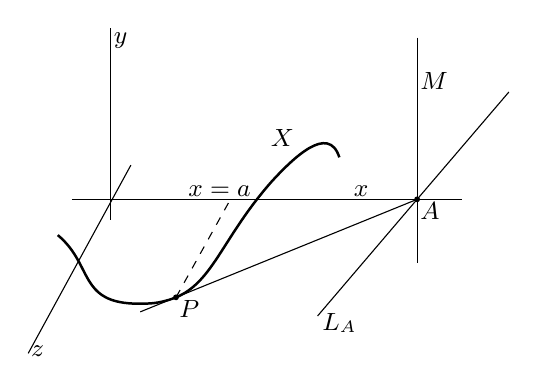
\begin{tikzpicture}[x=.56bp,y=-.56bp,every node/.style={font=\small,inner sep=1pt}]
\draw[thin] (29,111) -- (280,111);
\draw[thin] (54,1) -- (54,124);
\draw[thin] (1,210) -- (67,89);
\draw[thin] (251,7) -- (251,152);
\draw[thin] (187,186) -- (251,111) -- (310,42);
\draw[thin] (73,183.35) -- (96,174) -- (251,111);
\draw[dashed,thin] (96,174) -- (131,111);
\draw[line width=.9pt] (20,134) .. controls (44,154) and (32,180) .. (77,178)
  .. controls (83,178) and (90.1,176.4) .. (96,174)
  .. controls (120,164.2) and (126,135) .. (158,99)
  .. controls (171,85) and (194,62) .. (201,84);
\fill (96,174) circle[radius=1.05bp] node[below right] {$P$};
\fill (251,111) circle[radius=1.05bp] node[below right] {$A$};
\node[above] at (215,111) {$x$};
\node[right] at (54,9) {$y$};
\node[below] at (7,203) {$z$};
\node[above left] at (174,79) {$X$};
\node[right] at (251,35) {$M$};
\node[above] at (124,111) {$x=a$};
\node[below right] at (188,182) {$L_A$};
\end{tikzpicture}\par\nobreak\smallskip
Figure 14.\enspace Proof of \Goto{result-IV-3.9}{(3.9)}.\par}

\medskip
First we project from $A$ to the $yz$-plane.
\EditionText{Since $A$ lies on every tangent line to $X$, the corresponding morphism from $X$ to $\Proj^2$ is ramified everywhere. So either the image is a point (in which case $X$ is a line), or it is inseparable \Goto{result-IV-2.2}{(2.2)}.}
We conclude that the functions $y$ and $z$ restricted to $X$ lie in $K(X)^p$, where $\operatorname{char}k=p>0$.

Next, we project from the $z$-axis to the line $M$ at infinity in the $xy$-plane. In other words, for each point $P\in X$, we define $\varphi(P)$ to be the intersection of the plane spanned by $P$ and the $z$-axis with the line $M$. This gives a morphism $\varphi\colon X\to M$ of degree $d=\deg X$. Note that $\varphi$ is ramified exactly at the points of $X$ which lie in the finite part of the $xz$-plane, but not at $A$.
}
% Contents from body/page-327.tex.
\ChapterSheet{327}{313}{\Goto{sec-IV-3}{3\quad Embeddings in Projective Space}}{%
We will apply Hurwitz's theorem (\Goto{result-IV-2.4}{2.4}) to the morphism $\varphi$. For any point $P\in X\cap xz$-plane, we take $u=x-a$ as a local coordinate, where $a\in k$, $a\ne0$. We take $t=y/x$ as a local coordinate at $A$ on $M$. Then by (\Goto{result-IV-2.2}{2.2}) we have to calculate $v_P(dt/du)$. Write $x=u+a$, so $t=y(u+a)^{-1}$. Since $y\in K(X)^p$, we have $dy/du=0$, so
\[
dt/du=-y(u+a)^{-2}.
\]
\noindent But $u+a$ is a unit in the local ring $\mathcal O_P$, so
\[
v_P(dt/du)=v_P(y).
\]
\noindent If we let $P_1,\ldots,P_r$ be all the finite points of $X\cap xz$-plane, then Hurwitz's theorem tells us that
\[
2g-2=-2d+\sum_{i=1}^r v_{P_i}(y).
\]
Now we consider two cases.

\emph{Case 1.} If $A\notin X$, the $xz$-plane meets $X$ only at the points $P_i$. Since this plane is defined by the equation $y=0$, we can compute the degree of $X$ as the number of intersections of $X$ with this plane, namely
\[
d=\sum_{i=1}^r v_{P_i}(y).
\]
\noindent Substituting in the above, we have
\[
2g-2=-d
\]
\noindent which is possible only if $g=0$ and $d=2$. Thus $X\cong\Proj^1$ as an abstract curve (\Goto{result-IV-1.3.5}{1.3.5}), and its embedding is by a divisor $D$ of degree $2$. We have $\dim|D|=2$ by Riemann--Roch, so $X$ is a conic in a plane $\Proj^2$. \EditionText{For the conic to be strange, we must have $\operatorname{char}k=2$.}

\emph{Case 2.} If $A\in X$, then by condition (\Goto{result-IV-3.9-2}{2}) the $xz$-plane meets $X$ transversally at $A$, so we see similarly
\[
d=\sum_{i=1}^r v_{P_i}(y)+1.
\]
\noindent So
\[
2g-2=-d-1
\]
\noindent which implies $g=0$, $d=1$. This is the line.

\medskip
\noindent\hypertarget{result-IV-3.10}{}\textbf{Theorem 3.10.} \emph{Let $X$ be a curve in $\Proj^3$. Then there is a point $O\notin X$ such that the projection from $O$ determines a birational morphism $\varphi$ from $X$ to its image in $\Proj^2$, and that image has at most nodes for singularities.}

\Proof If $X$ is contained in a plane already, any $O$ not in that plane will do. So we assume $X$ is not contained in any plane. Then in particular, $X$ is
}
% Contents from body/page-328.tex.
\ChapterSheet{328}{314}{\Goto{p-307}{IV\quad Curves}}{%
\noindent neither a line nor a conic, so by (\Goto{result-IV-3.9}{3.9}), $X$ is not strange.
\EditionText{Therefore, by (\Goto{result-IV-3.8}{3.8}), $X$ has a secant which is not a multisecant, and it has a secant without coplanar tangents. Since the same must be true for nearby secants, we see that there is an open subset of $X\times X$ consisting of pairs $\langle P,Q\rangle$ such that the secant line through $P,Q$ is not a multisecant and does not have coplanar tangents. Hence the subset of $X\times X$ consisting of pairs $\langle P,Q\rangle$ where the secant is a multisecant or has coplanar tangents is a proper subset, has dimension $\le1$, and so the union in $\Proj^3$ of the corresponding secant lines has dimension $\le2$.} Combining with the fact that the tangent variety of $X$ has dimension $\le2$ (see (\Goto{result-IV-3.5}{3.5})), we see that there is an open subset of $\Proj^3$ consisting of points $O$ which satisfy (\Goto{result-IV-3.7-2}{2}), (\Goto{result-IV-3.7-3}{3}), and (\Goto{result-IV-3.7-4}{4}) of (\Goto{result-IV-3.7}{3.7}).

To complete the proof, by (\Goto{result-IV-3.7}{3.7}), we must show that $O$ can be chosen to lie on only finitely many secants of $X$. \EditionText{For this we consider the morphism $(X\times X-\Delta)\times\Proj^1\to\Proj^3$ (defined at least locally) which sends $\langle P,Q,t\rangle$ to the point $t$ on the secant line through $P$ and $Q$. If the image has dimension $<3$, then we can choose $O$ lying on no secant. If the image has dimension $=3$, then since it is a morphism between two varieties of the same dimension, we can apply (II, Ex.~\Goto{ex-II-3.7}{3.7}), and find there is an open set of points in $\Proj^3$ over which the fibre is finite.} These points lie on only finitely many secants, so we are done.

\medskip
\noindent\hypertarget{result-IV-3.11}{}\textbf{Corollary 3.11.} \emph{Any curve is birationally equivalent to a plane curve with at most nodes as singularities.}

\Proof Combine (\Goto{result-IV-3.6}{3.6}) with (\Goto{result-IV-3.10}{3.10}).

\medskip
\noindent\hypertarget{result-IV-3.11.1}{}\textbf{Remark 3.11.1.} In view of (\Goto{result-IV-3.11}{3.11}), one way to approach the classification problem for all curves is to study the family of plane curves of degree $d$ with $r$ nodes, for any given $d$ and $r$. The family of all plane curves of degree $d$ is a linear system of dimension $\frac12d(d+3)$, so it is parametrized by a projective space of that dimension. Inside that projective space, the (irreducible) curves with $r$ nodes form a locally closed subset $V_{d,r}$. If $X$ is such a curve, then the genus $g$ of its normalization $\widetilde X$ is given by
\[
g=\tfrac12(d-1)(d-2)-r
\]
\noindent because of (Ex.~\Goto{ex-IV-1.8}{1.8}). So in order for $V_{d,r}$ to be nonempty, we must have
\[
0\le r\le\tfrac12(d-1)(d-2).
\]
\noindent Furthermore, both extremes are possible. We have seen by Bertini's theorem (II, \Goto{result-II-8.20.2}{8.20.2}) that for any $d$, there are irreducible nonsingular curves of degree $d$ in $\Proj^2$, so this gives the case $r=0$. On the other hand, for any $d$, we can embed $\Proj^1$ in $\Proj^d$ as a curve of degree $d$ (Ex.~\Goto{ex-IV-3.4}{3.4}), and then project it into $\Proj^2$ by (\Goto{result-IV-3.5}{3.5}) and (\Goto{result-IV-3.10}{3.10}), to get a curve $X$ of degree $d$ in $\Proj^2$ having only nodes, and with $g(\widetilde X)=0$. This gives $r=\frac12(d-1)(d-2)$.

But the general problem of the structure of the $V_{d,r}$ is very difficult. Severi [\Goto{bib-severi-2}{2}, Anhang F] states that for every $d,r$, satisfying $0\le r\le\frac12(d-1)(d-2)$, the
}
% Contents from body/page-329.tex.
\ChapterSheet{329}{315}{\Goto{sec-IV-3}{3\quad Embeddings in Projective Space}}{%
\noindent algebraic set $V_{d,r}$ is irreducible and nonempty of dimension $\frac12d(d+3)-r$, but a complete proof was given only recently by Joe Harris.

\Exercises
{\fontsize{9}{10.2}\selectfont\setlength{\parskip}{0pt}
\begin{description}[style=multiline,labelwidth=1.9em,leftmargin=2.2em,itemsep=4pt,topsep=0pt,parsep=0pt]
\item[\hypertarget{ex-IV-3.1}{}3.1.] If $X$ is a curve of genus $2$, show that a divisor $D$ is very ample $\Leftrightarrow\deg D\ge5$. This strengthens (\Goto{result-IV-3.3.4}{3.3.4}).
\item[\hypertarget{ex-IV-3.2}{}3.2.] Let $X$ be a plane curve of degree $4$.
\begin{parts}
\item Show that the effective canonical divisors on $X$ are exactly the divisors $X.L$, where $L$ is a line in $\Proj^2$.
\item If $D$ is any effective divisor of degree $2$ on $X$, show that $\dim|D|=0$.
\item Conclude that $X$ is not hyperelliptic (Ex.~\Goto{ex-IV-1.7}{1.7}).
\end{parts}
\item[\hypertarget{ex-IV-3.3}{}3.3.] If $X$ is a curve of genus $\ge2$ which is a complete intersection (II, Ex.~\Goto{ex-II-8.4}{8.4}) in some $\Proj^n$, show that the canonical divisor $K$ is very ample. Conclude that a curve of genus $2$ can never be a complete intersection in any $\Proj^n$. Cf. (Ex.~\Goto{ex-IV-5.1}{5.1}).
\item[\hypertarget{ex-IV-3.4}{}3.4.] Let $X$ be the $d$-uple embedding (I, Ex.~\Goto{ex-I-2.12}{2.12}) of $\Proj^1$ in $\Proj^d$, for any $d\ge1$. We call $X$ the \emph{rational normal curve of degree $d$} in $\Proj^d$.
\begin{parts}
\item Show that $X$ is projectively normal, and that its homogeneous ideal can be generated by forms of degree $2$.
\item If $X$ is any curve of degree $d$ in $\Proj^n$, with $d\le n$, which is not contained in any $\Proj^{n-1}$, show that in fact $d=n$, $g(X)=0$, and $X$ differs from the rational normal curve of degree $d$ only by an automorphism of $\Proj^d$. Cf. (II, \Goto{result-II-7.8.5}{7.8.5}).
\item In particular, any curve of degree $2$ in any $\Proj^n$ is a conic in some $\Proj^2$.
\item A curve of degree $3$ in any $\Proj^n$ must be either a plane cubic curve, or the twisted cubic curve in $\Proj^3$.
\end{parts}
\item[\hypertarget{ex-IV-3.5}{}3.5.] Let $X$ be a curve in $\Proj^3$, which is not contained in any plane.
\begin{parts}
\item If $O\notin X$ is a point, such that the projection from $O$ induces a birational morphism $\varphi$ from $X$ to its image in $\Proj^2$, show that $\varphi(X)$ \emph{must} be singular. [\emph{Hint:} Calculate $\dim H^0(X,\mathcal O_X(1))$ two ways.]
\item If $X$ has degree $d$ and genus $g$, conclude that $g<\frac12(d-1)(d-2)$. (Use (Ex.~\Goto{ex-IV-1.8}{1.8}).)
\item Now let $\{X_t\}$ be the flat family of curves induced by the projection (III, \Goto{result-III-9.8.3}{9.8.3}) whose fibre over $t=1$ is $X$, and whose fibre $X_0$ over $t=0$ is a scheme with support $\varphi(X)$. Show that $X_0$ always has nilpotent elements. Thus the example (III, \Goto{result-III-9.8.4}{9.8.4}) is typical.
\end{parts}
\item[\hypertarget{ex-IV-3.6}{}3.6.] \emph{Curves of Degree 4.}
\begin{parts}
\item If $X$ is a curve of degree $4$ in some $\Proj^n$, show that either
\begin{enumerate}[label=(\arabic*),leftmargin=1.65em,itemsep=0pt,topsep=2pt,parsep=0pt]
\item \EditionText{$g=0$, in which case $X$ is either the rational normal quartic in $\Proj^4$ (Ex.~\Goto{ex-IV-3.4}{3.4}) or the rational quartic curve in $\Proj^3$ (II, \Goto{result-II-7.8.6}{7.8.6}), or}
\item $X\subseteq\Proj^2$, in which case $g=3$, or
\item $X\subseteq\Proj^3$ and $g=1$.
\end{enumerate}
\item In the case $g=1$, show that $X$ is a complete intersection of two irreducible quadric surfaces in $\Proj^3$ (I, Ex.~\Goto{ex-I-5.11}{5.11}). [\emph{Hint:} Use the exact sequence $0\to\mathcal I_X\to\mathcal O_{\Proj^3}\to\mathcal O_X\to0$ to compute $\dim H^0(\Proj^3,\mathcal I_X(2))$, and thus conclude that $X$ is contained in at least two irreducible quadric surfaces.]
\end{parts}
\end{description}
}
}
% Contents from body/page-330.tex.
\ChapterSheet{330}{316}{\Goto{p-307}{IV\quad Curves}}{%
{\fontsize{9}{10.3}\selectfont\setlength{\parskip}{0pt}
\begin{description}[style=multiline,labelwidth=2.55em,leftmargin=2.85em,itemsep=4pt,topsep=0pt,parsep=0pt]
\item[\hypertarget{ex-IV-3.7}{}3.7.] In view of (\Goto{result-IV-3.10}{3.10}), one might ask conversely, is every plane curve with nodes a projection of a nonsingular curve in $\Proj^3$? Show that the curve $xy+x^4+y^4=0$ (assume $\operatorname{char}k\ne2$) gives a counterexample.
\item[\hypertarget{ex-IV-3.8}{}3.8.] We say a (singular) integral curve in $\Proj^n$ is \emph{strange} if there is a point which lies on all the tangent lines at nonsingular points of the curve.
\begin{parts}
\item There are many singular strange curves, e.g., the curve given parametrically by $x=t$, $y=t^p$, $z=t^{2p}$ over a field of characteristic $p>0$.
\item Show, however, that if $\operatorname{char}k=0$, there aren't even any singular strange curves besides $\Proj^1$.
\end{parts}
\item[\hypertarget{ex-IV-3.9}{}3.9.] Prove the following lemma of Bertini: if $X$ is a curve of degree $d$ in $\Proj^3$, not contained in any plane, then for almost all planes $H\subseteq\Proj^3$ (meaning a Zariski open subset of the dual projective space $(\Proj^3)^*$), the intersection $X\cap H$ consists of exactly $d$ distinct points, no three of which are collinear.
\item[\hypertarget{ex-IV-3.10}{}3.10.] Generalize the statement that \textquotedblleft{}not every secant is a multisecant\textquotedblright{} as follows. If $X$ is a curve in $\Proj^n$, not contained in any $\Proj^{n-1}$, and if $\operatorname{char}k=0$, show that for almost all choices of $n-1$ points $P_1,\ldots,P_{n-1}$ on $X$, the linear space $L^{n-2}$ spanned by the $P_i$ does not contain any further points of $X$.
\item[\hypertarget{ex-IV-3.11}{}3.11]
\begin{parts}
\item If $X$ is a nonsingular variety of dimension $r$ in $\Proj^n$, and if $n>2r+1$, show that there is a point $O\notin X$, such that the projection from $O$ induces a closed immersion of $X$ into $\Proj^{n-1}$.
\item If $X$ is the Veronese surface in $\Proj^5$, which is the 2-uple embedding of $\Proj^2$ (I, Ex.~\Goto{ex-I-2.13}{2.13}), show that each point of every secant line of $X$ lies on infinitely many secant lines. Therefore, the secant variety of $X$ has dimension $4$, and so in this case there is a projection which gives a closed immersion of $X$ into $\Proj^4$ (II, Ex.~\Goto{ex-II-7.7}{7.7}). (A theorem of Severi \Goto{bib-severi-1}{[1]} states that the Veronese surface is the only \EditionText{surface} in $\Proj^5$ for which there is a projection giving a closed immersion into $\Proj^4$. Usually one obtains a finite number of double points with transversal tangent planes.)
\end{parts}
\item[\hypertarget{ex-IV-3.12}{}3.12.] For each value of $d=2,3,4,5$ and $r$ satisfying $0\le r\le\frac12(d-1)(d-2)$, show that there exists an irreducible plane curve of degree $d$ with $r$ nodes and no other singularities.
\end{description}
}

\bigskip
\noindent\hypertarget{sec-IV-4}{}\BookMark{1}{4.4  Elliptic Curves}{sec-IV-4}\textbf{\large 4\quad Elliptic Curves}\par\medskip

\noindent The theory of elliptic curves (curves of genus $1$) is varied and rich, and provides a good example of the profound connections between abstract algebraic geometry, complex analysis, and number theory. In this section we will discuss briefly a number of topics concerning elliptic curves, to give some idea of this theory. First we define the $j$-invariant, which classifies elliptic curves up to isomorphism. Then we discuss the group structure on the curve, and show that the elliptic curve is its own Jacobian variety. Next we recall without proof the main results of the theory of elliptic functions of a complex variable, and deduce various results about elliptic curves
}
% Contents from body/page-331.tex.
\ChapterSheet{331}{317}{\Goto{sec-IV-4}{4\quad Elliptic Curves}}{%
\noindent over $\mathbf C$. Then we define the Hasse invariant of a curve over a field of characteristic $p$, and finally we consider the group of rational points of a curve defined over $\mathbf Q$.

For simplicity, we will omit the case of a ground field $k$ of characteristic $2$. Most of the results of this section remain true, but the proofs require special care. See, e.g., Tate \Goto{bib-tate-3}{[3]} or the \textquotedblleft{}formulaire\textquotedblright{} of Deligne and Tate in Birch and Kuyk \Goto{bib-birch-kuyk-1}{[1]}.

\medskip
\emph{The $j$-Invariant}\par
\noindent Our first topic is to define the $j$-invariant of an elliptic curve, and to show that it classifies elliptic curves up to isomorphism. Since $j$ can be any element of the ground field $k$, this will show that the affine line $\AffSpace[k]{1}$ is a variety of moduli for elliptic curves over $k$.

Let $X$ be an elliptic curve over the algebraically closed field $k$. Let $P_0\in X$ be a point, and consider the linear system $|2P_0|$ on $X$. The divisor $2P_0$ is nonspecial, so by Riemann--Roch, this linear system has dimension $1$. It has no base points, because otherwise the curve would be rational. Therefore, it defines a morphism $f\colon X\to\Proj^1$ of degree $2$, and we can specify that $f(P_0)=\infty$ by a change of coordinates in $\Proj^1$.

Now if we assume $\operatorname{char}k\ne2$, it follows from Hurwitz's theorem that $f$ is ramified at exactly four points, with $P_0$ being one of them. If $x=a,b,c$ are the three branch points in $\Proj^1$ besides $\infty$, then there is a unique automorphism of $\Proj^1$ leaving $\infty$ fixed and sending $a$ to $0$ and $b$ to $1$, namely $x'=(x-a)/(b-a)$. So after this automorphism, we may assume that $f$ is branched over the points $0,1,\lambda,\infty$ of $\Proj^1$, where $\lambda\in k$, $\lambda\ne0,1$. This defines a quantity $\lambda$. We define $j=j(\lambda)$ by the formula
\[
j=2^8\frac{(\lambda^2-\lambda+1)^3}{\lambda^2(\lambda-1)^2}.
\]
\noindent This is the $j$-invariant of the curve $X$. (The coefficient $2^8$ is thrown in to make things work in characteristic $2$, despite appearances to the contrary!) Our main result then is the following.

\medskip
\noindent\hypertarget{result-IV-4.1}{}\textbf{Theorem 4.1.} \emph{Let $k$ be an algebraically closed field of characteristic $\ne2$. Then:}
\begin{parts}
\item\hypertarget{result-IV-4.1a}{} \emph{for any elliptic curve $X$ over $k$, the quantity $j$ defined above depends only on $X$;}
\item\hypertarget{result-IV-4.1b}{} \emph{two elliptic curves $X$ and $X'$ over $k$ are isomorphic if and only if $j(X)=j(X')$;}
\item\hypertarget{result-IV-4.1c}{} \emph{every element of $k$ occurs as the $j$-invariant of some elliptic curve over $k$.}
\end{parts}
\emph{Thus we have a one-to-one correspondence between the set of elliptic curves over $k$, up to isomorphism, and the elements of $k$, given by $X\mapsto j(X)$.}
}
% Contents from body/page-332.tex.
\ChapterSheet{332}{318}{\Goto{p-307}{IV\quad Curves}}{%
We will prove this theorem after some other preliminary results.

\medskip
\noindent\hypertarget{result-IV-4.2}{}\textbf{Lemma 4.2.} \emph{Given any two points $P,Q\in X$ (including the case $P=Q$), there is an automorphism $\sigma$ of $X$ such that $\sigma^2=\operatorname{id}$, $\sigma(P)=Q$, and, for any $R\in X$, $R+\sigma(R)\sim P+Q$.}

\Proof The linear system $|P+Q|$ has dimension $1$ and is base-point free, hence defines a morphism $g\colon X\to\Proj^1$ of degree $2$. It is separable, since $X\ncong\Proj^1$ (\Goto{result-IV-2.5}{2.5}), so $K(X)$ is a Galois extension of $K(\Proj^1)$. Let $\sigma$ be the nontrivial automorphism of order $2$ of $K(X)$ over $K(\Proj^1)$. \EditionText{Then $\sigma$ interchanges the two points of each fibre of $g$. Hence $\sigma(P)=Q$, and for any $R\in X$, $R+\sigma(R)$ is a fibre of $g$, hence $R+\sigma(R)\in|P+Q|$, i.e., $R+\sigma(R)\sim P+Q$.}

\medskip
\noindent\hypertarget{result-IV-4.3}{}\textbf{Corollary 4.3.} \emph{The group $\operatorname{Aut}X$ of automorphisms of $X$ is transitive.}

\medskip
\noindent\hypertarget{result-IV-4.4}{}\textbf{Lemma 4.4.} \emph{If $f_1\colon X\to\Proj^1$ and $f_2\colon X\to\Proj^1$ are any two morphisms of degree $2$ from $X$ to $\Proj^1$, then there are automorphisms $\sigma\in\operatorname{Aut}X$ and $\tau\in\operatorname{Aut}\Proj^1$ such that $f_2\circ\sigma=\tau\circ f_1$.}

\begin{center}
\begin{tikzpicture}[x=1cm,y=1cm,>=stealth]
\node (a) at (0,0) {$X$};
\node (b) at (3,0) {$X$};
\node (c) at (0,-1.5) {$\Proj^1$};
\node (d) at (3,-1.5) {$\Proj^1$};
\draw[->,dashed] (a) -- node[above] {$\sigma$} (b);
\draw[->] (a) -- node[left] {$f_1$} (c);
\draw[->] (b) -- node[right] {$f_2$} (d);
\draw[->,dashed] (c) -- node[above] {$\tau$} (d);
\end{tikzpicture}
\end{center}

\Proof Let $P_1\in X$ be a ramification point of $f_1$ and let $P_2\in X$ be a ramification point of $f_2$. Then by (\Goto{result-IV-4.3}{4.3}) there is a $\sigma\in\operatorname{Aut}X$ such that $\sigma(P_1)=P_2$. On the other hand, $f_1$ is determined by the linear system $|2P_1|$ and $f_2$ is determined by $|2P_2|$. Since $\sigma$ takes one to the other, $f_1$ and $f_2\circ\sigma$ correspond to the same linear system, so they differ only by an automorphism $\tau$ of $\Proj^1$ (II, \Goto{result-II-7.8.1}{7.8.1}).

\medskip
\noindent\hypertarget{result-IV-4.5}{}\textbf{Lemma 4.5.} \emph{Let the symmetric group $\Sigma_3$ act on $k-\{0,1\}$ as follows: given $\lambda\in k$, $\lambda\ne0,1$, permute the numbers $0,1,\lambda$ according to $\alpha\in\Sigma_3$, then apply a linear transformation of $x$ to send the first two back to $0,1$, and let $\alpha(\lambda)$ be the image of the third. Then the orbit of $\lambda$ consists of}
\[
\lambda,\frac{1}{\lambda},1-\lambda,\frac{1}{1-\lambda},
\frac{\lambda}{\lambda-1},\frac{\lambda-1}{\lambda}.
\]
\Proof Since the linear transformation sending $a,b$ to $0,1$ is $x'=(x-a)/(b-a)$, we have only to evaluate $(c-a)/(b-a)$, where $\{a,b,c\}=\{0,1,\lambda\}$ in any order.
}
% Contents from body/page-333.tex.
\ChapterSheet{333}{319}{\Goto{sec-IV-4}{4\quad Elliptic Curves}}{%
\noindent\hypertarget{result-IV-4.6}{}\textbf{Proposition 4.6.} \emph{Let $X$ be an elliptic curve over $k$, with $\operatorname{char}k\ne2$, and let $P_0\in X$ be a given point. Then there is a closed immersion $X\to\Proj^2$ such that the image is the curve}
\[
y^2=x(x-1)(x-\lambda)
\]
\noindent\emph{for some $\lambda\in k$, and the point $P_0$ goes to the point at infinity $(0,1,0)$ on the $y$-axis. Furthermore, this $\lambda$ is the same as the $\lambda$ defined earlier, up to an element of $\Sigma_3$ as in \textup{(\Goto{result-IV-4.5}{4.5})}.}

\Proof We embed $X$ in $\Proj^2$ by the linear system $|3P_0|$, which gives a closed immersion (\Goto{result-IV-3.3.3}{3.3.3}). We choose our coordinates as follows. Think of the vector spaces $H^0(\mathcal O(nP_0))$ as contained in each other,
\[
k=H^0(\mathcal O)\subseteq H^0(\mathcal O(P_0))\subseteq H^0(\mathcal O(2P_0))\subseteq\cdots.
\]
\noindent By Riemann--Roch, we have
\[
\dim H^0(\mathcal O(nP_0))=n
\]
\noindent for $n>0$. Choose $x\in H^0(\mathcal O(2P_0))$ so that $1,x$ form a basis of that space, and choose $y\in H^0(\mathcal O(3P_0))$ so that $1,x,y$ form a basis for that space. Then the seven quantities
\[
1,x,y,x^2,xy,x^3,y^2
\]
\noindent are in $H^0(\mathcal O(6P_0))$, which has dimension $6$, so there is a linear relation among them. Furthermore, both $x^3$ and $y^2$ occur with coefficient not equal to zero, because they are the only functions with a 6-fold pole at $P_0$. So replacing $x$ and $y$ by suitable scalar multiples, we may assume they have coefficient $1$. Then we have a relation
\[
y^2+a_1xy+a_3y=x^3+a_2x^2+a_4x+a_6
\]
\noindent for suitable $a_i\in k$.

Now we will make linear changes of coordinates to get the equation in the required form. First we complete the square on the left (here we use $\operatorname{char}k\ne2$), replacing $y$ by
\[
y'=y+\tfrac12(a_1x+a_3).
\]
\noindent The new equation has $y^2$ equal to a cubic equation in $x$, so it can be written
\[
y^2=(x-a)(x-b)(x-c)
\]
\noindent for suitable $a,b,c\in k$. \EditionText{Now we make a linear change of $x$ to send $a,b$ to $0,1$, so the equation becomes
\[
y^2=x(x-1)(x-\lambda)
\]
\noindent as required.}

Since both $x$ and $y$ have a pole at $P_0$, that point goes to the unique point at infinity on this curve, which is $(0,1,0)$.
}
% Contents from body/page-334.tex.
\ChapterSheet{334}{320}{\Goto{p-307}{IV\quad Curves}}{%
If we project from $P_0$ to the $x$-axis, we get a finite morphism of degree $2$, sending $P_0$ to $\infty$, and ramified at $0,1,\lambda,\infty$. So the $\lambda$ is the same as the one defined earlier.

\smallskip
\noindent\textsc{Proof of (\Goto{result-IV-4.1}{4.1}).}\par
(\Goto{result-IV-4.1a}{a}) To show that $j$ depends only on $X$, suppose we made two choices of base point $P_1,P_2\in X$. Let $f_1\colon X\to\Proj^1$ and $f_2\colon X\to\Proj^1$ be the corresponding morphisms. Then by (\Goto{result-IV-4.4}{4.4}) we can find automorphisms $\sigma\in\operatorname{Aut}X$ and $\tau\in\operatorname{Aut}\Proj^1$ such that $f_2\circ\sigma=\tau\circ f_1$. Furthermore, we could choose $\sigma$ such that $\sigma(P_1)=P_2$, hence $\tau(\infty)=\infty$. So $\tau$ sends the branch points $0,1,\lambda_1$ of $f_1$ to the branch points $0,1,\lambda_2$ of $f_2$ in some order. Hence by (\Goto{result-IV-4.5}{4.5}), $\lambda_1$ and $\lambda_2$ differ only by an element of $\Sigma_3$, via the action of (\Goto{result-IV-4.5}{4.5}). So we have only to observe that for any $\alpha\in\Sigma_3$, $j(\lambda)=j(\alpha(\lambda))$. Indeed, since $\Sigma_3$ is generated by any two elements of order $2$, it is enough to show that
\[
j(\lambda)=j\left(\frac1\lambda\right)\qquad\text{and}\qquad j(\lambda)=j(1-\lambda),
\]
\noindent which is clear by direct computation. Thus $j$ depends only on $X$.

(\Goto{result-IV-4.1b}{b}) Now suppose $X$ and $X'$ are two elliptic curves giving rise to $\lambda$ and $\lambda'$, such that $j(\lambda)=j(\lambda')$. First we note that $j$ is a rational function of $\lambda$ of degree $6$, i.e., $\lambda\to j$ defines a finite morphism $\Proj^1\to\Proj^1$ of degree $6$. Furthermore, this is a Galois covering, with Galois group $\Sigma_3$ under the action described above. Therefore, $j(\lambda)=j(\lambda')$ if and only if $\lambda$ and $\lambda'$ differ by an element of $\Sigma_3$.

Now according to (\Goto{result-IV-4.6}{4.6}), $X$ and $X'$ can be embedded in $\Proj^2$ so as to have the equation $y^2=x(x-1)(x-\lambda)$, or same with $\lambda'$. Since $\lambda$ and $\lambda'$ differ by an element of $\Sigma_3$ as in (\Goto{result-IV-4.5}{4.5}), after a linear change of variable in $x$\EditionText{}, we have $\lambda=\lambda'$. Thus $X$ and $X'$ are both isomorphic to the same curve in $\Proj^2$.

(\Goto{result-IV-4.1c}{c}) Given any $j\in k$, we can solve the polynomial equation
\[
2^8(\lambda^2-\lambda+1)^3-j\lambda^2(\lambda-1)^2=0
\]
\noindent for $\lambda$, and find a value of $\lambda$, necessarily $\ne0,1$. Then the equation $y^2=x(x-1)(x-\lambda)$ defines a nonsingular curve of degree $3$ in $\Proj^2$, which is therefore elliptic, and has the given $j$ as its $j$-invariant.

\medskip
\noindent\hypertarget{result-IV-4.6.1}{}\textbf{Example 4.6.1.} The curve $y^2=x^3-x$ of (I, Ex.~\Goto{ex-I-6.2}{6.2}) is nonsingular over any field $k$ with $\operatorname{char}k\ne2$. It has $\lambda=-1$, hence $j=2^6\cdot3^3=1728$.

\medskip
\noindent\hypertarget{result-IV-4.6.2}{}\textbf{Example 4.6.2.} The \textquotedblleft{}Fermat curve\textquotedblright{} $x^3+y^3=z^3$ is nonsingular over any field $k$ with $\operatorname{char}k\ne3$. Making a change of variables $x=x'+z$, and setting $x'=-1/3$, the equation becomes
\[
z^2-\tfrac13z=y^3-\tfrac1{27}.
\]
\noindent From here one can reduce it to a standard form, as in the proof of (\Goto{result-IV-4.6}{4.6}), with $\lambda=-\omega$ or $-\omega^2$, where \EditionText{$\omega^3=1$}. Therefore, $j=0$.
}
% Contents from body/page-335.tex.
\ChapterSheet[10.8]{335}{321}{\Goto{sec-IV-4}{4\quad Elliptic Curves}}{%
\noindent\hypertarget{result-IV-4.7}{}\textbf{Corollary 4.7.} \emph{Let $X$ be an elliptic curve over $k$ with $\operatorname{char}k\ne2$. Let $P_0\in X$, and let $G=\operatorname{Aut}(X,P_0)$ be the group of automorphisms of $X$ leaving $P_0$ fixed. Then $G$ is a finite group of order}
\[
\begin{array}{rl}
2&\textit{if }j\ne0,1728\\
4&\textit{if }j=1728\textit{ and }\operatorname{char}k\ne3\\
6&\textit{if }j=0\textit{ and }\operatorname{char}k\ne3\\
12&\textit{if }j=0\ (=1728)\textit{ and }\operatorname{char}k=3.
\end{array}
\]
\Proof Let $f\colon X\to\Proj^1$ be a morphism of degree $2$, with $f(P_0)=\infty$, branched over $0,1,\lambda,\infty$ as above. If $\sigma\in G$, then by (\Goto{result-IV-4.4}{4.4}) there is an automorphism $\tau$ of $\Proj^1$, sending $\infty$ to $\infty$, such that $f\circ\sigma=\tau\circ f$. In particular, $\tau$ sends $\{0,1,\lambda\}$ to $\{0,1,\lambda\}$ in some order.
\EditionText{If $\tau=\operatorname{id}$, then either $\sigma=\operatorname{id}$ or $\sigma$ is the automorphism interchanging the sheets of $f$. Thus in any case we have two elements in $G$.

If $\tau\ne\operatorname{id}$, then $\tau$ permutes $\{0,1,\lambda\}$, so $\lambda$ must be equal to one of the other expressions of (\Goto{result-IV-4.5}{4.5}). This can happen only in the following cases:}
\begin{enumerate}[label=(\arabic*),leftmargin=1.8em,topsep=3pt,itemsep=1pt]
\item if $\lambda=-1$ or $\frac12$ or $2$, and $\operatorname{char}k\ne3$, then \EditionText{$\lambda$ coincides with one other element of its orbit under $\Sigma_3$}, so $G$ has order $4$. This is the case $j=1728$;
\item if $\lambda=-\omega$ or $-\omega^2$, \EditionText{}and $\operatorname{char}k\ne3$, then \EditionText{$\lambda$ coincides with two other elements of its orbit under $\Sigma_3$}, so $G$ has order $6$. In this case $j=0$;
\item if $\operatorname{char}k=3$ and $\lambda=-1$, then \EditionText{all six elements of the orbit are the same}, so $G$ has order $12$. In this case $j=0=1728$.
\end{enumerate}

\medskip
\emph{The Group Structure}\par
\noindent Let $X$ be an elliptic curve, and let $P_0\in X$ be a fixed point. We have seen, as a consequence of the Riemann--Roch theorem (\Goto{result-IV-1.3.7}{1.3.7}) that the map $P\mapsto\mathcal L(P-P_0)$ induces a bijection between the set of points of $X$ and the group $\operatorname{Pic}^{\circ}X$. Thus the set of points of $X$ forms a group, with $P_0$ as the $0$ element, and with addition characterized by $P+Q=R$ if and only if $P+Q\sim R+P_0$ as divisors on $X$. This is the group structure on $(X,P_0)$.

If we embed $X$ in $\Proj^2$ by the linear system $|3P_0|$, then \EditionText{three points $P,Q,R$ of the image are collinear if and only if $P+Q+R\sim3P_0$.} This in turn is equivalent to saying $P+Q+R=0$ in the group structure. This shows that the group law can be recovered from the geometry of the embedding. It also generalizes (II, \Goto{result-II-6.10.2}{6.10.2}), where we used the geometry to define the group law.

Now we will show that $X$ is a group variety in the sense of (I, Ex.~\Goto{ex-I-3.21}{3.21}).

\medskip
\noindent\hypertarget{result-IV-4.8}{}\textbf{Proposition 4.8.} \emph{Let $(X,P_0)$ be an elliptic curve with its group structure. Then the maps $\rho\colon X\to X$ given by $P\mapsto-P$, and $\mu\colon X\times X\to X$ given by $\langle P,Q\rangle\mapsto P+Q$ are morphisms.}

\Proof First we apply (\Goto{result-IV-4.2}{4.2}) with $P=Q=P_0$. Thus there is an automorphism $\sigma$ of $X$ such that for any $R$, $R+\sigma(R)\sim2P_0$. In other words, $\sigma(R)=-R$ in the group structure, so this $\sigma$ is just $\rho$.
}
% Contents from body/page-336.tex.
\ChapterSheet[10.3]{336}{322}{\Goto{p-307}{IV\quad Curves}}{%
Next we apply (\Goto{result-IV-4.2}{4.2}) to $P$ and $P_0$. So there is an automorphism $\sigma$ of $X$ with $R+\sigma(R)\sim P+P_0$, i.e., $\sigma(R)=P-R$ in the group. Preceding this $\sigma$ with $\rho$, we see that $R\mapsto P+R$, i.e., translation by $P$, is a morphism, for any $P$.

Now take two distinct points $P\ne Q$ in $X$. Embed $X$ in $\Proj^2$ by $|3P_0|$. \EditionText{Form the equation of the line $L$ joining $P$ and $Q$. This depends on the coordinates of $P$ and $Q$. Now intersect $L$ with $X$. We get a cubic equation in the parameter along $L$, but we already know two of the intersections, so we obtain the coordinates of the third point of intersection $R$ as rational functions in the coordinates of $P$ and $Q$. Since $R=-P-Q$ in the group structure, this shows that the map $(X\times X-\Delta)\to X$ defined by $\langle P,Q\rangle\mapsto-P-Q$ is a morphism.} Composing with $\rho$, we see that $\mu$ is a morphism for pairs of distinct points of $X$.

To show that $\mu$ is a morphism also at points of the form $\langle P,P\rangle$, take any $Q\ne0$. Translate one variable by $Q$, apply $\mu$ to $\langle P,P+Q\rangle$, then translate by $-Q$. Since translation is a morphism, we see that $\mu$ is also a morphism at these points.

\medskip
\noindent\hypertarget{result-IV-4.8.1}{}\textbf{Example 4.8.1.} By iterating $\mu$, we see that for any integer $n$, multiplication by $n$ gives a morphism $n_X\colon X\to X$. We will see later that for any $n\ne0$, $n_X$ is a finite morphism of degree $n^2$; \EditionText{its kernel is a group isomorphic to $\mathbf Z/n\times\mathbf Z/n$ if $(n,p)=1$, where $p=\operatorname{char}k$, and is isomorphic to $\mathbf Z/p$ or $0$ if $n=p$, depending on the Hasse invariant of $X$.} See (\Goto{result-IV-4.10}{4.10}), (\Goto{result-IV-4.17}{4.17}), (Ex.~\Goto{ex-IV-4.6}{4.6}), (Ex.~\Goto{ex-IV-4.7}{4.7}), (Ex.~\Goto{ex-IV-4.15}{4.15}).

\medskip
\noindent\hypertarget{result-IV-4.8.2}{}\textbf{Example 4.8.2.} If $P$ is \EditionText{a point of order $2$ on $X$}, then $2P\sim2P_0$, so $P$ is a ramification point of the morphism $f\colon X\to\Proj^1$ defined by $|2P_0|$, and $f$ is separable since $X\ncong\Proj^1$ (\Goto{result-IV-2.5}{2.5}). So there are only finitely many such points, and if $\operatorname{char}k\ne2$, there are exactly $4$. Thus $2_X$ is always a finite morphism, and if $\operatorname{char}k\ne2$, \EditionText{we see that it} has degree $4$, and its kernel \EditionText{}is $\mathbf Z/2\times\mathbf Z/2$.

\medskip
\noindent\hypertarget{result-IV-4.8.3}{}\textbf{Example 4.8.3.} If $P$ is \EditionText{a point of order $3$ on $X$}, then $3P\sim3P_0$, so $P$ is an inflection point of the embedding of $X$ in $\Proj^2$ by $|3P_0|$. If $\operatorname{char}k\ne2,3$, we see by (Ex.~\Goto{ex-IV-2.3}{2.3}) that there are exactly $9$ inflection points of $X$. \EditionText{Thus $3_X$ has degree $9$, and its kernel is isomorphic to $\mathbf Z/3\times\mathbf Z/3$.} By the way, this has the amusing geometric consequence that if $P,Q$ are \EditionText{}inflection points of $X$, then the line $PQ$ meets $X$ in a third inflection point $R$ of $X$. Indeed, $R=-P-Q$, so it is also \EditionText{a point of order $3$}.

\medskip
\noindent\hypertarget{result-IV-4.9}{}\textbf{Lemma 4.9.} \emph{If $X,P_0$ and $X',P'_0$ are two elliptic curves, and if $f\colon X\to X'$ is a morphism sending $P_0$ to $P'_0$, then $f$ is a homomorphism of the group structures.}

\Proof \EditionText{}If $P+Q=R$ on $X$, then $P+Q\sim R+P_0$ as divisors. It follows that $f(P)+f(Q)\sim f(R)+f(P_0)$ by (Ex.~\Goto{ex-IV-2.6}{2.6}), and since $f(P_0)=P'_0$, we have $f(P)+f(Q)=f(R)$ in the group law on $X'$.
}
% Contents from body/page-337.tex.
\ChapterSheet{337}{323}{\Goto{sec-IV-4}{4\quad Elliptic Curves}}{%
\Dfn If $f,g$ are two morphisms of an elliptic curve $X,P_0$ to itself, sending $P_0$ to $P_0$, we define a morphism $f+g$ by composing \EditionText{$f\times g$}$\colon X\to X\times X$ with $\mu$. In other words, $(f+g)(P)=f(P)+g(P)$ for all $P$. We define the morphism $f\cdot g$ to be $f\circ g$. Then the set of all morphisms of $X$ to itself sending $P_0$ to $P_0$ forms a ring $R=\operatorname{End}(X,P_0)$, which we call the \emph{ring of endomorphisms} of $X,P_0$. Its zero element $0$ is the morphism sending $X$ to $P_0$. The unit element $1$ is the identity map. The inverse morphism $\rho$ is $-1$. The distributive law $f\cdot(g+h)=f\cdot g+f\cdot h$ is a consequence of the fact (\Goto{result-IV-4.9}{4.9}) that $f$ is a homomorphism.

\medskip
\noindent\hypertarget{result-IV-4.10}{}\textbf{Proposition 4.10.} \emph{Assume $\operatorname{char}k\ne2$. The map $n\mapsto n_X$ defines an injective ring homomorphism $\mathbf Z\to\operatorname{End}(X,P_0)$. In particular, for all $n\ne0$, $n_X$ is a finite morphism.}

\Proof We will show by induction on $n$ that $n_X\ne0$ for $n\ge1$. It follows that $n_X$ is a finite morphism (II, \Goto{result-II-6.8}{6.8}). For $n=1$ it is clear; for $n=2$ we have seen it above (\Goto{result-IV-4.8.2}{4.8.2}). So let $n>2$. If $n$ is odd, say $n=2r+1$, and if $n_X=0$, then $(2r)_X=\rho$. But $\rho$ has degree $1$, and $(2r)_X=2_X\cdot r_X$ is a finite morphism (use induction hypothesis for $r$) of degree $\ge4$, since $2_X$ has degree $4$ (\Goto{result-IV-4.8.2}{4.8.2}). So this is impossible.

If $n$ is even, say $n=2r$, then $n_X=2_X\cdot r_X$ is finite by induction.

\medskip
\noindent\hypertarget{result-IV-4.10.1}{}\textbf{Remark 4.10.1.} The ring of endomorphisms $R$ is an important invariant of the elliptic curve, but it is not easy to calculate. Let us just note for the moment that its group of units $R^*$ is the group $G=\operatorname{Aut}(X,P_0)$ studied above (\Goto{result-IV-4.7}{4.7}). In particular, if $j=0$ or $1728$, it is bigger than $\{\pm1\}$, so $R$ is definitely bigger than $\mathbf Z$.

\medskip
\emph{The Jacobian Variety}\par
\noindent Now we will give another, perhaps more natural, proof that the group law on the elliptic curve makes it a group variety. Our earlier proof used geometric properties of the embedding in $\Proj^2$. Now instead, we will show that the group $\operatorname{Pic}^{\circ}X$ has a structure of algebraic variety which is so natural that it is automatically a group variety. This approach makes sense for a curve of any genus, and leads to the Jacobian variety of a curve. The idea is to find a universal parameter space for divisor classes of degree $0$.

Let $X$ be a curve over $k$. For any scheme $T$ over $k$, we define $\operatorname{Pic}^{\circ}(X\times T)$ to be the subgroup of $\operatorname{Pic}(X\times T)$ consisting of invertible sheaves whose restriction to each fibre $X_t$ for $t\in T$ has degree $0$. Let $p\colon X\times T\to T$ be the second projection. For any invertible sheaf $\mathcal N$ on $T$, $p^*\mathcal N\in\operatorname{Pic}^{\circ}(X\times T)$, because it is in fact trivial on each fibre. We define $\operatorname{Pic}^{\circ}(X/T)=\operatorname{Pic}^{\circ}(X\times T)/p^*\operatorname{Pic}T$, and we regard its elements as \textquotedblleft{}families of invertible sheaves of degree $0$ on $X$, parametrized by $T$.\textquotedblright{} Justification for this is the fact that if $T$ is integral and of finite type over $k$, and if $\mathcal L,\mathcal M\in\operatorname{Pic}(X\times T)$, then $\mathcal L_t\cong\mathcal M_t$ on $X_t$ for all $t\in T$ if and only if $\mathcal L\otimes\mathcal M^{-1}\in p^*\operatorname{Pic}T$ (III, Ex.~\Goto{ex-III-12.4}{12.4}).
}
% Contents from body/page-338.tex.
\ChapterSheet[10.7]{338}{324}{\Goto{p-307}{IV\quad Curves}}{%
\Dfn Let $X$ be a curve (of any genus) over $k$. The \emph{Jacobian variety} of $X$ is a scheme $J$ of finite type over $k$, together with an element $\mathcal L\in\operatorname{Pic}^{\circ}(X/J)$, having the following universal property: for any scheme $T$ of finite type over $k$, and for any $\mathcal M\in\operatorname{Pic}^{\circ}(X/T)$, there is a unique morphism $f\colon T\to J$ such that $f^*\mathcal L\cong\mathcal M$ in $\operatorname{Pic}^{\circ}(X/T)$. (Note that \EditionText{$f$}$\colon X\times T\to X\times J$ induces a homomorphism $f^*\colon\operatorname{Pic}^{\circ}(X/J)\to\operatorname{Pic}^{\circ}(X/T)$.)

\medskip
\noindent\hypertarget{result-IV-4.10.2}{}\textbf{Remark 4.10.2.} In the language of representable functors, this definition says that $J$ represents the functor $T\to\operatorname{Pic}^{\circ}(X/T)$.

\medskip
\noindent\hypertarget{result-IV-4.10.3}{}\textbf{Remark 4.10.3.} Since $J$ is defined by a universal property, it is unique if it exists. We will prove below that if $X$ is an elliptic curve, then $J$ exists, and in fact we can take $J=X$. For curves of genus $\ge2$ the existence is much more difficult. See, for example, Chow \Goto{bib-chow-3}{[3]} or Mumford \Goto{bib-mumford-2}{[2]} or Grothendieck \Goto{bib-476-5}{[5]}.

\medskip
\noindent\hypertarget{result-IV-4.10.4}{}\textbf{Remark 4.10.4.} Assuming $J$ exists, its closed points are in one-to-one correspondence with elements of the group $\operatorname{Pic}^{\circ}X$. Indeed, to give a closed point of $J$ is the same as giving a morphism $\operatorname{Spec}k\to J$, which by the universal property is the same thing as an element of $\operatorname{Pic}^{\circ}(X/k)=\operatorname{Pic}^{\circ}X$.

\Dfn \EditionText{A scheme $X$ with a morphism to another scheme $S$ is a \emph{group scheme over $S$} if there is a section $e\colon S\to X$ (the identity) and a morphism $\rho\colon X\to X$ over $S$ (the inverse) and a morphism $\mu\colon X\times X\to X$ over $S$ (the group operation) such that
\begin{enumerate}[label=(\arabic*),leftmargin=2.5em,topsep=3pt,itemsep=1pt]
\item\hypertarget{cond-IV-group-inverse}{} the composition $\mu\circ(\operatorname{id}\times\rho)\colon X\to X$ is equal to the projection $X\to S$ followed by $e$, and
\item\hypertarget{cond-IV-group-assoc}{} the two morphisms $\mu\circ(\mu\times\operatorname{id})$ and $\mu\circ(\operatorname{id}\times\mu)$ from $X\times X\times X\to X$ are the same.
\end{enumerate}}

\medskip
\noindent\hypertarget{result-IV-4.10.5}{}\textbf{Remark 4.10.5.} This notion of group scheme generalizes the earlier notion of group variety (I, Ex.~\Goto{ex-I-3.21}{3.21}). Indeed, if $S=\operatorname{Spec}k$ and $X$ is a variety over $k$, taking $e$ to be the $0$ point, \EditionText{the properties (\Goto{cond-IV-group-inverse}{1}), (\Goto{cond-IV-group-assoc}{2}) can be checked on the closed points of $X$. Then (\Goto{cond-IV-group-inverse}{1}) says that $\rho$ gives the inverse of each point, and (\Goto{cond-IV-group-assoc}{2}) says that the group law is associative.}

\medskip
\noindent\hypertarget{result-IV-4.10.6}{}\textbf{Remark 4.10.6.} The Jacobian variety $J$ of a curve $X$ is automatically a group scheme over $k$. Indeed, using the universal property of $J$, define $e\colon\operatorname{Spec}k\to J$ by taking the element $0\in\operatorname{Pic}^{\circ}(X/k)$. Define $\rho\colon J\to J$ by taking $\mathcal L^{-1}\in\operatorname{Pic}^{\circ}(X/J)$. Define $\mu\colon J\times J\to J$ by taking $p_1^*\mathcal L\otimes p_2^*\mathcal L\in\operatorname{Pic}^{\circ}(X/J\times J)$. The \EditionText{properties (\Goto{cond-IV-group-inverse}{1}) and (\Goto{cond-IV-group-assoc}{2})} are verified immediately by the universal property of $J$.

\medskip
\noindent\hypertarget{result-IV-4.10.7}{}\textbf{Remark 4.10.7.} We can determine the Zariski tangent space to $J$ at $0$ as follows. To give an element of the Zariski tangent space is equivalent to
}
% Contents from body/page-339.tex.
\ChapterSheet[10.5]{339}{325}{\Goto{sec-IV-4}{4\quad Elliptic Curves}}{%
\noindent giving a morphism of $T=\operatorname{Spec}k[\varepsilon]/\varepsilon^2$ to $J$ sending $\operatorname{Spec}k$ to $0$ (II, Ex.~\Goto{ex-II-2.8}{2.8}). By the definition of $J$, this is equivalent to giving $\mathcal M\in\operatorname{Pic}^{\circ}(X/T)$ whose restriction to $\operatorname{Pic}^{\circ}(X/k)$ is $0$. But according to (III, Ex.~\Goto{ex-III-4.6}{4.6}) there is an exact sequence $0\to H^1(X,\mathcal O_X)\to\operatorname{Pic}X[\varepsilon]\to\operatorname{Pic}X\to0$. So we see that the Zariski tangent space to $J$ at $0$ is just $H^1(X,\mathcal O_X)$.

\medskip
\noindent\hypertarget{result-IV-4.10.8}{}\textbf{Remark 4.10.8.} $J$ is proper over $k$. We apply the valuative criterion of properness (II, \Goto{result-II-4.7}{4.7}). It is enough to show (II, Ex.~\Goto{ex-II-4.11}{4.11}) that if $R$ is any discrete valuation ring containing $k$, with quotient field $K$, then a morphism of $\operatorname{Spec}K$ to $J$ extends uniquely to a morphism of $\operatorname{Spec}R$ to $J$. In other words, we must show that an invertible sheaf $\mathcal M$ on $X\times\operatorname{Spec}K$ extends uniquely to an invertible sheaf on $X\times\operatorname{Spec}R$. Since $X\times\operatorname{Spec}R$ is a regular scheme, this follows from (II, \Goto{result-II-6.5}{6.5}) (note that the closed fibre of $X\times\operatorname{Spec}R$ over $\operatorname{Spec}R$, as a divisor on $X\times\operatorname{Spec}R$, is linearly equivalent to $0$).

\medskip
\noindent\hypertarget{result-IV-4.10.9}{}\textbf{Remark 4.10.9.} \EditionText{}If we fix a base point $P_0\in X$, then for any $n\ge1$ there is a morphism $\varphi_n\colon X^n\to J$ defined by \textquotedblleft{}$\langle P_1,\ldots,P_n\rangle\mapsto\mathcal L(P_1+\cdots+P_n-nP_0)$\textquotedblright{} (which means cook up the appropriate sheaf on $X\times X^n$ to define $\varphi_n$). If $g$ is the genus of $X$, then $\varphi_n$ will be surjective for $n\ge g$, because by Riemann--Roch, every divisor class of degree $\ge g$ contains an effective divisor. The fibre of $\varphi_n$ over a point of $J$ consists of all $n$-tuples $\langle P_1,\ldots,P_n\rangle$ such that the divisors $P_1+\cdots+P_n$ form a complete linear system.

If $n=g$, then for most choices of $P_1,\ldots,P_g$, we have $l(P_1+\cdots+P_g)=1$. Indeed, by Riemann--Roch,
\[
l(P_1+\cdots+P_g)=g+1-g+l(K-P_1-\cdots-P_g).
\]
\noindent But $l(K)=g$. Taking $P_1$ not a base point of $K$, $l(K-P_1)=g-1$. At each step, taking $P_i$ not a base point of $K-P_1-\cdots-P_{i-1}$, we get $l(K-P_1-\cdots-P_g)=0$. Therefore, most fibres of $\varphi_g$ are finite sets of points. We conclude that $J$ is irreducible and $\dim J=g$. On the other hand, by (\Goto{result-IV-4.10.7}{4.10.7}), the Zariski tangent space to $J$ at $0$ is $H^1(X,\mathcal O_X)$, which has dimension $g$, so $J$ is nonsingular at $0$. \EditionText{Since it is a group scheme, it is a homogeneous space, hence nonsingular everywhere.} Hence $J$ is a nonsingular variety.

\medskip
\noindent\hypertarget{result-IV-4.11}{}\textbf{Theorem 4.11.} \emph{Let $X$ be an elliptic curve, and fix a point $P_0\in X$. Take $J=X$, and take $\mathcal L$ on $X\times J$ to be $\mathcal L(\Delta)\otimes p_1^*\mathcal L(-P_0)$, where $\Delta\subseteq X\times X$ is the diagonal. Then $J,\mathcal L$ is a Jacobian variety for $X$. Furthermore, the resulting structure of group variety on $J$ \textup{(\Goto{result-IV-4.10.6}{4.10.6})} induces the same group structure on $X,P_0$ as defined earlier.}

\Proof The last statement is obvious from the definitions. So we have only to show that if $T$ is any scheme of finite type over $k$, and if $\mathcal M\in\operatorname{Pic}^{\circ}(X/T)$, then there is a unique morphism $f\colon T\to J$ such that $f^*\mathcal L\cong\mathcal M$.

Let $p\colon X\times T\to T$ be the projection, and let $q\colon X\times T\to X$ be the other projection. Define $\mathcal M'=\mathcal M\otimes q^*\mathcal L(P_0)$. Then $\mathcal M'$ has degree $1$ along the fibres. Hence, for any closed point $t\in T$, we can apply Riemann--Roch to
}
% Contents from body/page-340.tex.
\ChapterSheet[10.3]{340}{326}{\Goto{p-307}{IV\quad Curves}}{%
\noindent $\mathcal M'_t$ on $X_t=X$, and we find
\[
\begin{aligned}
\dim H^0(X,\mathcal M'_t)&=1\\
\dim H^1(X,\mathcal M'_t)&=0.
\end{aligned}
\]
Since $p$ is a projective morphism, and $\mathcal M'$ is flat over $T$, we can apply the theorem of cohomology and base change (III, \Goto{result-III-12.11}{12.11}). Looking first at $R^1p_*(\mathcal M')$, since the cohomology along the fibres is $0$, the map $\varphi^1(t)$ of (III, \Goto{result-III-12.11}{12.11}) is automatically surjective, hence an isomorphism, so we conclude that $R^1p_*(\mathcal M')$ is identically $0$. In particular, it is locally free, so we deduce from part (\Goto{result-III-12.11b}{b}) of the theorem that $\varphi^0(t)$ is also surjective. Therefore, it is an isomorphism, and since $\varphi^{-1}(t)$ is always surjective, we see that $p_*(\mathcal M')$ is locally free of rank $1$.

Now replacing $\mathcal M$ by $\mathcal M\otimes p^*p_*(\mathcal M')^{-1}$ in $\operatorname{Pic}^{\circ}(X/T)$, we may then assume that $p_*(\mathcal M')\cong\mathcal O_T$. The section $1\in\Gamma(T,\mathcal O_T)$ gives a section $s\in\Gamma(X\times T,\mathcal M')$, \EditionText{which defines an effective Cartier divisor $Z\subseteq X\times T$. By construction, $Z$ intersects each fibre of $p$ in just one point, and in fact one sees easily that the restricted morphism $p\colon Z\to T$ is an isomorphism.} Thus we get a section $s\colon T\to Z\subseteq X\times T$. Composing with $q$ gives the required morphism $f\colon T\to X$.

Indeed, since $Z$ is the graph of $f$, we see that $Z=f^*\Delta$, where $\Delta\subseteq X\times X$ is the diagonal. Hence the corresponding invertible sheaves correspond: $\mathcal M'\cong f^*\mathcal L(\Delta)$. Now twisting by $-P_0$ shows that $\mathcal M\cong f^*\mathcal L$, as required. The uniqueness of $f$ is clear for the same reasons.

\medskip
\emph{Elliptic Functions}\par
\noindent It is hard to discuss elliptic curves without bringing in the theory of elliptic functions of a complex variable. This classical topic from complex analysis gives an insight into the theory of elliptic curves over $\mathbf C$ which cannot be matched by purely algebraic techniques. So we will recall some of the definitions and results of that theory without proof (signaling those statements with a B in their number), and give some applications to elliptic curves. We refer to the book Hurwitz--Courant \Goto{bib-hurwitz-courant-1}{[1]} for proofs.

Fix a complex number $\tau$, $\tau\notin\mathbf R$. Let $\Lambda$ be the lattice in the complex plane $\mathbf C$ consisting of all $n+m\tau$, with $n,m\in\mathbf Z$ (Fig.~\Goto{fig-book-15}{15}).

\begin{center}
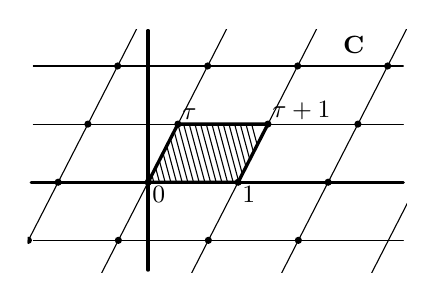
\begin{tikzpicture}[x=.9cm,y=.9cm,line cap=round,font=\small]
\begin{scope}
\clip (-1.7,-1.27) rectangle (3.65,2.15);
\foreach \m in {-1,1,2}{\draw (-1.62,{.82*\m})--(3.6,{.82*\m});}
\foreach \n in {-1,0,1,2,3}{\draw ({1.27*\n+.42*(-1.45)/.82},-1.45)--({1.27*\n+.42*2.2/.82},2.2);}
\draw[very thick] (-1.65,0)--(3.6,0) (0,-1.24)--(0,2.14);
\begin{scope}
\clip (0,0)--(1.27,0)--(1.69,.82)--(.42,.82)--cycle;
\foreach \t in {0,.08,...,1.76}{\draw[thin] (\t,0)--({\t-.22},.82);}
\end{scope}
\draw[very thick] (0,0)--(1.27,0)--(1.69,.82)--(.42,.82)--cycle;
\foreach \n in {-1,0,1,2}{\foreach \m in {-1,0,1,2}{\fill ({1.27*\n+.42*\m},{.82*\m}) circle[radius=1.3pt];}}
\end{scope}
\node[below right,inner sep=1.3pt] at (0,0) {$0$};
\node[below right,inner sep=1.3pt] at (1.27,0) {$1$};
\node[above right,inner sep=1.4pt] at (.42,.82) {$\tau$};
\node[above right,inner sep=1.4pt] at (1.69,.82) {$\tau+1$};
\node at (2.9,1.93) {$\mathbf C$};
\end{tikzpicture}\\[3pt]
\small\hypertarget{fig-book-15}{}Figure 15.\quad A lattice in $\mathbf C$, with one period parallelogram.
\end{center}
}
% Contents from body/page-341.tex.
\ChapterSheet{341}{327}{\Goto{sec-IV-4}{4\quad Elliptic Curves}}{%
\Dfn An \emph{elliptic function} (with respect to the lattice $\Lambda$) is a meromorphic function $f(z)$ of the complex variable $z$ such that $f(z+\omega)=f(z)$ for all $\omega\in\Lambda$. (Sometimes these are called \emph{doubly periodic functions}, since they are periodic with respect to the periods $1,\tau$.)

\smallskip
Because of the periodicity, an elliptic function is determined if one knows its values on a single \emph{period parallelogram}, such as the one bounded by $0,1,\tau,\tau+1$ (Fig.~\Goto{fig-book-15}{15}).

An example of an elliptic function is the \emph{Weierstrass $\wp$-function} defined by
\[
\wp(z)=\frac1{z^2}+\sum_{\omega\in\Lambda'}\left(\frac1{(z-\omega)^2}-\frac1{\omega^2}\right),
\]
\noindent where $\Lambda'=\Lambda-\{0\}$. One shows (Hurwitz--Courant [\Goto{bib-hurwitz-courant-1}{1}, II, 1, \S6]) that this series converges at all $z\notin\Lambda$, thus giving a meromorphic function having a double pole at the points of $\Lambda$, and which is elliptic. Its derivative
\[
\wp'(z)=\sum_{\omega\in\Lambda}\frac{-2}{(z-\omega)^3}
\]
\noindent is another elliptic function.

If one adds, subtracts, multiplies, or divides two elliptic functions with periods in $\Lambda$, one gets another such. Hence the elliptic functions for a given $\Lambda$ form a field.

\medskip
\noindent\hypertarget{result-IV-4.12B}{}\textbf{Theorem 4.12B.} \emph{The field of elliptic functions for given $\Lambda$ is generated over $\mathbf C$ by the Weierstrass $\wp$-function and its derivative $\wp'$. They satisfy the algebraic relation}
\[
(\wp')^2=4\wp^3-g_2\wp-g_3,
\]
\noindent\emph{where}
\[
g_2=60\sum_{\omega\in\Lambda'}\frac1{\omega^4}\qquad\textit{and}\qquad
g_3=140\sum_{\omega\in\Lambda'}\frac1{\omega^6}.
\]
\Proof Hurwitz--Courant [\Goto{bib-hurwitz-courant-1}{1}, II, 1, \S\S8, 9].

\smallskip
Thus if we define a mapping $\varphi\colon\mathbf C\to\Proj^2_{\mathbf C}$ by sending $z\to(\wp(z),\wp'(z))$ in affine coordinates, we obtain a holomorphic mapping whose image lies inside the curve $X$ with equation
\[
y^2=4x^3-g_2x-g_3.
\]
\noindent In fact, $\varphi$ induces a bijective mapping of $\mathbf C/\Lambda$ to $X$ (Hurwitz--Courant [\Goto{bib-hurwitz-courant-1}{1}, II, 5, \S1]), and $X$ is nonsingular, hence an elliptic curve. Under this mapping the field of elliptic functions is identified with the function field of the curve $X$. Thus for any elliptic function, we can speak of its \emph{divisor} $\sum n_i(a_i)$, with $a_i\in\mathbf C/\Lambda$.
}
% Contents from body/page-342.tex.
\ChapterSheet{342}{328}{\Goto{p-307}{IV\quad Curves}}{%
\noindent\hypertarget{result-IV-4.13B}{}\textbf{Theorem 4.13B.} \emph{Given distinct points $a_1,\ldots,a_q\in\mathbf C/\Lambda$, and given integers $n_1,\ldots,n_q$, a necessary and sufficient condition that there exist an elliptic function with divisor $\sum n_i(a_i)$ is that $\sum n_i=0$ and $\sum n_i a_i=0$ in the group $\mathbf C/\Lambda$.}

\Proof Hurwitz--Courant [\Goto{bib-hurwitz-courant-1}{1}, II, 1, \S\S5, 14].

\smallskip
In particular, this says that $a_1+a_2\equiv b\pmod\Lambda$ if and only if there is an elliptic function \EditionText{with zeros at $a_1$ and $a_2$, and poles at $b$ and $0$.} Since this function is a rational function on the curve $X$, this says that $\varphi(a_1)+\varphi(a_2)\sim\varphi(b)+\varphi(0)$ as divisors on $X$. If we let $P_0=\varphi(0)$, which is the point at infinity on the $y$-axis, and give $X$ the group structure with origin $P_0$, this says that $\varphi(a_1)+\varphi(a_2)=\varphi(b)$ in the group structure on $X$. In other words, $\varphi$ gives a group isomorphism between $\mathbf C/\Lambda$ under addition, and $X$ with its group law.

\medskip
\noindent\hypertarget{result-IV-4.14B}{}\textbf{Theorem 4.14B.} \emph{Given $c_2,c_3\in\mathbf C$, with $\Delta\ne0$, where $\Delta=c_2^3-27c_3^2$, there exists a $\tau\in\mathbf C$, $\tau\notin\mathbf R$, and an $\alpha\in\mathbf C$, $\alpha\ne0$, such that the lattice $\Lambda=(1,\tau)$ gives $g_2=\alpha^4c_2$ and $g_3=\alpha^6c_3$ by the formulas above.}

\Proof Hurwitz--Courant [\Goto{bib-hurwitz-courant-1}{1}, II, 4, \S4].

\smallskip
This shows that every elliptic curve over $\mathbf C$ arises in this way. Indeed, if $X$ is any elliptic curve, we can embed $X$ in $\Proj^2$ to have an equation of the form $y^2=x(x-1)(x-\lambda)$, with $\lambda\ne0,1$ (\Goto{result-IV-4.6}{4.6}). By a linear change of variable in $x$, one can bring this into the form $y^2=4x^3-c_2x-c_3$, with $c_2=(\sqrt[3]{4}/3)(\lambda^2-\lambda+1)$ and $c_3=(1/27)(\lambda+1)(2\lambda^2-5\lambda+2)$. Then $\Delta=\lambda^2(\lambda-1)^2$, which is $\ne0$ since $\lambda\ne0,1$. Now the curve determined by the lattice $\Lambda$ is equivalent to this one by a change of variables $y'=\alpha^3 y$, $x'=\alpha^2x$.

Next we define $J(\tau)=g_2^3/\Delta$. Then the $j$-invariant of $X$ which we defined earlier is just $j=1728\cdot J(\tau)$. Thus $J(\tau)$ classifies the curve $X$ up to isomorphism.

\medskip
\noindent\hypertarget{result-IV-4.15B}{}\textbf{Theorem 4.15B.} \emph{Let $\tau,\tau'$ be two \EditionText{complex numbers}. Then $J(\tau)=J(\tau')$ if and only if there are integers $a,b,c,d\in\mathbf Z$ with $ad-bc=\pm1$ and}
\[
\tau'=\frac{a\tau+b}{c\tau+d}.
\]
\noindent\emph{Furthermore, given any $\tau'$, there is a unique $\tau$ with $J(\tau)=J(\tau')$ such that $\tau$ lies in the region $G$ \textup{(Fig.~\Goto{fig-book-16}{16})} defined by}
\[
\EditionText{}
-\tfrac12\le\operatorname{Re}\tau<\tfrac12
\]
\noindent\emph{and}
\[
\begin{array}{ll}
|\tau|\ge1&\textit{if }\operatorname{Re}\tau\le0\\
|\tau|>1&\textit{if }\operatorname{Re}\tau>0.
\end{array}
\]
}
% Contents from body/page-343.tex.
\ChapterSheet[10.8]{343}{329}{\Goto{sec-IV-4}{4\quad Elliptic Curves}}{%
\begin{center}
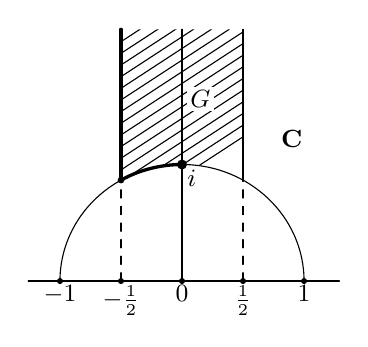
\begin{tikzpicture}[x=1.55cm,y=1.48cm,line cap=round,font=\small]
\begin{scope}
\clip (-.5,{sqrt(3)/2}) arc[start angle=120,end angle=60,radius=1] -- (.5,2.16)--(-.5,2.16)--cycle;
\foreach \t in {.54,.64,...,2.68}{\draw[thin] (-.52,\t)--(1.03,{\t+1.06});}
\end{scope}
\draw (-1.26,0)--(1.29,0) (0,0)--(0,2.16);
\draw (-1,0) arc[start angle=180,end angle=0,x radius=1,y radius=1];
\draw[dashed] (-.5,0)--(-.5,{sqrt(3)/2}) (.5,0)--(.5,{sqrt(3)/2});
\draw[very thick] (-.5,2.16)--(-.5,{sqrt(3)/2});
\draw[very thick] (-.5,{sqrt(3)/2}) arc[start angle=120,end angle=90,x radius=1,y radius=1];
\draw[thin] (.5,{sqrt(3)/2})--(.5,2.16);
\fill (0,1) circle[radius=1.8pt] (-.5,{sqrt(3)/2}) circle[radius=1.2pt];
\foreach \x/\lab in {-1/{-1},-.5/{-\frac12},0/{0},.5/{\frac12},1/{1}}{
  \fill (\x,0) circle[radius=1.1pt];
  \node[below,inner sep=1.5pt] at (\x,0) {$\lab$};
}
\node[below right,inner sep=1.7pt] at (0,1) {$i$};
\node[fill=white,inner sep=1.3pt] at (.15,1.56) {$G$};
\node at (.9,1.22) {$\mathbf C$};
\end{tikzpicture}\\[3pt]
\small\hypertarget{fig-book-16}{}Figure 16.\quad The region $G$.
\end{center}

\Proof Hurwitz--Courant [\Goto{bib-hurwitz-courant-1}{1}, II, 4, \S3].

\smallskip
Now we will start drawing consequences from this theory.

\medskip
\noindent\hypertarget{result-IV-4.16}{}\textbf{Theorem 4.16.} \emph{Let $X$ be an elliptic curve over $\mathbf C$. Then as an abstract group, $X$ is isomorphic to $\mathbf R/\mathbf Z\times\mathbf R/\mathbf Z$. In particular, \EditionText{for any $n$, the subgroup of points of order $n$} is isomorphic to $\mathbf Z/n\times\mathbf Z/n$.}

\Proof We have seen that $X$ is isomorphic as a group to $\mathbf C/\Lambda$, which in turn is isomorphic to $\mathbf R/\mathbf Z\times\mathbf R/\mathbf Z$. The points of order \EditionText{$n$} are represented by $(a/n)+(b/n)\tau$, with $a,b=0,1,\ldots,n-1$. The points whose coordinates are not rational combinations of $1,\tau$ are of infinite order.

\medskip
\noindent\hypertarget{result-IV-4.17}{}\textbf{Corollary 4.17.} \emph{The morphism multiplication by $n$\EditionText{}, $n_X\colon X\to X$, is a finite morphism of degree $n^2$.}

\Proof Since it is separable, and a group homomorphism, its degree is the order of the kernel, which is $n^2$.

\smallskip
Next we will investigate the ring of endomorphisms $R=\operatorname{End}(X,P_0)$ of the elliptic curve $X$ determined by the elliptic functions with periods $1,\tau$.

\medskip
\noindent\hypertarget{result-IV-4.18}{}\textbf{Proposition 4.18.} \emph{There is a one-to-one correspondence between endomorphisms $f\in R$ and complex numbers $\alpha\in\mathbf C$ such that $\alpha\cdot\Lambda\subseteq\Lambda$. This correspondence gives an injective ring homomorphism of $R$ to $\mathbf C$.}

\Proof Given $f\in R$, we have seen (\Goto{result-IV-4.9}{4.9}) that $f$ is a group homomorphism of $X$ to $X$. \EditionText{Hence under the identification of $X$ with $\mathbf C/\Lambda$ it gives a group homomorphism $\bar f$ of $\mathbf C$ to $\mathbf C$, such that $\bar f(\Lambda)\subseteq\Lambda$. On the other hand, since $f$ is a morphism, the induced map $\bar f\colon\mathbf C\to\mathbf C$ is holomorphic. Now expanding $\bar f$ as a power series in a neighborhood of the origin, and expressing the fact that $\bar f(z+w)=\bar f(z)+\bar f(w)$ for any $z,w$ there, we see that $\bar f$ must be just multiplication by some complex number $\alpha$.}
}
% Contents from body/page-344.tex.
\ChapterSheet{344}{330}{\Goto{p-307}{IV\quad Curves}}{%
Conversely, given $\alpha\in\mathbf C$, such that $\alpha\cdot\Lambda\subseteq\Lambda$, clearly multiplication by $\alpha$ induces a group homomorphism $f$ of $\mathbf C/\Lambda$ to itself, hence of $X$ to itself. But $f$ is also holomorphic, so in fact it is a morphism of $X$ to itself by GAGA ($=$ Serre \Goto{bib-serre-4}{[4]}): see (App.~\Goto{p-452}{B}, Ex.~\Goto{ex-B-6.6}{6.6}).

It is clear under this correspondence that the ring operations of $R$ correspond to addition and multiplication of the corresponding complex numbers $\alpha$.

\medskip
\noindent\hypertarget{result-IV-4.18.1}{}\textbf{Remark 4.18.1.} Note in particular that the morphism $n_X\in R$, which is multiplication by $n$ in the group structure (\Goto{result-IV-4.8.1}{4.8.1}) corresponds to multiplication by $n$ in $\mathbf C$. This gives another proof of (\Goto{result-IV-4.10}{4.10}) for elliptic curves over $\mathbf C$.

\Dfn If $X$ is an elliptic curve over $\mathbf C$, we say it has \emph{complex multiplication} if the ring of endomorphisms $R$ is bigger than $\mathbf Z$. This terminology is explained by (\Goto{result-IV-4.18}{4.18}).

\medskip
\noindent\hypertarget{result-IV-4.19}{}\textbf{Theorem 4.19.} \emph{If $X$ has complex multiplication, then $\tau\in\mathbf Q(\sqrt{-d})$ for some $d\in\mathbf Z$, $d>0$, and in that case, $R$ is a subring $(\ne\mathbf Z)$ of the ring of integers of the field $\mathbf Q(\sqrt{-d})$. Conversely, if $\tau=r+s\sqrt{-d}$, with $r,s\in\mathbf Q$, then $X$ has complex multiplication, and in fact}
\[
R=\{a+b\tau\mid a,b\in\mathbf Z,\text{ and }2br,b(r^2+ds^2)\in\mathbf Z\}.
\]
\Proof Given $\tau$, we can determine $R$ as the set of all $\alpha\in\mathbf C$ such that $\alpha\cdot\Lambda\subseteq\Lambda$. A necessary and sufficient condition for $\alpha\cdot\Lambda\subseteq\Lambda$ is that there exist integers $a,b,c,e$ such that
\[
\begin{aligned}
\alpha&=a+b\tau\\
\alpha\tau&=c+e\tau.
\end{aligned}
\]
\noindent If $\alpha\in\mathbf R$, then $\alpha\in\mathbf Z$, so we see that $R\cap\mathbf R=\mathbf Z$. On the other hand, if $X$ has complex multiplication, then there is an $\alpha\notin\mathbf R$, and in this case, $b\ne0$.

Eliminating $\alpha$ from these equations, we see that
\[
b\tau^2+(a-e)\tau-c=0,
\]
\noindent which shows that $\tau$ is in a quadratic extension of $\mathbf Q$. Since $\tau\notin\mathbf R$, it must be an imaginary quadratic extension, so $\tau\in\mathbf Q(\sqrt{-d})$ for some $d\in\mathbf Z$, $d>0$.

Eliminating $\tau$ from the same equations, we find
\[
\alpha^2-(\EditionText{a-e})\alpha+(ae-bc)=0,
\]
\noindent which shows that $\alpha$ is integral over $\mathbf Z$. Therefore $R$ must be a subring of the ring of integers of the field $\mathbf Q(\sqrt{-d})$.

Conversely, suppose $\tau=r+s\sqrt{-d}$, with $r,s\in\mathbf Q$. Then we can determine $R$ as the set of all $\alpha=a+b\tau$, with $a,b\in\mathbf Z$, such that $\alpha\tau\in\Lambda$. Since
}
% Contents from body/page-345.tex.
\ChapterSheet{345}{331}{\Goto{sec-IV-4}{4\quad Elliptic Curves}}{%
\noindent $\alpha\tau=a\tau+b\tau^2$, we must have $b\tau^2\in\Lambda$. Now
\[
\tau^2=r^2-ds^2+2rs\sqrt{-d},
\]
\noindent which can be written
\[
\tau^2=-(r^2+ds^2)+2r\tau.
\]
\noindent So in order to have $b\tau^2\in\Lambda$ we must have $2br\in\mathbf Z$ and $b(r^2+ds^2)\in\mathbf Z$. These conditions are necessary and sufficient so we get the required expression for $R$. In particular, $R>\mathbf Z$, so $X$ has complex multiplication.

\medskip
\noindent\hypertarget{result-IV-4.20}{}\textbf{Corollary 4.20.} \emph{There are only countably many values of $j\in\mathbf C$ for which the corresponding elliptic curve $X$ has complex multiplication.}

\Proof Indeed, there are only countably many elements of all quadratic extensions of $\mathbf Q$.

\medskip
\noindent\hypertarget{result-IV-4.20.1}{}\textbf{Example 4.20.1.} If $\tau=i$, then $R$ is the ring of Gaussian integers $\mathbf Z[i]$. In this case the group of units $R^*$ of $R$ consists of $\pm1,\pm i$, so $R^*\cong\mathbf Z/4$. This means that the group \EditionText{of automorphisms of $X$} has order $4$, so by (\Goto{result-IV-4.7}{4.7}) we must have $j=1728$. So we see in a roundabout way that $\tau=i$ gives $J(\tau)=1$. Another way to see this is as follows. Since $\Lambda=\mathbf Z\oplus\mathbf Zi$, the lattice $\Lambda$ is stable under multiplication by $i$. Therefore
\[
g_3=140\sum_{\omega\in\Lambda'}\omega^{-6}
 =140\sum_{\omega\in\Lambda'}i^{-6}\omega^{-6}=-g_3.
\]
\noindent So $g_3=0$, which implies that $J(\tau)=1$. The equation of $X$ can be written $y^2=x^3-Ax$.

\medskip
\noindent\hypertarget{result-IV-4.20.2}{}\textbf{Example 4.20.2.} If $\tau=\omega$, where $\omega^3=1$, then $R=\mathbf Z[\omega]$, which is the ring of integers in the field $\mathbf Q(\sqrt{-3})$. In this case $R^*=\{\pm1,\pm\omega,\pm\omega^2\}$ which is isomorphic to $\mathbf Z/6$. So again from (\Goto{result-IV-4.7}{4.7}) we conclude that $j=0$. One can also see this directly as in (\Goto{result-IV-4.20.1}{4.20.1}) by showing that $g_2=0$. The equation of $X$ can be written $y^2=x^3-B$.

\medskip
\noindent\hypertarget{result-IV-4.20.3}{}\textbf{Example 4.20.3.} If $\tau=2i$, then $R=\mathbf Z[2i]$. In this case $R$ is a proper subring of the ring of integers in the quadratic field $\mathbf Q(i)$, with conductor $2$ (Ex.~\Goto{ex-IV-4.21}{4.21}).

\medskip
\noindent\hypertarget{result-IV-4.20.4}{}\textbf{Remark 4.20.4.} Even though we have a good criterion for complex multiplication in terms of $\tau$, the connection between $\tau$ and $j$ is not easy to compute. Thus if we are given a curve by its equation in $\Proj^2$, or by its $j$-invariant, it is not easy to tell whether it has complex multiplication or not. See (Ex.~\Goto{ex-IV-4.5}{4.5}) and (Ex.~\Goto{ex-IV-4.12}{4.12}). There is an extensive classical literature relating complex multiplication to class field theory---see, e.g., Deuring \Goto{bib-deuring-2}{[2]} or Serre's article in Cassels and Fr\"ohlich [\Goto{bib-cassels-frohlich-1}{1}, Ch.~XIII]. Here are some of the principal results: let $X$ be an elliptic curve with complex multiplication, let $R=\operatorname{End}(X,P_0)$,
}
% Contents from body/page-346.tex.
\ChapterSheet[10.8]{346}{332}{\Goto{p-307}{IV\quad Curves}}{%
\noindent let $K=\mathbf Q(\sqrt{-d})$ be the quotient field of $R$ (\Goto{result-IV-4.19}{4.19}), and let $j$ be the $j$-invariant. Then (1) $j$ is an algebraic integer; (2) the field $K(j)$ is an abelian extension of $K$ of degree $h_R=\#\operatorname{Pic}R$; (3) $j\in\mathbf Z\Leftrightarrow h_R=1$, and there are exactly $13$ such values of $j$.

\medskip
\emph{The Hasse Invariant}\par
\noindent If $X$ is an elliptic curve over a field $k$ of characteristic $p>0$, we define an important invariant of $X$ as follows. Let $F\colon X\to X$ be the Frobenius morphism (\Goto{result-IV-2.4.1}{2.4.1}). Then $F$ induces a map
\[
F^*\colon H^1(X,\mathcal O_X)\longrightarrow H^1(X,\mathcal O_X)
\]
\noindent on cohomology. \EditionText{This map is not linear, but it is \emph{$p$-linear}, namely $F^*(\lambda a)=\lambda^p F^*(a)$ for all $\lambda\in k$, $a\in H^1(X,\mathcal O_X)$.} Since $X$ is elliptic, $H^1(X,\mathcal O_X)$ is a one-dimensional vector space. Thus, since $k$ is perfect, the map $F^*$ is either $0$ or bijective.

\Dfn If $F^*=0$, we say that $X$ has \emph{Hasse invariant} $0$ or that $X$ is \emph{supersingular}; otherwise we say that $X$ has \emph{Hasse invariant} $1$.

\smallskip
For other interpretations of the Hasse invariant, see (Ex.~\Goto{ex-IV-4.15}{4.15}), (Ex.~\Goto{ex-IV-4.16}{4.16}).

\medskip
\noindent\hypertarget{result-IV-4.21}{}\textbf{Proposition 4.21.} \emph{Let the elliptic curve $X$ be embedded as a cubic curve in $\Proj^2$ with homogeneous equation $f(x,y,z)=0$. Then the Hasse invariant of $X$ is $0$ if and only if the coefficient of $(xyz)^{p-1}$ in $f^{p-1}$ is $0$.}

\Proof The ideal sheaf of $X$ is isomorphic to $\mathcal O_{\Proj}(-3)$, so we have an exact sequence
\[
0\longrightarrow\mathcal O_{\Proj}(-3)\xrightarrow{f}\mathcal O_{\Proj}\longrightarrow\mathcal O_X\longrightarrow0.
\]
\noindent From this, by taking cohomology, we obtain an isomorphism
\[
H^1(X,\mathcal O_X)\longrightarrow H^2(\mathcal O_{\Proj}(-3)),
\]
\noindent since $H^i(\mathcal O_{\Proj})=0$ for $i=1,2$. Recall also (III, \Goto{result-III-5.1}{5.1}) that $H^2(\mathcal O_{\Proj}(-3))$ is a one-dimensional vector space with a natural basis $(xyz)^{-1}$.

Now we can compute the action of Frobenius using this embedding. If $F_1$ is the Frobenius morphism on $\Proj^2$, then $F_1^*$ takes $\mathcal O_X$ to $\mathcal O_{X^p}$, where $X^p$ is the subscheme of $\Proj^2$ defined by $f^p=0$. On the other hand, $X$ is a closed subscheme of $X^p$, so we have a commutative diagram
\begin{center}
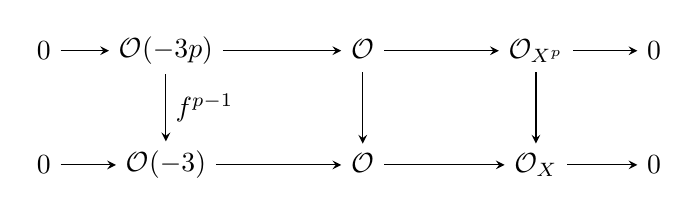
\begin{tikzpicture}[>=stealth,x=1cm,y=1cm]
\node (a) at (0,0) {$0$};
\node (b) at (1.55,0) {$\mathcal O_{\Proj}(-3p)$};
\node (c) at (4.05,0) {$\mathcal O_{\Proj}$};
\node (d) at (6.25,0) {$\mathcal O_{X^p}$};
\node (e) at (7.75,0) {$0$};
\node (f) at (0,-1.45) {$0$};
\node (g) at (1.55,-1.45) {$\mathcal O_{\Proj}(-3)$};
\node (h) at (4.05,-1.45) {$\mathcal O_{\Proj}$};
\node (i) at (6.25,-1.45) {$\mathcal O_X$};
\node (j) at (7.75,-1.45) {$0$};
\draw[->] (a)--(b);\draw[->] (b)--(c);\draw[->] (c)--(d);\draw[->] (d)--(e);
\draw[->] (f)--(g);\draw[->] (g)--(h);\draw[->] (h)--(i);\draw[->] (i)--(j);
\draw[->] (b)--node[right]{$f^{p-1}$}(g);\draw[->] (c)--(h);\draw[->] (d)--(i);
\end{tikzpicture}
\end{center}
}
% Contents from body/page-347.tex.
\ChapterSheet[10.7]{347}{333}{\Goto{sec-IV-4}{4\quad Elliptic Curves}}{%
\noindent Hence we have a commutative diagram
\begin{center}
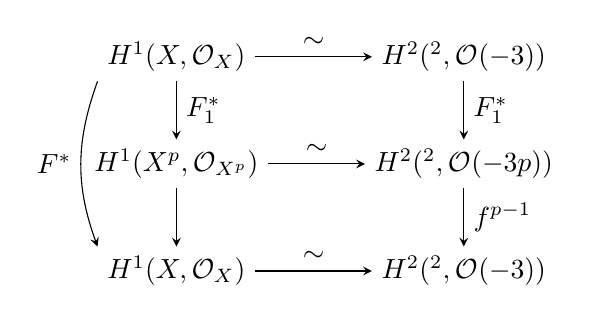
\begin{tikzpicture}[>=stealth,x=1cm,y=1cm]
\node (a) at (0,0) {$H^1(X,\mathcal O_X)$};
\node (b) at (3.65,0) {$H^2(\Proj^2,\mathcal O_{\Proj}(-3))$};
\node (c) at (0,-1.36) {$H^1(X^p,\mathcal O_{X^p})$};
\node (d) at (3.65,-1.36) {$H^2(\Proj^2,\mathcal O_{\Proj}(-3p))$};
\node (e) at (0,-2.72) {$H^1(X,\mathcal O_X)$};
\node (f) at (3.65,-2.72) {$H^2(\Proj^2,\mathcal O_{\Proj}(-3))$};
\draw[->] (a)--node[above]{$\sim$}(b);\draw[->] (c)--node[above]{$\sim$}(d);\draw[->] (e)--node[above]{$\sim$}(f);
\draw[->] (a)--node[right]{$F_1^*$}(c);\draw[->] (b)--node[right]{$F_1^*$}(d);
\draw[->] (c)--(e);\draw[->] (d)--node[right]{$f^{p-1}$}(f);
\draw[->] (a.south west) to[bend right=20] node[left]{$F^*$} (e.north west);
\end{tikzpicture}
\end{center}

\noindent where $F$ is the Frobenius morphism of $X$. Now $F_1^*((xyz)^{-1})=(xyz)^{-p}$, and its image in $H^2(\mathcal O_{\Proj}(-3))$ will be $f^{p-1}\cdot(xyz)^{-p}$. On the other hand, $H^2(\mathcal O_{\Proj}(-3))$ has basis $(xyz)^{-1}$, and any monomial having a nonnegative exponent on $x,y$, or $z$ is $0$. Thus the image is just $(xyz)^{-1}$ times the coefficient of $(xyz)^{p-1}$ in $f^{p-1}$, and so the Hasse invariant of $X$ is determined by whether or not this coefficient is zero.

\medskip
\noindent\hypertarget{result-IV-4.22}{}\textbf{Corollary 4.22.} \emph{Assume $p\ne2$, and let $X$ be given by the equation $y^2=x(x-1)(x-\lambda)$, with $\lambda\ne0,1$. Then the Hasse invariant of $X$ is $0$ if and only if $h_p(\lambda)=0$, where}
\[
h_p(\lambda)=\sum_{i=0}^k\binom{k}{i}^{\!2}\lambda^i,\qquad
k=\tfrac12(p-1).
\]
\Proof We use the criterion of (\Goto{result-IV-4.21}{4.21}). In this case $f=y^2z-x(x-z)(x-\lambda z)$. To get $(xyz)^{p-1}$ in $f^{p-1}$, we must have $(y^2z)^k$ and $(x(x-z)(x-\lambda z))^k$. Then, inside $((x-z)(x-\lambda z))^k$, we need the coefficient of $x^kz^k$. So we take the coefficient of $x^iz^{k-i}$ in $(x-z)^k$, and the coefficient of $x^{k-i}z^i$ in $(x-\lambda z)^k$. \EditionText{Summing up, the coefficient of $(xyz)^{p-1}$ in $f^{p-1}$ is
\[
(-1)^k\binom{p-1}{k}\sum\binom{k}{i}^{\!2}\lambda^i.
\]
\noindent Since the outer factor is $\equiv1\pmod p$, we get $h_p(\lambda)$ as defined above.}

\medskip
\noindent\hypertarget{result-IV-4.23}{}\textbf{Corollary 4.23.} \emph{For given $p$, there are only finitely many elliptic curves (up to isomorphism) over $k$ having Hasse invariant $0$. In fact, there are at most $\lfloor p/12\rfloor+2$ of them.}

\Proof The polynomial $h_p(\lambda)$ has degree $k=\frac12(p-1)$ in $\lambda$, so it has at most $k$ distinct roots. In particular, there are only finitely many corresponding values of $j$. \EditionText{Since the correspondence $\lambda\mapsto j$ is $6$ to $1$ with two exceptions, we can have at most $k/6+2$ values of $j$, hence at most $\lfloor p/12\rfloor+2$.}
}
% Contents from body/page-348.tex.
\ChapterSheet{348}{334}{\Goto{p-307}{IV\quad Curves}}{%
\noindent\emph{Note.} In fact, Igusa \Goto{bib-478-5}{[2]} has shown that the roots of $h_p(\lambda)$ are always distinct. Using this, one can easily count the exact number of $j$ with Hasse invariant $0$: \EditionText{}$j=0$ occurs $\Leftrightarrow p\equiv2\pmod3$ (Ex.~\Goto{ex-IV-4.14}{4.14}); $j=1728$ occurs $\Leftrightarrow p\equiv3\pmod4$ (\Goto{result-IV-4.23.5}{4.23.5}); the number of $j\ne0,1728$ is exactly $[p/12]$. \EditionText{}There are also tables of these $j$ for small values of $p$---see Deuring \Goto{bib-475-9}{[1]} or Birch and Kuyk \Goto{bib-birch-kuyk-1}{[1, Table~6]}.

\medskip
\noindent\hypertarget{result-IV-4.23.1}{}\textbf{Example 4.23.1.} Let $p=3$. Then $h_p(\lambda)=\lambda+1$. The only solution is $\lambda=-1$, which corresponds to $j=0=1728$.

\medskip
\noindent\hypertarget{result-IV-4.23.2}{}\textbf{Example 4.23.2.} If $p=5$, $h_p(\lambda)=\lambda^2+4\lambda+1\equiv\lambda^2-\lambda+1\pmod5$. This has roots $-\omega,-\omega^2$ in a quadratic extension of $\mathbb F_p$, with \EditionText{$\omega^3=1$}. So $j=0$.

\medskip
\noindent\hypertarget{result-IV-4.23.3}{}\textbf{Example 4.23.3.} If $p=7$, then
\[
h_p(\lambda)=\lambda^3+9\lambda^2+9\lambda+1.
\]
This has roots $-1,2,4$, which correspond to $j=1728$.

\medskip
\noindent\hypertarget{result-IV-4.23.4}{}\textbf{Remark 4.23.4.} A very interesting problem arises if we \textquotedblleft{}fix the curve and vary $p$.\textquotedblright{} To make sense of this, let $X\subseteq\mathbf P_{\mathbb C}^2$ be a cubic curve defined by an equation $f(x,y,z)=0$ with integer coefficients, and assume that $X$ is nonsingular as a curve over $\mathbb C$. Then for almost all primes $p$, the curve $X_{(p)}\subseteq\mathbf P_{\mathbb F_p}^2$ obtained by reducing the coefficients of $f$ (mod $p$) will be nonsingular over $k_{(p)}=\mathbb F_p$. So it makes sense to consider the set
{\small
\[
\mathfrak P=\{p\ \text{prime}\mid X_{(p)}\text{ is nonsingular over }k_{(p)},\text{ and }X_{(p)}\text{ has Hasse invariant }0\}.
\]}
What can we say about this set? The facts (which we will not prove) are that if $X$, as a curve over $\mathbb C$, has complex multiplication, then $\mathfrak P$ has density $\frac12$. Here we define the \emph{density} of a set of primes $\mathfrak P$ to be
\[
\lim_{x\to\infty}\#\{p\in\mathfrak P\mid p\le x\}/\#\{p\ \text{prime}\mid p\le x\}.
\]
In fact, assuming $X_{(p)}$ is nonsingular, then $X_{(p)}$ has Hasse invariant $0$ if and only if either $p$ is ramified or $p$ remains prime in the imaginary quadratic field containing the ring of complex multiplication of $X$ (Deuring \Goto{bib-475-9}{[1]}). If $X$ does not have complex multiplication, then $\mathfrak P$ has density $0$, but Elkies has shown that $\mathfrak P$ is infinite (N. Elkies, The existence of infinitely many supersingular primes for every elliptic curve over $\mathbb Q$, Invent.\ Math.\ 89 (1987) 561--567). There is also ample numerical evidence for the conjecture of Lang and Trotter \Goto{bib-479-3-item-1}{[1]}, that more precisely
\[
\#\{p\in\mathfrak P\mid p\le x\}\sim c\cdot\sqrt{x}/\log x
\]
as $x\to\infty$, for some constant $c>0$.

\medskip
\noindent\hypertarget{result-IV-4.23.5}{}\textbf{Example 4.23.5.} Let $X$ be the curve $y^2=x^3-x$. Then $j=1728$, and as we have seen (\Goto{result-IV-4.20.1}{4.20.1}), $X$ has complex multiplication by $i$. For any $p\ne2$, $X_{(p)}$ is nonsingular, and we compute its Hasse invariant by the criterion of (\Goto{result-IV-4.21}{4.21}). With $k=\frac12(p-1)$, we need the coefficient of $x^k$ in $(x^2-1)^k$. If $k$ is}
% Contents from body/page-349.tex.
\ChapterSheet{349}{335}{\Goto{sec-IV-4}{4\quad Elliptic Curves}}{%
\noindent odd, it is $0$. If $k$ is even, say $k=2m$, it is $(-1)^m\binom{k}{m}$ which is nonzero. We conclude that
\[
\begin{cases}
\text{if }p\equiv1\pmod4,\text{ then Hasse}=1\\
\text{if }p\equiv3\pmod4,\text{ then Hasse}=0.
\end{cases}
\]
Thus $\mathfrak P=\{p\ \text{prime}\mid p\equiv3\pmod4\}$. According to Dirichlet's theorem on primes in arithmetic progressions (see, e.g., Serre \Goto{bib-serre-14}{[14, Ch.~VI, \S4]}), this is a set of primes of density $\frac12$. In particular, there are infinitely many such primes. Note that $p\equiv3\pmod4$ if and only if $p$ is prime in the ring of Gaussian integers $\mathbb Z[i]$.

\medskip
\noindent\hypertarget{result-IV-4.23.6}{}\textbf{Example 4.23.6.} Let $X$ be the curve $y^2=x(x-1)(x+2)$, so $\lambda=-2$, and $j=2^6\cdot3^{-2}\cdot7^3$. Then $X_{(p)}$ is nonsingular for $p\ne2,3$, but one checks by the criterion of (\Goto{result-IV-4.22}{4.22}), using a calculator, that the only value of $p\le73$ giving Hasse $=0$ is $p=23$. So we can guess that $\mathfrak P$ has density $0$. Indeed, $j$ is not an integer, so by (\Goto{result-IV-4.20.4}{4.20.4}), $X$ does not have complex multiplication. See Lang and Trotter \Goto{bib-479-3-item-1}{[1]} for more extensive computations.

\medskip
\noindent\emph{Rational Points on an Elliptic Curve}\par
\smallskip
Let $X$ be an elliptic curve over an algebraically closed field $k$, let $P_0$ be a fixed point, and let $X$ be embedded in $\mathbf P_k^2$ by the linear system $|3P_0|$. Suppose that $X$ can be defined by an equation $f(x,y,z)=0$ with coefficients in a smaller field $k_0\subseteq k$, and that the point $P_0$ has coordinates in $k_0$. In this case we say $(X,P_0)$ is \emph{defined over $k_0$}. If this happens, then it is clear from the geometric nature of the group law on $X$, that the set $X(k_0)$ of points of $X$ with coordinates in $k_0$ forms a subgroup of the group of all points of $X$. It is an interesting arithmetic problem to determine the nature of this subgroup.

In particular, if $k=\mathbb C$ and $k_0=\mathbb Q$, then because $x,y,z$ are homogeneous coordinates in $\mathbf P^2$, we may assume that the equation $f(x,y,z)=0$ has integer coefficients, and we are looking for integer solutions $x,y,z$. So we have a cubic Diophantine equation in three variables.

A theorem of Mordell states that the group $X(\mathbb Q)$ is a finitely generated abelian group. We will not prove this, but just give some examples. See Cassels \Goto{bib-474-11-item-1}{[1]} and Tate \Goto{bib-tate-3}{[3]} for two excellent surveys of the subject.

\medskip
\noindent\hypertarget{result-IV-4.23.7}{}\textbf{Example 4.23.7.} The Fermat curve $x^3+y^3=z^3$ is defined over $\mathbb Q$. Because Fermat's theorem is true for exponent $3$, the only points of $X(\mathbb Q)$ are $(1,-1,0)$, $(1,0,1)$, and $(0,1,1)$. These are three inflection points of $X$. Taking any one as base point, the group $X(\mathbb Q)$ is isomorphic to $\mathbb Z/3$.

\medskip
\noindent\hypertarget{result-IV-4.23.8}{}\textbf{Example 4.23.8.} The curve $y^2+y=x^3-x$ is defined over $\mathbb Q$. Take $P_0=(0,1,0)$ to be the $0$ element in the group law, as usual. Then (according to Tate \Goto{bib-tate-3}{[3]}), the group $X(\mathbb Q)$ is infinite cyclic, generated by the point $P$ with affine coordinates $(0,0)$. Figure~\Goto{fig-book-17}{17} shows this curve, with $nP$ labeled as $n$, for various integers~$n$.}
% Contents from body/page-350.tex.
\ChapterSheet{350}{336}{\Goto{p-307}{IV\quad Curves}}{%
\fontsize{9.5}{10.4}\selectfont%
\setlength{\parskip}{0pt}%
\setlength{\smallskipamount}{1.8pt}%
\setlength{\medskipamount}{3.6pt}%
\setlength{\abovedisplayskip}{3.2pt}%
\setlength{\belowdisplayskip}{3.2pt}%
{\centering
\hypertarget{fig-book-17}{}%
\resizebox{.70\linewidth}{!}{%
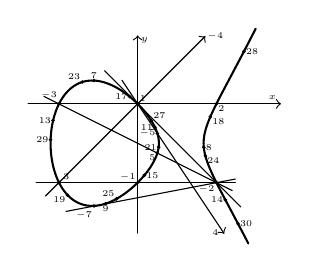
\begin{tikzpicture}[x=1cm,y=1cm,line cap=round,line join=round,
  every node/.style={font=\tiny,inner sep=.55pt},
  point three/.style={above right,xshift=.85pt,yshift=.25pt},
  point minus two/.style={below left,yshift=-.45pt},
  point minus three/.style={above left,yshift=1.0pt},
  point minus seven/.style={below left,yshift=-1.25pt}]
  \draw[->] (-1.39,0)--(1.82,0) node[above left,xshift=-1.1pt,yshift=.7pt] {\scalebox{.64}{$x$}};
  \draw[->] (0,-1.64)--(0,.87) node[below right,xshift=.5pt] {\scalebox{.64}{$y$}};
  \draw[thin] (-1.29,-1)--(1.24,-1);
  \draw[thin,->] (-1.17,-1.17)--(.86,.86) node[right] {\scalebox{.64}{$-4$}};
  \draw[thin,->] (-.20,.30)--(1.10,-1.65) node[left,xshift=-1.35pt,yshift=.35pt] {\scalebox{.64}{$4$}};
  \draw[thin] (-1.19,.095)--(1.20,-1.10);
  \draw[thin] (-.91,-1.366)--(1.24,-.955);
  \draw[thin] (-.42,.42)--(1.31,-1.31);
  \draw[line width=.75pt,domain=0:360,samples=150,smooth,variable=\t]
    plot ({-.418452+.688051*cos(\t)}, {-.5+sin(\t)*.688051*sqrt(max(0,.837565-(-.418452+.688051*cos(\t))))});
  \draw[line width=.75pt,domain=0:1.15,samples=100,smooth,variable=\t]
    plot ({.837565+.50*\t^2}, {-.5+\t*sqrt(max(0,.50*(.837565+.50*\t^2+1.106681)*(.837565+.50*\t^2-.269594)))});
  \draw[line width=.75pt,domain=0:1.065,samples=100,smooth,variable=\t]
    plot ({.837565+.50*\t^2}, {-.5-\t*sqrt(max(0,.50*(.837565+.50*\t^2+1.106681)*(.837565+.50*\t^2-.269594)))});
  \foreach \x/\y/\pointlabel/\where in {
      0/0/1/above right, 0/-1/-1/above left,
      1/0/2/below right, 1/-1/-2/point minus two,
      -1/-1/3/point three, -1/0/-3/point minus three,
      .25/-.625/5/below left, .25/-.375/-5/left,
      -.555556/.296296/7/above, -.555556/-1.296296/-7/point minus seven,
      .84/-.552/8/right, -.408163/-1.268222/9/below,
      .219282/-.296869/11/left, -1.074691/-.211098/13/left,
      1.113274/-1.218676/14/left, .085044/-.906904/15/right,
      -.102567/.092864/17/left, .922317/-.164933/18/below right,
      -.890339/-1.159215/19/below left, .266391/-.550129/21/left,
      -.704051/.277857/23/above left, .859803/-.660674/24/below right,
      -.269362/-1.206978/25/above left, .173486/-.214105/27/above right,
      1.349612/.665607/28/right, -1.106381/-.454350/29/left,
      1.275025/-1.523607/30/right}
  {%
    \fill (\x,\y) circle[radius=.7pt];
    \node[\where] at (\x,\y) {\scalebox{.64}{$\pointlabel$}};
  }
\end{tikzpicture}}\par
\smallskip
\small\textbf{Figure 17.}\enspace Rational points on the curve $y^2+y=x^3-x$.\par
}
\medskip
\noindent\textsc{Exercises}

\smallskip
\noindent\hypertarget{ex-IV-4.1}{}\textbf{4.1.} Let $X$ be an elliptic curve over $k$, with $\operatorname{char}k\ne2$, let $P\in X$ be a point, and let $R$ be the graded ring $R=\bigoplus_{n\ge0}H^0(X,\mathcal O_X(nP))$. Show that for suitable choice of $t,x,y$,
\[
R\cong k[t,x,y]/(y^2-x(x-t^2)(x-\lambda t^2)),
\]
as a graded ring, where $k[t,x,y]$ is graded by setting $\deg t=1$, $\deg x=2$, $\deg y=3$.

\smallskip
\noindent\hypertarget{ex-IV-4.2}{}\textbf{4.2.} If $D$ is any divisor of degree $\ge3$ on the elliptic curve $X$, and if we embed $X$ in $\mathbf P^n$ by the complete linear system $|D|$, show that the image of $X$ in $\mathbf P^n$ is projectively normal.

\emph{Note.} It is true more generally that if $D$ is a divisor of degree $\ge2g+1$ on a curve of genus $g$, then the embedding of $X$ by $|D|$ is projectively normal (Mumford \Goto{bib-mumford-4}{[4, p.~55]}).

\smallskip
\noindent\hypertarget{ex-IV-4.3}{}\textbf{4.3.} Let the elliptic curve $X$ be embedded in $\mathbf P^2$ so as to have the equation $y^2=x(x-1)(x-\lambda)$. Show that any automorphism of $X$ leaving $P_0=(0,1,0)$ fixed is induced by an automorphism of $\mathbf P^2$ coming from the automorphism of the affine $(x,y)$-plane given by
\[
\begin{cases}
x'=ax+b\\
y'=cy.
\end{cases}
\]
In each of the four cases of (\Goto{result-IV-4.7}{4.7}), describe these automorphisms of $\mathbf P^2$ explicitly, and hence determine the structure of the group $G=\operatorname{Aut}(X,P_0)$.

\smallskip
\noindent\hypertarget{ex-IV-4.4}{}\textbf{4.4.} Let $X$ be an elliptic curve in $\mathbf P^2$ given by an equation of the form
\[
y^2+a_1xy+a_3y=x^3+a_2x^2+a_4x+a_6.
\]
\EditionText{Show that the $j$-invariant is a rational function of the $a_i$, with coefficients in $\mathbb Q$.} In particular, if the $a_i$ are all in some field $k_0\subseteq k$, then $j\in k_0$ also. Furthermore,}
% Contents from body/page-351.tex.
\ChapterSheet[10.6]{351}{337}{\Goto{sec-IV-4}{4\quad Elliptic Curves}}{%
\fontsize{9.15}{9.85}\selectfont%
\setlength{\parskip}{0pt}%
\setlength{\smallskipamount}{1.5pt}%
\setlength{\medskipamount}{3.6pt}%
\setlength{\abovedisplayskip}{3.2pt}%
\setlength{\belowdisplayskip}{3.2pt}%
\noindent for every $\alpha\in k_0$, there exists an elliptic curve defined over $k_0$ with $j$-invariant equal to $\alpha$.

\smallskip
\noindent\hypertarget{ex-IV-4.5}{}\textbf{4.5.} \EditionText{}Let $X,P_0$ be an elliptic curve having an endomorphism $f\colon X\to X$ of degree $2$.

\noindent\hangindent=2.6em\hspace*{1.4em}(a) If we represent $X$ as a $2$-$1$ covering of $\mathbf P^1$ by a morphism $\pi\colon X\to\mathbf P^1$ ramified at $P_0$, then as in (\Goto{result-IV-4.4}{4.4}), show that there is another morphism $\pi'\colon X\to\mathbf P^1$ and a morphism $g\colon\mathbf P^1\to\mathbf P^1$, also of degree $2$, such that $\pi\circ f=g\circ\pi'$.

\noindent\hangindent=2.6em\hspace*{1.4em}(b) For suitable choices of coordinates in the two copies of $\mathbf P^1$, show that $g$ can be taken to be the morphism $x\mapsto x^2$.

\noindent\hangindent=2.6em\hspace*{1.4em}(c) Now show that $g$ is branched over two of the branch points of $\pi$, and that $g^{-1}$ of the other two branch points of $\pi$ consists of the four branch points of $\pi'$. Deduce a relation involving the invariant $\lambda$ of $X$.

\noindent\hangindent=2.6em\hspace*{1.4em}(d) Solving the above, show that there are just three values of $j$ corresponding to elliptic curves with an endomorphism of degree $2$, and find the corresponding values of $\lambda$ and $j$. [\emph{Answers:} $j=2^6\cdot3^3$; $j=2^6\cdot5^3$; $j=-3^3\cdot5^3$.]

\smallskip
\noindent\hypertarget{ex-IV-4.6}{}\textbf{4.6.} \EditionText{}(a) Let $X$ be a curve of genus $g$ embedded birationally in $\mathbf P^2$ as a curve of degree $d$ with $r$ nodes. Generalize the method of (Ex.~\Goto{ex-IV-2.3}{2.3}) to show that \EditionText{$X$ has $6(g-1)+3d$ inflection points. A node does not count as an inflection point. Assume $\operatorname{char}k=0$.}

\noindent\hangindent=2.6em\hspace*{1.4em}(b) Now let $X$ be a curve of genus $g$ embedded as a curve of degree $d$ in $\mathbf P^n$, $n\ge3$, not contained in any $\mathbf P^{n-1}$. For each point $P\in X$, there is a hyperplane $H$ containing $P$, such that $P$ counts at least $n$ times in the intersection $H\cap X$. This is called an \emph{osculating hyperplane} at $P$. It generalizes the notion of tangent line for curves in $\mathbf P^2$. If $P$ counts at least $n+1$ times in $H\cap X$, we say $H$ is a \emph{hyperosculating hyperplane}, and that $P$ is a \emph{hyperosculation point}. Use Hurwitz's theorem as above, and induction on $n$, to show that $X$ has $n(n+1)(g-1)+(n+1)d$ hyperosculation points\EditionText{}.

\noindent\hangindent=2.6em\hspace*{1.4em}(c) If $X$ is an elliptic curve, for any $d\ge3$, embed $X$ as a curve of degree $d$ in $\mathbf P^{d-1}$, and conclude that $X$ has exactly $d^2$ points of order \EditionText{$d$} in its group law.

\smallskip
\noindent\hypertarget{ex-IV-4.7}{}\textbf{4.7.} \emph{The Dual of a Morphism.} Let $X$ and $X'$ be elliptic curves over $k$, with base points $P_0,P'_0$.

\noindent\hangindent=2.6em\hspace*{1.4em}(a) If $f\colon X\to X'$ is any morphism, use (\Goto{result-IV-4.11}{4.11}) to show that $f^*\colon\operatorname{Pic}X'\to\operatorname{Pic}X$ induces a homomorphism $\widehat f\colon(X',P'_0)\to(X,P_0)$. We call this the \emph{dual} of $f$.

\noindent\hangindent=2.6em\hspace*{1.4em}(b) If $f\colon X\to X'$ and $g\colon X'\to X''$ are two morphisms, then $(g\circ f)^\wedge=\widehat f\circ\widehat g$.

\noindent\hangindent=2.6em\hspace*{1.4em}(c) Assume $f(P_0)=P'_0$\EditionText{}, and let $n=\deg f$. Show that if $Q\in X$ is any point, and $f(Q)=Q'$, then $\widehat f(Q')=n_X(Q)$. (Do the separable and purely inseparable cases separately, then combine.) Conclude that $f\circ\widehat f=n_{X'}$ and $\widehat f\circ f=n_X$.

\noindent\hangindent=2.6em\hspace*{1.1em}*(d) If $f,g\colon X\to X'$ are two morphisms preserving the base points $P_0,P'_0$, then $(f+g)^\wedge=\widehat f+\widehat g$. [\emph{Hints:} It is enough to show for any $\mathcal L\in\operatorname{Pic}\EditionText{}X'$, that $(f+g)^*\mathcal L\cong f^*\mathcal L\otimes g^*\mathcal L$. For any $f$, let $\Gamma_f\colon X\to X\times X'$ be the graph morphism. Then it is enough to show (for $\mathcal L'=p_2^*\mathcal L$) that
\[
\Gamma_{f+g}^*(\mathcal L')=\Gamma_f^*\mathcal L'\otimes\Gamma_g^*\mathcal L'.
\]
Let $\sigma\colon X\to X\times X'$ be the section $x\mapsto(x,P'_0)$. Define a subgroup of $\operatorname{Pic}(X\times X')$ as follows:
\[
\begin{aligned}
\operatorname{Pic}_\sigma^0=\{&\mathcal L\in\operatorname{Pic}(X\times X')\mid
  \mathcal L\text{ has degree }0\text{ along each fibre of }p_1,\\
 &\text{and }\sigma^*\mathcal L=0\text{ in }\operatorname{Pic}X\}.
\end{aligned}
\]}
% Contents from body/page-352.tex.
\ChapterSheet[10.7]{352}{338}{\Goto{p-307}{IV\quad Curves}}{%
\fontsize{9.5}{10.25}\selectfont%
\setlength{\parskip}{0pt}%
\setlength{\smallskipamount}{1.65pt}%
\setlength{\medskipamount}{3.6pt}%
\setlength{\abovedisplayskip}{3.2pt}%
\setlength{\belowdisplayskip}{3.2pt}%
\noindent Note that this subgroup is isomorphic to the group $\operatorname{Pic}^0(X'/X)$ used in the definition of the Jacobian variety. Hence there is a $1$-$1$ correspondence between morphisms $f\colon X\to X'$ and elements $\mathcal L_f\in\operatorname{Pic}_\sigma^0$ (this defines $\mathcal L_f$).

Now compute explicitly to show that $\Gamma_g^*(\mathcal L_f)=\Gamma_f^*(\mathcal L_g)$ for any $f,g$.

Use the fact that $\mathcal L_{f+g}=\mathcal L_f\otimes\mathcal L_g$, and the fact that for any $\mathcal L$ \EditionText{on $X'$}, $p_2^*\mathcal L\in\operatorname{Pic}_\sigma^0$ to prove the result.]

\noindent\hangindent=3em\hspace*{1.7em}(e) Using (d), show that for any $n\in\mathbb Z$, $\widehat n_X=n_X$. Conclude that $\deg n_X=n^2$\EditionText{}.

\noindent\hangindent=3em\hspace*{1.7em}(f) Show for any \EditionText{}$f$ that $\deg\widehat f=\deg f$.

\smallskip
\noindent\hypertarget{ex-IV-4.8}{}\textbf{4.8.} For any curve $X$, the \emph{algebraic fundamental group} $\pi_1(X)$ is defined as $\varprojlim\operatorname{Gal}(K'/K)$, where $K$ is the function field of $X$, and $K'$ runs over all Galois extensions of $K$ such that the corresponding curve $X'$ is \'etale over $X$ (III, Ex.~\Goto{ex-III-10.3}{10.3}). Thus, for example, $\pi_1(\mathbf P^1)=1$ (\Goto{result-IV-2.5.3}{2.5.3}). Show that for an elliptic curve $X$,
\[
\begin{aligned}
\pi_1(X)&=\prod_{\ell\text{ prime}}\mathbb Z_\ell\times\mathbb Z_\ell
    &&\text{if }\operatorname{char}k=0;\\
\pi_1(X)&=\prod_{\ell\ne p}\mathbb Z_\ell\times\mathbb Z_\ell
    &&\text{if }\operatorname{char}k=p\text{ and Hasse }X=0;\\
\pi_1(X)&=\mathbb Z_p\times\prod_{\ell\ne p}\mathbb Z_\ell\times\mathbb Z_\ell
    &&\text{if }\operatorname{char}k=p\text{ and Hasse }X\ne0,
\end{aligned}
\]
where $\mathbb Z_\ell=\varprojlim\mathbb Z/\ell^n$ is the $\ell$-adic integers.

[\emph{Hints:} Any Galois \'etale cover $X'$ of an elliptic curve is again an elliptic curve. If the degree of $X'$ over $X$ is relatively prime to $p$, then $X'$ can be dominated by the cover $n_X\colon X\to X$ for some integer $n$ with $(n,p)=1$. The Galois group of the covering $n_X$ is $\mathbb Z/n\times\mathbb Z/n$. \'Etale covers of degree divisible by $p$ can occur only if the Hasse invariant of $X$ is not zero.]

\emph{Note:} More generally, Grothendieck has shown \Goto{bib-SGA-1}{[SGA~1, X, 2.6, p.~272]} that the algebraic fundamental group of any curve of genus $g$ is isomorphic to a quotient of the completion, with respect to subgroups of finite index, of the ordinary topological fundamental group of a compact Riemann surface of genus $g$, i.e., a group with $2g$ generators $a_1,\ldots,a_g,b_1,\ldots,b_g$ and the relation $(a_1b_1a_1^{-1}b_1^{-1})\cdots(a_gb_ga_g^{-1}b_g^{-1})=1$.

\smallskip
\noindent\hypertarget{ex-IV-4.9}{}\textbf{4.9.} We say two elliptic curves $X,X'$ are \emph{isogenous} if there is a finite morphism $f\colon X\to X'$.

\noindent\hangindent=3em\hspace*{1.7em}(a) Show that isogeny is an equivalence relation.

\noindent\hangindent=3em\hspace*{1.7em}(b) For any elliptic curve $X$, show that the set of elliptic curves $X'$ isogenous to $X$, up to isomorphism, is countable. [\emph{Hint:} \EditionText{$X'$ is uniquely determined by $X$ and $\ker f$.}]

\smallskip
\noindent\hypertarget{ex-IV-4.10}{}\textbf{4.10.} If $X$ is an elliptic curve, show that there is an exact sequence
\[
0\longrightarrow p_1^*\operatorname{Pic}X\oplus p_2^*\operatorname{Pic}X
\longrightarrow\operatorname{Pic}(X\times X)\longrightarrow R\longrightarrow0,
\]
where $R=\operatorname{End}(X,P_0)$. In particular, we see that $\operatorname{Pic}(X\times X)$ is bigger than the sum of the Picard groups of the factors. Cf.\ (III, Ex.~\Goto{ex-III-12.6}{12.6}), (V, Ex.~\Goto{ex-V-1.6}{1.6}).

\smallskip
\noindent\hypertarget{ex-IV-4.11}{}\textbf{4.11.} Let $X$ be an elliptic curve over $\mathbb C$, defined by the elliptic functions with periods $1,\tau$. Let $R$ be the ring of endomorphisms of $X$.

\noindent\hangindent=3em\hspace*{1.7em}(a) If $f\in R$ is a nonzero endomorphism corresponding to complex multiplication by $\alpha$, as in (\Goto{result-IV-4.18}{4.18}), show that $\deg f=|\alpha|^2$.}
% Contents from body/page-353.tex.
\ChapterSheet[10.6]{353}{339}{\Goto{sec-IV-4}{4\quad Elliptic Curves}}{%
\fontsize{9.6}{10.48}\selectfont%
\setlength{\parskip}{0pt}%
\setlength{\smallskipamount}{1.9pt}%
\setlength{\medskipamount}{3.6pt}%
\setlength{\abovedisplayskip}{3.2pt}%
\setlength{\belowdisplayskip}{3.2pt}%
\noindent\hangindent=3em\hspace*{1.7em}(b) If $f\in R$ corresponds to $\alpha\in\mathbb C$ again, show that the dual $\widehat f$ of (Ex.~\Goto{ex-IV-4.7}{4.7}) corresponds to the complex conjugate $\bar\alpha$ of $\alpha$.

\noindent\hangindent=3em\hspace*{1.7em}(c) If $\tau\in\mathbb Q(\sqrt{-d})$ happens to be integral over $\mathbb Z$, show that $R=\mathbb Z[\tau]$.

\smallskip
\noindent\hypertarget{ex-IV-4.12}{}\textbf{4.12.} Again let $X$ be an elliptic curve over $\mathbb C$ determined by the elliptic functions with periods $1,\tau$, and assume that $\tau$ lies in the region $G$ of (\Goto{result-IV-4.15B}{4.15B}).

\noindent\hangindent=3em\hspace*{1.7em}(a) If $X$ has any automorphisms leaving $P_0$ fixed other than $\pm1$, show that either $\tau=i$ or $\tau=\omega$, as in (\Goto{result-IV-4.20.1}{4.20.1}) and (\Goto{result-IV-4.20.2}{4.20.2}). This gives another proof of the fact (\Goto{result-IV-4.7}{4.7}) that there are only two curves, up to isomorphism, having automorphisms other than $\pm1$.

\noindent\hangindent=3em\hspace*{1.7em}(b) Now show that there are exactly three values of $\tau$ for which $X$ admits an endomorphism of degree $2$. Can you match these with the three values of $j$ determined in (Ex.~\Goto{ex-IV-4.5}{4.5})? [\emph{Answers:} $\tau=i$; $\tau=\sqrt{-2}$; $\tau=\frac12(-1+\sqrt{-7})$.]

\smallskip
\noindent\hypertarget{ex-IV-4.13}{}\textbf{4.13.} If $p=13$, there is just one value of $j$ for which the Hasse invariant of the corresponding curve is $0$. Find it. [\emph{Answer:} $j=5\pmod{13}$.]

\smallskip
\noindent\hypertarget{ex-IV-4.14}{}\textbf{4.14.} The Fermat curve $X\colon x^3+y^3=z^3$ gives a nonsingular curve in characteristic $p$ for every $p\ne3$. Determine the set $\mathfrak P=\{p\ne3\mid X_{(p)}\text{ has Hasse invariant }0\}$, and observe (modulo Dirichlet's theorem) that it is a set of primes of density $\frac12$.

\smallskip
\noindent\hypertarget{ex-IV-4.15}{}\textbf{4.15.} Let $X$ be an elliptic curve over a field $k$ of characteristic $p$. Let $F'\colon X_p\to X$ be the $k$-linear Frobenius morphism (\Goto{result-IV-2.4.1}{2.4.1}). Use (\Goto{result-IV-4.10.7}{4.10.7}) to show that the dual morphism $\widehat F'\colon X\to X_p$ is separable if and only if the Hasse invariant of $X$ is $1$. Now use (Ex.~\Goto{ex-IV-4.7}{4.7}) to show that if the Hasse invariant is $1$, then the subgroup of points of order \EditionText{$p$} on $X$ is isomorphic to $\mathbb Z/p$; if the Hasse invariant is $0$, it is $0$.

\smallskip
\noindent\hypertarget{ex-IV-4.16}{}\textbf{4.16.} Again let $X$ be an elliptic curve over $k$ of characteristic $p$, and suppose $X$ is defined over the field $\mathbb F_q$ of $q=p^r$ elements, i.e., $X\subseteq\mathbf P^2$ can be defined by an equation with coefficients in $\mathbb F_q$. \EditionText{Assume also that $X$ has a rational point over $\mathbb F_q$.} Let $F'\colon X_q\to X$ be the $k$-linear Frobenius with respect to $q$.

\noindent\hangindent=3em\hspace*{1.7em}(a) Show that $X_q\cong X$ as schemes over $k$, and that under this identification, $F'\colon X\to X$ is the map obtained by the $q$th-power map on the coordinates of points of $X$, embedded in $\mathbf P^2$.

\noindent\hangindent=3em\hspace*{1.7em}(b) Show that $1_X-F'$ is a separable morphism and its kernel is just the set $X(\mathbb F_q)$ of points of $X$ with coordinates in $\mathbb F_q$.

\noindent\hangindent=3em\hspace*{1.7em}(c) Using (Ex.~\Goto{ex-IV-4.7}{4.7}), show that $F'+\widehat F'=a_X$ for some integer $a$, and that $N=q-a+1$, where $N=\#X(\mathbb F_q)$.

\noindent\hangindent=3em\hspace*{1.7em}\hypertarget{ex-IV-4.16d}{}(d) \EditionText{Use the fact that $\deg(m+nF')>0$} for all $m,n\in\mathbb Z$ to show that $|a|\le2\sqrt q$. This is Hasse's proof of the analogue of the Riemann hypothesis for elliptic curves (App.~C, Ex.~\Goto{ex-C-5.6}{5.6}).

\noindent\hangindent=3em\hspace*{1.7em}(e) Now assume $q=p$, and show that the Hasse invariant of $X$ is $0$ if and only if $a\equiv0\pmod p$. Conclude for $p\ge5$ that $X$ has Hasse invariant $0$ if and only if $N=p+1$.

\smallskip
\noindent\hypertarget{ex-IV-4.17}{}\textbf{4.17.} Let $X$ be the curve $y^2+y=x^3-x$ of (\Goto{result-IV-4.23.8}{4.23.8}).

\noindent\hangindent=3em\hspace*{1.7em}(a) If $Q=(a,b)$ is a point on the curve, compute the coordinates of the point $P+Q$, where $P=(0,0)$, as a function of $a,b$. Use this formula to find the coordinates of $nP$, $n=1,2,\ldots,10$. [\emph{Check:} $6P=(6,14)$.]

\noindent\hangindent=3em\hspace*{1.7em}(b) This equation defines a nonsingular curve over $\mathbb F_p$ for all $p\ne37$.}
% Contents from body/page-354.tex.
\BookMark{1}{4.5  The Canonical Embedding}{sec-IV-5}
\ChapterSheet[10.6]{354}{340}{\Goto{p-307}{IV\quad Curves}}{%
\fontsize{9.5}{10.3}\selectfont%
\setlength{\parskip}{0pt}%
\setlength{\smallskipamount}{1.7pt}%
\setlength{\medskipamount}{3.6pt}%
\setlength{\abovedisplayskip}{3.2pt}%
\setlength{\belowdisplayskip}{3.2pt}%
\noindent\hypertarget{ex-IV-4.18}{}\textbf{4.18.} Let $X$ be the curve $y^2=x^3-7x+10$. This curve has at least $26$ points with integer coordinates. Find them (use a calculator), and verify that they are all contained in the subgroup (maybe equal to all of $X(\mathbb Q)$?) generated by $P=(1,2)$ and $Q=(2,2)$.

\smallskip
\noindent\hypertarget{ex-IV-4.19}{}\textbf{4.19.} Let $X,P_0$ be an elliptic curve defined over $\mathbb Q$, represented as a curve in $\mathbf P^2$ defined by \EditionText{an equation with integer coefficients}. Then $X$ can be considered as the fibre over the generic point of a scheme $X$ over $\operatorname{Spec}\mathbb Z$. Let $T\subseteq\operatorname{Spec}\mathbb Z$ be the open subset \EditionText{consisting of all primes $p\ne2$ such that the fibre $X_{(p)}$ of $X$ over $p$ is nonsingular. For any $n$}, show that $n_X\colon X\to X$ is defined over $T$, and is a flat morphism. Show that the kernel of $n_X$ is also flat over $T$. Conclude that for any \EditionText{$p\in T$}, the natural map $X(\mathbb Q)\to X_{(p)}(\mathbb F_p)$ induced on the groups of rational points, maps the $n$-torsion points of $X(\mathbb Q)$ \emph{injectively} into the torsion subgroup of $X_{(p)}(\mathbb F_p)$, for any $(n,p)=1$.

By this method one can show easily that the groups $X(\mathbb Q)$ in (Ex.~\Goto{ex-IV-4.17}{4.17}) and (Ex.~\Goto{ex-IV-4.18}{4.18}) are torsion-free.

\smallskip
\noindent\hypertarget{ex-IV-4.20}{}\textbf{4.20.} Let $X$ be an elliptic curve over a field $k$ of characteristic $p>0$, and let $R=\operatorname{End}(X,P_0)$ be its ring of endomorphisms. \EditionText{}

\noindent\hangindent=3em\hspace*{1.7em}(a) Let $X_p$ be the curve over $k$ defined by changing the $k$-structure of $X$ (\Goto{result-IV-2.4.1}{2.4.1}). Show that $j(X_p)=j(X)^{1/p}$. Thus $X\cong X_p$ over $k$ if and only if $j\in\mathbb F_p$.

\noindent\hangindent=3em\hspace*{1.7em}(b) Show that $p_X$ in $R$ factors into a product $\pi\widehat\pi$ of two elements of degree $p$ if and only if $X\cong X_p$. In this case, the Hasse invariant of $X$ is $0$ if and only if $\pi$ and $\widehat\pi$ are associates in $R$ (i.e., differ by a unit). (Use (\Goto{result-IV-2.5}{2.5}).)

\noindent\hangindent=3em\hspace*{1.7em}(c) If Hasse $(X)=0$ show in any case $j\in\mathbb F_{p^2}$\EditionText{}.

\noindent\hangindent=3em\hspace*{1.7em}(d) For any $f\in R$, there is an induced map $f^*\colon H^1(\mathcal O_X)\to H^1(\mathcal O_X)$. This must be multiplication by an element $\lambda_f\in k$. So we obtain a ring homomorphism $\varphi\colon R\to k$ by sending $f$ to $\lambda_f$. Show that any $f\in R$ commutes with the (nonlinear) Frobenius morphism $F\colon X\to X$, and conclude that if Hasse $(X)\ne0$, then the image of $\varphi$ is $\mathbb F_p$. Therefore, $R$ contains a prime ideal $\mathfrak p$ with $R/\mathfrak p\cong\mathbb F_p$.

\smallskip
\noindent\hypertarget{ex-IV-4.21}{}\textbf{4.21.} Let $\mathcal O$ be the ring of integers in a quadratic number field $\mathbb Q(\sqrt{-d})$. Show that any subring $R\subseteq\mathcal O$, $R\ne\mathbb Z$, is of the form $R=\mathbb Z+f\cdot\mathcal O$, for a uniquely determined integer $f\ge1$. This integer $f$ is called the \emph{conductor} of the ring $R$.

\smallskip
\noindent\hypertarget{ex-IV-4.22}{}\textbf{*4.22.} If $X\to\AffSpace[\mathbb C]{1}$ is a family of elliptic curves having a section, show that the family is trivial. [\emph{Hints:} Use the section to fix the group structure on the fibres. Show that the points of order $2$ on the fibres form an \'etale cover of $\AffSpace[\mathbb C]{1}$, which must be trivial, since $\AffSpace[\mathbb C]{1}$ is simply connected. This implies that $\lambda$ can be defined on the family, so it gives a map $\AffSpace[\mathbb C]{1}\to\AffSpace[\mathbb C]{1}-\{0,1\}$. Any such map is constant, so $\lambda$ is constant\EditionText{, so the family is trivial.}]

\medskip
\noindent\hypertarget{sec-IV-5}{}{\large\bfseries 5\quad The Canonical Embedding}\par
\smallskip
We return now to the study of curves of arbitrary genus, and we study the rational map to a projective space determined by the canonical linear system. For nonhyperelliptic curves of genus $g\ge3$, we will see that it is}
% Contents from body/page-355.tex.
\ChapterSheet{355}{341}{\Goto{sec-IV-5}{5\quad The Canonical Embedding}}{%
\noindent an embedding, which we call the canonical embedding. Closely related to this discussion is Clifford's theorem about the dimension of a special linear system, which we prove below. Using these results, we will say something about the classification of curves.

Throughout this section, $X$ will denote a curve of genus $g$ over the algebraically closed field $k$. We will consider the canonical linear system $|K|$. If $g=0$, $|K|$ is empty. If $g=1$, $|K|=0$, so it determines the constant map of $X$ to a point. For $g\ge2$, however, $|K|$ is an effective linear system without base points, as we will see, so it determines a morphism to projective space which we call the \emph{canonical morphism}.

\medskip
\noindent\hypertarget{result-IV-5.1}{}\textbf{Lemma 5.1.} \emph{If $g\ge2$, then the canonical linear system $|K|$ has no base points.}

\smallskip
\noindent\textsc{Proof.} According to (\Goto{result-IV-3.1}{3.1}), we must show that for each $P\in X$, $\dim|K-P|=\dim|K|-1$. Now $\dim|K|=\dim H^0(X,\omega_X)-1=g-1$. On the other hand, since $X$ is not rational, for any point $P$, $\dim|P|=0$, so by Riemann--Roch we find that $\dim|K-P|=g-2$, as required.

\medskip
Recall that a curve $X$ of genus $g\ge2$ is called \emph{hyperelliptic} (Ex.~\Goto{ex-IV-1.7}{1.7}) if there is a finite morphism $f\colon X\to\mathbf P^1$ of degree $2$. Considering the corresponding linear system, we see that $X$ is hyperelliptic if and only if it has a linear system of dimension $1$ and degree $2$. It is convenient here to introduce a classical notation. The symbol $g_d^r$ will stand for \textquotedblleft{}a linear system of dimension $r$ and degree $d$.\textquotedblright{} Thus we say $X$ is hyperelliptic if it has a $g_2^1$.

If $X$ is a curve of genus $2$, then the canonical linear system $|K|$ is a $g_2^1$ (Ex.~\Goto{ex-IV-1.7}{1.7}). So $X$ is necessarily hyperelliptic, and the canonical morphism $f\colon X\to\mathbf P^1$ is the $2$-$1$ map of the definition.

\medskip
\noindent\hypertarget{result-IV-5.2}{}\textbf{Proposition 5.2.} \emph{Let $X$ be a curve of genus $g\ge2$. Then $|K|$ is very ample if and only if $X$ is not hyperelliptic.}

\smallskip
\noindent\textsc{Proof.} We use the criterion of (\Goto{result-IV-3.1}{3.1}). Since $\dim|K|=g-1$ we see that $|K|$ is very ample if and only if for every $P,Q\in X$, possibly equal, $\dim|K-P-Q|=g-3$. Applying Riemann--Roch to the divisor $P+Q$, we have
\[
\dim|P+Q|-\dim|K-P-Q|=2+1-g.
\]
So the question is whether $\dim|P+Q|=0$. If $X$ is hyperelliptic, then for any divisor $P+Q$ of the $g_2^1$ we have $\dim|P+Q|=1$. Conversely, if $\dim|P+Q|>0$ for some $P,Q$, then the linear system $|P+Q|$ contains a $g_2^1$ (in fact is a $g_2^1$), so $X$ is hyperelliptic. This completes the proof.

\medskip
\noindent\textbf{Definition.} If $X$ is nonhyperelliptic of genus $g\ge3$, the embedding $X\to\mathbf P^{g-1}$ determined by the canonical linear system is the \emph{canonical embedding} of $X$ (determined up to an automorphism of $\mathbf P^{g-1}$), and its image, which is a curve of degree $2g-2$, is a \emph{canonical curve}.}
% Contents from body/page-356.tex.
\ChapterSheet{356}{342}{\Goto{p-307}{IV\quad Curves}}{%
\noindent\hypertarget{result-IV-5.2.1}{}\textbf{Example 5.2.1.} If $X$ is a nonhyperelliptic curve of genus $3$, then its canonical embedding is a quartic curve in $\mathbf P^2$. Conversely, any nonsingular quartic curve $X$ in $\mathbf P^2$ has $\omega_X\cong\mathcal O_X(1)$ (II, \Goto{result-II-8.20.3}{8.20.3}), so it is a canonical curve. In particular, there exist nonhyperelliptic curves of genus $3$ (see also (Ex.~\Goto{ex-IV-3.2}{3.2})).

\medskip
\noindent\hypertarget{result-IV-5.2.2}{}\textbf{Example 5.2.2.} If $X$ is a nonhyperelliptic curve of genus $4$, then its canonical embedding is a curve of degree $6$ in $\mathbf P^3$. We will show that $X$ is contained in a unique irreducible quadric surface $Q$, and that $X$ is the complete intersection of $Q$ with an irreducible cubic surface $F$. Conversely, if $X$ is a nonsingular curve in $\mathbf P^3$ which is a complete intersection of a quadric and a cubic surface, then $\deg X=6$, and $\omega_X\cong\mathcal O_X(1)$ (II, Ex.~\Goto{ex-II-8.4}{8.4}), so $X$ is a canonical curve of genus $4$. In particular, there exist such nonsingular complete intersections by Bertini's theorem (II, Ex.~\Goto{ex-II-8.4}{8.4}), so there exist nonhyperelliptic curves of genus $4$.

To prove the above assertions, let $X$ be a canonical curve of genus $4$ in $\mathbf P^3$, and let $\mathcal I$ be its ideal sheaf. Then we have an exact sequence
\[
0\longrightarrow\mathcal I\longrightarrow\mathcal O_{\mathbf P}\longrightarrow\mathcal O_X\longrightarrow0.
\]
Twisting by $2$ and taking cohomology, we have
\[
0\longrightarrow H^0(\mathbf P,\mathcal I(2))\longrightarrow H^0(\mathbf P,\mathcal O_{\mathbf P}(2))\longrightarrow H^0(X,\mathcal O_X(2))\longrightarrow\cdots
\]
Now the middle vector space has dimension $10$ by (III, \Goto{result-III-5.1}{5.1}), and the right hand vector space has dimension $9$ by Riemann--Roch on $X$ (note that $\mathcal O_X(2)$ corresponds to the divisor $2K$, which is nonspecial of degree $12$). So we conclude that
\[
\dim H^0(\mathbf P,\mathcal I(2))\ge1.
\]
An element of that space is a form of degree $2$, whose zero-set will be a surface $Q\subseteq\mathbf P^3$ of degree $2$ containing $X$. It must be irreducible (and reduced), because $X$ is not contained in any $\mathbf P^2$. The curve $X$ could not be contained in two distinct irreducible quadric surfaces $Q,Q'$, because then it would be contained in their intersection $Q\cap Q'$ which is a curve of degree $4$, and that is impossible because $\deg X=6$. So we see that $X$ is contained in a unique irreducible quadric surface $Q$.

Twisting the same sequence by $3$ and taking cohomology, a similar calculation shows that
\[
\dim H^0(\mathbf P,\mathcal I(3))\ge5.
\]
The cubic forms in here consisting of the quadratic form above times a linear form, form a subspace of dimension $4$. Hence there is an irreducible cubic form in that space, so $X$ is contained in an irreducible cubic surface $F$. Then $X$ must be contained in the complete intersection $Q\cap F$, and since both have degree $6$, $X$ is equal to that complete intersection.

\medskip
\noindent\hypertarget{result-IV-5.3}{}\textbf{Proposition 5.3.} \emph{Let $X$ be a hyperelliptic curve of genus $g\ge2$. Then $X$ has a unique $g_2^1$. If $f_0\colon X\to\mathbf P^1$ is the corresponding morphism of degree $2$, then the canonical morphism $f\colon X\to\mathbf P^{g-1}$ consists of $f_0$ followed by the}}
% Contents from body/page-357.tex.
\ChapterSheet[10.6]{357}{343}{\Goto{sec-IV-5}{5\quad The Canonical Embedding}}{%
\noindent\emph{$(g-1)$-uple embedding of $\mathbf P^1$ in $\mathbf P^{g-1}$. In particular, the image $X'=f(X)$ is a rational normal curve of degree $g-1$ (Ex.~\Goto{ex-IV-3.4}{3.4}), and $f$ is a morphism of degree $2$ onto $X'$. Finally, every effective canonical divisor on $X$ is a sum of $g-1$ divisors in the unique $g_2^1$, so we write $|K|=\sum_1^{g-1}g_2^1$.}

\smallskip
\noindent\textsc{Proof.} We begin by considering the canonical morphism $f\colon X\to\mathbf P^{g-1}$, and let $X'$ be its image. Since $X$ is hyperelliptic, it has a $g_2^1$, by definition. We don't yet know that it is unique, so fix one for the moment. For any divisor $P+Q\in g_2^1$, the proof of (\Goto{result-IV-5.2}{5.2}) shows that $Q$ is a base point of $|K-P|$, so $f(P)=f(Q)$. \EditionText{Since the $g_2^1$ has infinitely many divisors in it, we see that $f$ cannot be birational.} So let the degree of the map $f\colon X\to X'$ be $\mu\ge2$, and let $d=\deg X'$. Then since $\deg K=2g-2$, we have $d\mu=2g-2$, hence $d\le g-1$.

Next, let $\widetilde X'$ be the normalization of $X'$, and let $\mathfrak d$ be the linear system on $\widetilde X'$ corresponding to the morphism $\widetilde X'\to X'\subseteq\mathbf P^{g-1}$. Then $\mathfrak d$ is a linear system of degree $d$ and dimension $g-1$. Since $d\le g-1$, we conclude (Ex.~\Goto{ex-IV-1.5}{1.5}) that $d=g-1$, the genus of $\widetilde X'$ is $0$, so $\widetilde X'\cong\mathbf P^1$, and the linear system $\mathfrak d$ is the unique complete linear system on $\mathbf P^1$ of degree $g-1$, namely $|(g-1)\cdot P|$. Therefore, $X'$ is the $(g-1)$-uple embedding of $\mathbf P^1$. In particular, it is nonsingular, and it is a rational normal curve in the sense of (Ex.~\Goto{ex-IV-3.4}{3.4}).

Next, from $d\mu=2g-2$, we conclude that $\mu=2$. \EditionText{Since $f$ already collapses the pairs of the $g_2^1$ we chose above, it must be equal to the composition of the map $f_0\colon X\to\mathbf P^1$ determined by our $g_2^1$ with the $(g-1)$-uple embedding of $\mathbf P^1$.} Thus the $g_2^1$ is determined by $f$, and so is uniquely determined.

Finally, any effective canonical divisor $K$ on $X$ is $f^{-1}$ of a hyperplane section of $X'$. Hence it is a sum of $g-1$ divisors in the unique $g_2^1$. Conversely, any \EditionText{set of $g-1$ points} of $X'$ is a hyperplane section, so we can identify the canonical linear system $|K|$ with the set of sums of $g-1$ divisors of the $g_2^1$. Hence we write
\[
|K|=\sum_1^{g-1}g_2^1.
\]

Now we come to Clifford's theorem. The idea is this. For a nonspecial divisor $D$ on a curve $X$, we can compute $\dim|D|$ exactly as a function of $\deg D$ by the Riemann--Roch theorem. However, for a special divisor, $\dim|D|$ does not depend only on the degree. Hence it is useful to have some bound on $\dim|D|$, and this is provided by Clifford's theorem.

\medskip
\noindent\hypertarget{result-IV-5.4}{}\textbf{Theorem 5.4} (Clifford). \emph{Let $D$ be an effective special divisor on the curve $X$. Then}
\[
\dim|D|\le\tfrac12\deg D.
\]
\emph{Furthermore, equality occurs if and only if either $D=0$ or \EditionText{$D=K$} or $X$ is hyperelliptic and $D$ is a multiple of the unique $g_2^1$ on $X$.}}
% Contents from body/page-358.tex.
\ChapterSheet{358}{344}{\Goto{p-307}{IV\quad Curves}}{%
\noindent\hypertarget{result-IV-5.5}{}\textbf{Lemma 5.5.} \emph{Let $D,E$ be effective divisors on a curve $X$. Then}
\[
\dim|D|+\dim|E|\le\dim|D+E|.
\]

\smallskip
\noindent\textsc{Proof.} We define a map of sets
\[
\varphi\colon|D|\times|E|\longrightarrow|D+E|
\]
by sending $\langle D',E'\rangle$ to $D'+E'$ for any $D'\in|D|$ and $E'\in|E|$. The map $\varphi$ is finite-to-one, because a given effective divisor can be written in only finitely many ways as a sum of two other effective divisors. On the other hand, since $\varphi$ corresponds to the natural bilinear map of vector spaces
\[
H^0(X,\mathcal L(D))\times H^0(X,\mathcal L(E))\longrightarrow H^0(X,\mathcal L(D+E)),
\]
we see that $\varphi$ is a morphism when we endow $|D|,|E|$ and $|D+E|$ with their structure of projective spaces. Therefore, since $\varphi$ is finite-to-one, the dimension of its image is exactly $\dim|D|+\dim|E|$, and from this the result follows.

\medskip
\noindent\textsc{Proof of} (\Goto{result-IV-5.4}{5.4}) (following Saint-Donat \Goto{bib-saint-donat-1}{[1, \S1]}). If $D$ is effective and special, \EditionText{then $K-D$ is also effective, so we can apply the lemma, and obtain}
\[
\dim|D|+\dim|K-D|\le\dim|K|=g-1.
\]
On the other hand, by Riemann--Roch we have
\[
\dim|D|-\dim|K-D|=\deg D+1-g.
\]
Adding these two expressions, we have
\[
2\dim|D|\le\deg D,
\]
or in other words
\[
\dim|D|\le\tfrac12\deg D.
\]
This gives the first statement of the theorem. Also, it is clear that we have equality in case $D=0$ or \EditionText{$D=K$}.

For the second statement, suppose that \EditionText{$D\ne0,K$}, and that $\dim|D|=\frac12\deg D$. Then we must show that $X$ is hyperelliptic, and that $D$ is a multiple of the $g_2^1$. We proceed by induction on $\deg D$ (which must be even). If $\deg D=2$, then $|D|$ itself is a $g_2^1$, so $X$ is hyperelliptic and there is nothing more to prove.

So suppose now that $\deg D\ge4$, hence $\dim|D|\ge2$. Fix a divisor $E\in|K-D|$, and fix two points $P,Q\in X$ such that $P\in\operatorname{Supp}E$ and $Q\notin\operatorname{Supp}E$. Since $\dim|D|\ge2$, we can find a divisor $D\in|D|$ such that $P,Q\in\operatorname{Supp}D$. Now let $D'=D\cap E$, by which we mean the largest divisor dominated by both $D$ and $E$. This $D'$ will accomplish our induction.

First note that since $Q\in\operatorname{Supp}D$ but $Q\notin\operatorname{Supp}E$, we must have $Q\notin\operatorname{Supp}D'$, so $\deg D'<\deg D$. On the other hand, $\deg D'>0$ since $P\in\operatorname{Supp}D'$.}
% Contents from body/page-359.tex.
\ChapterSheet{359}{345}{\Goto{sec-IV-5}{5\quad The Canonical Embedding}}{%
Next, by construction of $D'$, we have an exact sequence
\[
0\longrightarrow\mathcal L(D')\longrightarrow\mathcal L(D)\oplus\mathcal L(E)
\longrightarrow\mathcal L(D+E-D')\longrightarrow0,
\]
where we consider these as subspaces of the constant sheaf $\mathcal K$ on $X$, and \EditionText{the first map is addition, the second subtraction.} (Think of $\mathcal L(D)=\{f\in K(X)\mid(f)\ge-D\}$, cf.\ (II, \Goto{result-II-7.7}{7.7}).) Therefore, considering global sections of this sequence, we have
\[
\dim|D|+\dim|E|\le\dim|D'|+\dim|D+E-D'|.
\]
But $E\sim K-D$ and $D+E-D'\sim K-D'$, so the left-hand side is equal to
\[
\dim|D|+\dim|K-D|,
\]
which must be $=\dim|K|=g-1$ since we have $\dim|D|=\frac12\deg D$ by hypothesis. On the other hand, the right-hand side is $\le g-1$ by (\Goto{result-IV-5.5}{5.5}) applied to $D'$, so we must have equality everywhere. We conclude, then, that $\dim|D'|=\frac12\deg D'$, as above. Now by the induction hypothesis, this implies that $X$ is hyperelliptic.

Now suppose again that \EditionText{$D\ne0,K$}, and $\dim|D|=\frac12\deg D$. Let $r=\dim|D|$. Consider the linear system $|D|+(g-1-r)g_2^1$. It has degree $2g-2$, and dimension $\ge g-1$, by (\Goto{result-IV-5.5}{5.5}) again, so it must be equal to the canonical system $|K|$. But we have already seen (\Goto{result-IV-5.3}{5.3}) that $|K|=(g-1)g_2^1$. So we conclude that $|D|=rg_2^1$, which completes the proof.

\medskip
\noindent\emph{Classification of Curves}\par
\smallskip
To classify curves, we first specify the genus, which as we have seen (\Goto{result-IV-1.1.1}{1.1.1}) can be any nonnegative integer $g\ge0$. If $g=0$, $X$ is isomorphic to $\mathbf P^1$ (\Goto{result-IV-1.3.5}{1.3.5}), so there is nothing further to say. If $g=1$, then $X$ is classified up to isomorphism by its $j$-invariant (\Goto{result-IV-4.1}{4.1}), so here again we have a good answer to the classification problem. For $g\ge2$, the problem becomes much more difficult, and except for a few special cases (e.g., (Ex.~\Goto{ex-IV-2.2}{2.2})), one cannot give an explicit answer.

For $g\ge3$ we can subdivide the set $\mathfrak M_g$ of all curves of genus $g$ according to whether the curve admits linear systems of certain degrees and dimensions. For example, we have defined $X$ to be hyperelliptic if it has a $g_2^1$, and we have seen that there are hyperelliptic curves of every genus $g\ge2$ (Ex.~\Goto{ex-IV-1.7}{1.7}), and at least for $g=3$ and $4$, that there exist nonhyperelliptic curves (\Goto{result-IV-5.2.1}{5.2.1}) and (\Goto{result-IV-5.2.2}{5.2.2}).

More generally, we can subdivide curves according to whether they have a $g_d^1$ for various $d$. If $X$ has a $g_3^1$ it is called \emph{trigonal}.

\medskip
\noindent\hypertarget{result-IV-5.5.1}{}\textbf{Remark 5.5.1.} The facts here are as follows. For any $d\ge\frac12g+1$, any curve of genus $g$ has a $g_d^1$; for $d<\frac12g+1$, there exist curves of genus $g$ having no $g_d^1$. See Kleiman and Laksov \Goto{bib-478-11-item-1}{[1]} for proofs and discussion. Note in particular this implies that there exist nonhyperelliptic curves of every genus $g\ge3$ (V, Ex.~\Goto{ex-V-2.10}{2.10}). We give some examples of this result.}
% Contents from body/page-360.tex.
\ChapterSheet[10.7]{360}{346}{\Goto{p-307}{IV\quad Curves}}{%
\noindent\hypertarget{result-IV-5.5.2}{}\textbf{Example 5.5.2.} For $g=3,4$ this result states that there exist nonhyperelliptic curves (which we have seen) and that every such curve has a $g_3^1$. Of course if $X$ is hyperelliptic, this is trivial, by adding a point to the $g_2^1$. If $X$ is nonhyperelliptic of genus $3$, then its canonical embedding is a plane quartic curve (\Goto{result-IV-5.2.1}{5.2.1}). Projecting from any point of $X$ to $\mathbf P^1$, we get a $g_3^1$. Thus $X$ has infinitely many $g_3^1$'s.

If $X$ is nonhyperelliptic of genus $4$, then its canonical embedding in $\mathbf P^3$ lies on a unique irreducible quadric surface $Q$ (\Goto{result-IV-5.2.2}{5.2.2}). If $Q$ is nonsingular, then $X$ has type $(3,3)$ on $Q$ (II, \Goto{result-II-6.6.1}{6.6.1}), and each of the two families of lines on $Q$ cuts out a $g_3^1$ on $X$. So in this case $X$ has two $g_3^1$'s (to see that these are the only ones, copy the argument of (\Goto{result-IV-5.5.3}{5.5.3}) below). If $Q$ is singular, it is a quadric cone, and the one family of lines on $Q$ cuts out a unique $g_3^1$ on $X$.

\medskip
\noindent\hypertarget{result-IV-5.5.3}{}\textbf{Example 5.5.3.} Let $g=5$. Then (\Goto{result-IV-5.5.1}{5.5.1}) says that every curve of genus $5$ has a $g_4^1$, and that there exist such curves with no $g_3^1$. Let $X$ be a nonhyperelliptic curve of genus $5$, in its canonical embedding as a curve of degree $8$ in $\mathbf P^4$. First we show that $X$ has a $g_3^1$ if and only if it has a trisecant in this embedding\EditionText{}. Let $P,Q,R\in X$. Then by Riemann--Roch, we have
\[
\dim|P+Q+R|=\dim|K-P-Q-R|-1.
\]
On the other hand, since $X$ is in its canonical embedding, $\dim|K-P-Q-R|$ is the dimension of the linear system of hyperplanes in $\mathbf P^4$ which contain \EditionText{$P,Q,R$. Hence $\dim|P+Q+R|=1$ if and only if $P,Q,R$ are contained in a $2$-dimensional family of hyperplanes, which is equivalent to saying that $P,Q$ and $R$ are collinear.} Thus $X$ has a $g_3^1$ if and only if it has a trisecant (and in that case it will have a $1$-parameter family of trisecants).

Now let $X$ be a nonsingular complete intersection of three quadric hypersurfaces in $\mathbf P^4$. Then $\deg X=8$, and $\omega_X\cong\mathcal O_X(1)$, so $X$ is a canonical curve of genus $5$. If $X$ had a trisecant $L$, then \EditionText{$L$ would meet each of the quadric hypersurfaces in three points, so it would have to be contained in these hypersurfaces,} and so $L\subseteq X$, which is impossible. So we see that there exist curves of genus $5$ containing no $g_3^1$.

Now projecting this $X$ from one of its own points $P$ to $\mathbf P^3$, we obtain a curve $X'\subseteq\mathbf P^3$ of degree $7$, which is nonsingular (because $X$ had no trisecants). This new curve $X'$ must have trisecants, because otherwise a projection from one of its points would give a nonsingular curve of degree $6$ in $\mathbf P^2$, which has the wrong genus. \EditionText{So let $Q,R,S$ lie on a trisecant of $X'$. Then their inverse images on $X$, together with $P$, form four points which lie in a plane of $\mathbf P^4$. Then the same argument as above shows these points give a $g_4^1$.}

Coming back to the general classification question, for fixed $g$ one would like to endow the set $\mathfrak M_g$ of all curves of genus $g$ up to isomorphism with an algebraic structure, in which case we call $\mathfrak M_g$ the \emph{variety of moduli of curves of genus $g$}. Such is the case for $g=1$, where the $j$-invariants form an affine line.}
% Contents from body/page-361.tex.
\ChapterSheet{361}{347}{\Goto{sec-IV-5}{5\quad The Canonical Embedding}}{%
The best way to specify the algebraic structure on $\mathfrak M_g$ would be to require it to be a universal parameter variety for families of curves of genus $g$, in the following sense: we require that there be a flat family $\mathfrak X\to\mathfrak M_g$ of curves of genus $g$ such that for any other flat family $X\to T$ of curves of genus $g$, there is a unique morphism $T\to\mathfrak M_g$ such that $X$ is the pullback of $\mathfrak X$. In this case we call $\mathfrak M_g$ a \emph{fine moduli variety}. Unfortunately, there are several reasons why such a universal family cannot exist. One is that there are nontrivial families of curves, all of whose fibres are isomorphic to each other (III, Ex.~\Goto{ex-III-9.10}{9.10}).

However, Mumford has shown that for $g\ge2$ there is a \emph{coarse moduli variety} $\mathfrak M_g$, which has the following properties (Mumford \Goto{bib-480-3}{[1, Th.~5.11]}):

\noindent\hangindent=1.8em (1) the set of closed points of $\mathfrak M_g$ is in one-to-one correspondence with the set of isomorphism classes of curves of genus $g$;

\noindent\hangindent=1.8em (2) if $f\colon X\to T$ is any flat family of curves of genus $g$, then there is a morphism $h\colon T\to\mathfrak M_g$ such that for each closed point $t\in T$, $X_t$ is in the isomorphism class of curves determined by the point $h(t)\in\mathfrak M_g$.

In case $g=1$, the affine $j$-line is a coarse variety of moduli for families of elliptic curves with a section. One verifies condition (2) using the fact that $j$ is a rational function of the coefficients of a plane embedding of the curve (Ex.~\Goto{ex-IV-4.4}{4.4}).

\medskip
\noindent\hypertarget{result-IV-5.5.4}{}\textbf{Remark 5.5.4.} In fact, Deligne and Mumford \Goto{bib-475-6-item-1}{[1]} have shown that $\mathfrak M_g$ for $g\ge2$ is an irreducible quasi-projective variety of dimension $3g-3$ over any fixed algebraically closed field.

\medskip
\noindent\hypertarget{result-IV-5.5.5}{}\textbf{Example 5.5.5.} Assuming that $\mathfrak M_g$ exists, we can discover some of its properties. For example, \EditionText{}using the method of (Ex.~\Goto{ex-IV-2.2}{2.2}), one can show that hyperelliptic curves of genus $g$ are determined as two-fold coverings of $\mathbf P^1$, ramified at $0,1,\infty$, and $2g-1$ additional points, up to the action of a certain finite group. Thus we see that the hyperelliptic curves correspond to an irreducible subvariety of dimension $2g-1$ of $\mathfrak M_g$. If $g=2$, this is the whole space, which confirms that $\mathfrak M_2$ is irreducible of dimension $3$. \EditionText{}

\medskip
\noindent\hypertarget{result-IV-5.5.6}{}\textbf{Example 5.5.6.} Let $g=3$. Then the hyperelliptic curves form an irreducible subvariety of dimension $5$ of $\mathfrak M_3$. The nonhyperelliptic curves of genus $3$ are the nonsingular plane quartic curves. Since the embedding is canonical, two of them are isomorphic as abstract curves if and only if they differ by an automorphism of $\mathbf P^2$. The family of all these curves is parametrized by an open set $U\subseteq\mathbf P^N$ with $N=14$, because a form of degree $4$ has $15$ coefficients. So there is a morphism $U\to\mathfrak M_3$, whose fibres are images of the group $\operatorname{PGL}(2)$ which has dimension $8$. Since any individual curve has only finitely many automorphisms (Ex.~\Goto{ex-IV-5.2}{5.2}), the fibres have dimension $=8$, and so the image of $U$ has dimension $14-8=6$. So we confirm that $\mathfrak M_3$ has dimension $6$.}
% Contents from body/page-362.tex.
\ChapterSheet[10.6]{362}{348}{\Goto{p-307}{IV\quad Curves}}{%
\fontsize{9.5}{10.3}\selectfont%
\setlength{\parskip}{0pt}%
\setlength{\smallskipamount}{1.7pt}%
\setlength{\medskipamount}{3.6pt}%
\setlength{\abovedisplayskip}{3.2pt}%
\setlength{\belowdisplayskip}{3.2pt}%
\noindent\textsc{Exercises}

\smallskip
\noindent\hypertarget{ex-IV-5.1}{}\textbf{5.1.} Show that a hyperelliptic curve can never be a complete intersection in any projective space. Cf.\ (Ex.~\Goto{ex-IV-3.3}{3.3}).

\smallskip
\noindent\hypertarget{ex-IV-5.2}{}\textbf{5.2.} If $X$ is a curve of genus $\ge2$ over a field of characteristic $0$, show that the group $\operatorname{Aut}X$ of automorphisms of $X$ is finite. [\emph{Hint:} If $X$ is hyperelliptic, use the unique $g_2^1$ and show that $\operatorname{Aut}X$ permutes the ramification points of the $2$-fold covering $X\to\mathbf P^1$. If $X$ is not hyperelliptic, show that $\operatorname{Aut}X$ permutes the hyperosculation points (Ex.~\Goto{ex-IV-4.6}{4.6}) of the canonical embedding. Cf.\ (Ex.~\Goto{ex-IV-2.5}{2.5}).]

\smallskip
\noindent\hypertarget{ex-IV-5.3}{}\textbf{5.3.} \emph{Moduli of Curves of Genus 4.} The hyperelliptic curves of genus $4$ form an irreducible family of dimension $7$. The nonhyperelliptic ones form an irreducible family of dimension $9$. The subset of those having only one $g_3^1$ is an irreducible family of dimension $8$. [\emph{Hint:} Use (\Goto{result-IV-5.2.2}{5.2.2}) to count how many complete intersections $Q\cap F_3$ there are.]

\smallskip
\noindent\hypertarget{ex-IV-5.4}{}\textbf{5.4.} Another way of distinguishing curves of genus $g$ is to ask, what is the least degree of a birational plane model with only nodes as singularities (\Goto{result-IV-3.11}{3.11})? Let $X$ be nonhyperelliptic of genus $4$. Then:

\noindent\hangindent=3em\hspace*{1.7em}(a) if $X$ has two $g_3^1$'s, it can be represented as a plane quintic with two nodes, and conversely;

\noindent\hangindent=3em\hspace*{1.7em}(b) if $X$ has one $g_3^1$, then it can be represented as a plane quintic with a tacnode (I, Ex.~\Goto{ex-I-5.14}{5.14d}), but the least degree of a plane representation with only nodes is $6$.

\smallskip
\noindent\hypertarget{ex-IV-5.5}{}\textbf{5.5.} \emph{Curves of Genus 5.} Assume $X$ is not hyperelliptic.

\noindent\hangindent=3em\hspace*{1.7em}(a) The curves of genus $5$ whose canonical model in $\mathbf P^4$ is a complete intersection $F_2\cdot F_2\cdot F_2$ form a family of dimension $12$.

\noindent\hangindent=3em\hspace*{1.7em}(b) $X$ has a $g_3^1$ if and only if it can be represented as a plane quintic with \EditionText{one node}. These form an irreducible family of dimension $11$. [\emph{Hint:} If $D\in g_3^1$, use $K-D$ to map $X\to\mathbf P^2$.]

\noindent\hangindent=3em\hspace*{1.4em}*(c) In that case, the conics through the \EditionText{node} cut out the canonical system (not counting the fixed points at the \EditionText{node}). Mapping $\mathbf P^2\to\mathbf P^4$ by this linear system of conics, show that the canonical curve $X$ is contained in a cubic surface $V\subseteq\mathbf P^4$, with $V$ isomorphic to $\mathbf P^2$ with one point blown up (II, Ex.~\Goto{ex-II-7.7}{7.7}). Furthermore, $V$ is the union of all the trisecants of $X$ corresponding to the $g_3^1$ (\Goto{result-IV-5.5.3}{5.5.3}), so $V$ is contained in the intersection of all the quadric hypersurfaces containing $X$. Thus $V$ and the $g_3^1$ are unique.

\emph{Note.} Conversely, if $X$ does not have a $g_3^1$, then its canonical embedding is a complete intersection, as in (a). More generally, a classical theorem of Enriques and Petri shows that for any nonhyperelliptic curve of genus $g\ge3$, the canonical model is projectively normal, and it is an intersection of quadric hypersurfaces unless $X$ has a $g_3^1$ or $g=6$ and $X$ has a $g_5^2$. See Saint-Donat \Goto{bib-saint-donat-1}{[1]}.

\smallskip
\noindent\hypertarget{ex-IV-5.6}{}\textbf{5.6.} Show that a nonsingular plane curve of degree $5$ has no $g_3^1$. Show that there are nonhyperelliptic curves of genus $6$ which cannot be represented as a nonsingular plane quintic curve.

\smallskip
\noindent\hypertarget{ex-IV-5.7}{}\textbf{5.7.} (a) Any automorphism of a \EditionText{}curve of genus $3$ is induced by an automorphism of $\mathbf P^2$ via the canonical embedding.

\noindent\hangindent=3em\hspace*{1.4em}*(b) Assume $\operatorname{char}k\ne3$\EditionText{}. If $X$ is the curve given by
\[
x^3y+y^3z+z^3x=0,
\]}
% Contents from body/page-363.tex.
\BookMark{1}{4.6  Classification of Curves in \texorpdfstring{\ensuremath{\mathbf P^3}}{P3}}{sec-IV-6}
\ChapterSheet{363}{349}{\Goto{sec-IV-6}{6\quad Classification of Curves in $\mathbf P^3$}}{%
\noindent\hangindent=3em\hspace*{3em}the group $\operatorname{Aut}X$ is the simple group of order $168$, whose order is the maximum $84(g-1)$ allowed by (Ex.~\Goto{ex-IV-2.5}{2.5})\EditionText{}. See Burnside \Goto{bib-474-8-item-1}{[1, \S232]} or Klein \Goto{bib-478-13}{[1]}.

\noindent\hangindent=3em\hspace*{1.4em}*(c) Most curves of genus $3$ have no automorphisms except the identity. [\emph{Hint:} For each $n$, count the dimension of the family of curves with an automorphism $T$ of order $n$. For example, if $n=2$\EditionText{}, then for suitable choice of coordinates, $T$ can be written as $x\mapsto-x$, $y\mapsto y$, $z\mapsto z$. Then there is an $8$-dimensional family of curves fixed by $T$; changing coordinates there is a $4$-dimensional family of such $T$, so the curves having an automorphism of \EditionText{degree} $2$ form a family of dimension $12$ inside the $14$-dimensional family of all plane curves of degree $4$.]

\emph{Note:} More generally it is true (at least over $\mathbb C$) that for any $g\ge3$, a \textquotedblleft{}sufficiently general\textquotedblright{} curve of genus $g$ has no automorphisms except the identity---see Baily \Goto{bib-473-7-item-1}{[1]}.

\medskip
\noindent\hypertarget{sec-IV-6}{}{\large\bfseries 6\quad Classification of Curves in $\mathbf P^3$}\par
\smallskip
In 1882, a cash prize (the Steiner prize) was offered for the best work on the classification of space curves. It was shared by Max Noether and G. Halphen, each of whom wrote a 200-page treatise on the subject (Noether \Goto{bib-480-20-item-1}{[1]}, Halphen \Goto{bib-477-1-item-1}{[1]}). They each proved a number of general results, and then to illustrate their theory, constructed exhaustive tables of curves of low degree (up to about degree $20$).

Nowadays the theoretical aspect of this problem is well understood. Using either the Chow variety or the Hilbert scheme, one can show that the nonsingular curves of given degree $d$ and genus $g$ in $\mathbf P^3$ are parametrized by a finite union of quasi-projective varieties, in a very natural way. However, the more specific task of determining the number and dimensions of these parameter varieties for each $d,g$ is not solved. It is not even clear exactly for which pairs of integers $d,g$ there exists a curve of degree $d$ and genus $g$ in $\mathbf P^3$. Halphen stated the result, but a correct proof was given only recently by Gruson and Peskine.

In this section we will give a few basic results concerning curves in $\mathbf P^3$, and then illustrate them by classifying all curves of degree $\le7$ in $\mathbf P^3$.

We begin by investigating when a curve has a nonspecial very ample divisor of a given degree. In the case of $g=0,1$, this is answered by (\Goto{result-IV-3.3.1}{3.3.1}) and (\Goto{result-IV-3.3.3}{3.3.3}), so we will consider the case $g\ge2$.

\medskip
\noindent\hypertarget{result-IV-6.1}{}\textbf{Proposition 6.1} (Halphen). \emph{A curve $X$ of genus $g\ge2$ has a nonspecial very ample divisor $D$ of degree $d$ if and only if $d\ge g+3$.}

\smallskip
\noindent\textsc{Proof.} First we show the necessity of the condition. If $D$ is nonspecial and very ample of degree $d$, then by Riemann--Roch, we have $\dim|D|=d-g$ and $|D|$ gives an embedding of $X$ in $\mathbf P^{d-g}$. Since $X\not\cong\mathbf P^1$, we must have $d-g\ge2$, i.e., $d\ge g+2$. But if $d=g+2$, then $X$ is a plane curve of degree $d$. In this case $\omega_X\cong\mathcal O_X(d-3)$, so in order for $D$ to be nonspecial we must have $d\le3$. But then $g=0$ or $1$, contrary to hypothesis. So we conclude that $d\ge g+3$.}
% Contents from body/page-364.tex.
\ChapterSheet{364}{350}{\Goto{p-307}{IV\quad Curves}}{%
So now we fix $d\ge g+3$, and we search for a nonspecial very ample divisor $D$ of degree $d$. In order for $D$ to be very ample, by (\Goto{result-IV-3.1}{3.1}) it is necessary and sufficient that for all $P,Q\in X$, we have
\[
\dim|D-P-Q|=\dim|D|-2.
\]
Since $D$ is nonspecial, this is equivalent, by Riemann--Roch, to saying that $D-P-Q$ is also nonspecial. Replacing $D$ by a linearly equivalent divisor $D'$, we may always assume that $D'-P-Q$ is effective.

Now consider $X^d$, the product of $X$ with itself $d$ times. We associate an element $\langle P_1,\ldots,P_d\rangle\in X^d$ and all its permutations, with the effective divisor $D=P_1+\cdots+P_d$, and then by abuse of notation write $D\in X^d$. We will show that the set $S$ of divisors $D\in X^d$ such that there exists $D'\sim D$ and there exist points $P,Q\in X$ with $E=D'-P-Q$ an effective special divisor, has dimension $\le g+2$. Since $d\ge g+3$, this shows that $S\ne X^d$. Then any $D\notin S$ will be a nonspecial very ample divisor of degree $d$.

Let $E$ be an effective special divisor of degree $d-2$. Since $\dim|K|=g-1$, and since an effective special divisor is a subset of an effective canonical divisor, we see that the set of all such $E$, as a subset of $X^{d-2}$, has dimension $\le g-1$. Thus the set of divisors of the form $E+P+Q$ in $X^d$ has dimension $\le g+1$. Since the special divisors in $X^d$ form a subset of dimension $\le g-1$, for the same reason, we may ignore them, so we may assume $E+P+Q$ is nonspecial.

Since $E$ is special, we have $\dim|E|\ge d-1-g$, by Riemann--Roch. On the other hand, since $E+P+Q$ is nonspecial, we have $\dim|E+P+Q|=d-g$. The difference between these two is \EditionText{$1$}, so we see that the set of $D\in X^d$ which are linearly equivalent to some divisor of the form $E+P+Q$ has dimension $\le g+2$, as required.

\medskip
\noindent\hypertarget{result-IV-6.2}{}\textbf{Corollary 6.2.} \emph{There exists a curve $X$ of degree $d$ and genus $g$ in $\mathbf P^3$, whose hyperplane section $D$ is nonspecial, if and only if either}

\noindent\hspace*{1em}(1) \emph{$g=0$ and $d\ge1$,}

\noindent\hspace*{1em}(2) \emph{$g=1$ and $d\ge3$, or}

\noindent\hspace*{1em}(3) \emph{$g\ge2$ and $d\ge g+3$.}

\smallskip
\noindent\textsc{Proof.} This follows immediately from (\Goto{result-IV-3.3.1}{3.3.1}), (\Goto{result-IV-3.3.3}{3.3.3}), and the proposition. Given $D$ very ample on $X$, the complete linear system $|D|$ gives an embedding of $X$ into $\mathbf P^n$ for some $n$, and if $n>3$ we project down to $\mathbf P^3$, using (\Goto{result-IV-3.5}{3.5}).

\medskip
\noindent\hypertarget{result-IV-6.3}{}\textbf{Proposition 6.3.} \emph{If $X$ is a curve in $\mathbf P^3$, not lying in any plane, for which the hyperplane section $D$ is special, then $d\ge6$ and $g\ge\frac12d+1$. Furthermore, the only such curve with $d=6$ is the canonical curve of genus $4$ (\Goto{result-IV-5.2.2}{5.2.2}).}

\smallskip
\noindent\textsc{Proof.} If $D$ is special, then by Clifford's theorem (\Goto{result-IV-5.4}{5.4}) we have $\dim|D|\le\frac12d$. Since $X$ is not in any plane, $\dim|D|\ge3$, so $d\ge6$. And since $D$ is}
% Contents from body/page-365.tex.
\ChapterSheet{365}{351}{\Goto{sec-IV-6}{6\quad Classification of Curves in $\mathbf P^3$}}{%
\noindent special, $d\le2g-2$, hence $g\ge\frac12d+1$. Now if $d=6$, then we have equality in Clifford's theorem, so either $D=0$ (which is absurd) or \EditionText{$D=K$}, in which case $X$ is the canonical curve of genus $4$, or $X$ is hyperelliptic and $|D|$ is a multiple of the unique $g_2^1$. But this last case is impossible, because then $|D|$ would not separate points, so could not be very ample.

\smallskip
Next, we have a result which bounds the genus of a space curve of given degree.

\medskip
\noindent\hypertarget{result-IV-6.4}{}\textbf{Theorem 6.4} (Castelnuovo \Goto{bib-474-13-item-1}{[1]}). \emph{Let $X$ be a curve of degree $d$ and genus $g$ in $\mathbf P^3$, which is not contained in any plane. Then $d\ge3$, and}
\[
g\le
\begin{cases}
\frac14d^2-d+1 & \text{if }d\text{ is even},\\[3pt]
\frac14(d^2-1)-d+1 & \text{if }d\text{ is odd}.
\end{cases}
\]
\emph{Furthermore, the equality is attained for every $d\ge3$, and any curve for which equality holds lies on a quadric surface.}

\smallskip
\noindent\textsc{Proof.} Given $X$, let $D$ be its hyperplane section. The idea of the proof is to estimate $\dim|nD|-\dim|(n-1)D|$ for any $n$, and then add. First of all, we choose the hyperplane section $D=P_1+\cdots+P_d$ in such a way that no three of the points $P_i$ are collinear. This is possible because not every secant of $X$ is a multisecant (\Goto{result-IV-3.8}{3.8}), (\Goto{result-IV-3.9}{3.9}), (Ex.~\Goto{ex-IV-3.9}{3.9}).

Now I claim for each $i=1,2,\ldots,\min(d,2n+1)$, that $P_i$ is not a base point of the linear system $|nD-P_1-\cdots-P_{i-1}|$. To show this, it is sufficient to find a surface of degree $n$ in $\mathbf P^3$ containing $P_1,\ldots,P_{i-1}$, but not $P_i$. In fact, a union of $n$ planes will do. We take the first plane to contain $P_1$ and $P_2$, but no other $P_j$, which is possible, since no three $P_j$ are collinear. We take the second plane to contain $P_3$ and $P_4$, and so on, until our planes contain $P_1,\ldots,P_{i-1}$, and take the remaining planes to miss all the $P_j$. This is possible for any $i$ such that $i-1\le2n$, and of course $i\le d$ since there are only $d$ points.

It follows that for any $n\ge1$, we have
\[
\dim|nD|-\dim|(n-1)D|\ge\min(d,2n+1),
\]
because $(n-1)D=nD-P_1-\cdots-P_d$, and each time we remove a non-base point from a linear system, the dimension drops by $1$.

Now we take $n\gg0$, and add these expressions together, starting with $n=1$, up to the given $n$, using the fact that $\dim|0\cdot D|=0$. If we let $r=[\frac12(d-1)]$, then we can write the answer as
\[
\dim|nD|\ge3+5+\cdots+(2r+1)+(n-r)d
\]
or
\[
\dim|nD|\ge r(r+2)+(n-r)d.
\]}
% Contents from body/page-366.tex.
\ChapterSheet{366}{352}{\Goto{p-307}{IV\quad Curves}}{%
\noindent On the other hand, for large $n$, the divisor $nD$ will be nonspecial, so by Riemann--Roch we have
\[
\dim|nD|=nd-g.
\]
Combining, we find that
\[
g\le rd-r(r+2).
\]
To interpret this, we consider two cases. If $d$ is even, then $r=\frac12d-1$, and we get
\[
g\le\tfrac14d^2-d+1.
\]
If $d$ is odd, then $r=\frac12(d-1)$, and we get
\[
g\le\tfrac14(d^2-1)-d+1,
\]
which is the bound of the theorem.

If $X$ is a curve for which equality holds, then we must have had equality at every step of the way. In particular, we see that $\dim|2D|=8$ (or even less if $d<5$), from which it follows that $X$ is contained in a quadric surface. Indeed, from the exact sequence
\[
0\longrightarrow\mathcal I_X\longrightarrow\mathcal O_{\mathbf P}\longrightarrow\mathcal O_X\longrightarrow0
\]
we obtain
\[
0\longrightarrow H^0(\mathcal I_X(2))\longrightarrow H^0(\mathcal O_{\mathbf P}(2))
\longrightarrow H^0(\mathcal O_X(2))\longrightarrow\cdots.
\]
Since $\dim H^0(\mathcal O_{\mathbf P}(2))=10$ and $\dim H^0(\mathcal O_X(2))=9$ (or less, by the above), we conclude that $H^0(\mathcal I_X(2))\ne0$, hence $X$ is contained in a quadric surface.

Finally, to show that equality is achieved, we look at certain curves on a nonsingular quadric surface $Q$. If $d$ is even, $d=2s$, we take a curve of type $(s,s)$, which has degree $d$ and genus $s^2-2s+1=\frac14d^2-d+1$, by (III, Ex.~\Goto{ex-III-5.6}{5.6}). This curve is a complete intersection of $Q$ with a surface of degree $s$. If $d$ is odd, $d=2s+1$, we take a curve of type $(s,s+1)$ on $Q$, which has degree $d$ and genus $s^2-s=\frac14(d^2-1)-d+1$.

\medskip
\noindent\hypertarget{result-IV-6.4.1}{}\textbf{Remark 6.4.1.} Let us gather together everything we know about curves in $\mathbf P^3$. First, we recall various classes of curves which we know to exist.

(a) For every $d\ge1$, there are nonsingular plane curves of degree $d$, and they have $g=\frac12(d-1)(d-2)$. See (II, \Goto{result-II-8.20.2}{8.20.2}) and (II, Ex.~\Goto{ex-II-8.4}{8.4}).

(b) For every $a,b\ge1$, there are complete intersections of surfaces of degrees $a,b$ in $\mathbf P^3$ which are nonsingular curves. They have degree $d=ab$ and genus $g=\frac12ab(a+b-4)+1$ (II, Ex.~\Goto{ex-II-8.4}{8.4}).

(c) For every $a,b\ge1$, there are nonsingular curves of type $(a,b)$ on a nonsingular quadric surface. They have degree $d=a+b$ and genus $g=ab-a-b+1$ (III, Ex.~\Goto{ex-III-5.6}{5.6}).

(d) We will see later (V, Ex.~\Goto{ex-V-2.9}{2.9}) that if $X$ is a curve on a quadric cone $Q$, there are two cases. If $d$ is even, $d=2a$, then $X$ is a complete intersection}
% Contents from body/page-367.tex.
\ChapterSheet[10.75]{367}{353}{\Goto{sec-IV-6}{6\quad Classification of Curves in $\mathbf P^3$}}{%
\noindent of $Q$ with a surface of degree $a$, so $g=a^2-2a+1$. If $d$ is odd, $d=2a+1$, then $X$ has genus $g=a^2-a$. Comparing with (c) above, we note that these values of $d$ and $g$ are among those possible on a nonsingular quadric surface.

\medskip
\noindent\hypertarget{result-IV-6.4.2}{}\textbf{Example 6.4.2.} Now we can classify curves of degree $d\le7$ in $\mathbf P^3$.

\smallskip
\noindent\hangindent=3.2em $d=1$. The only curve with $d=1$ is $\mathbf P^1$ (I, Ex.~\Goto{ex-I-7.6}{7.6}).

\noindent\hangindent=3.2em $d=2$. The only curve of degree $2$ is the conic in $\mathbf P^2$ (I, Ex.~\Goto{ex-I-7.8}{7.8}).

\noindent\hangindent=3.2em $d=3$. Here we have the plane cubic with $g=1$, and the twisted cubic curve in $\mathbf P^3$ with $g=0$. That is all, by (Ex.~\Goto{ex-IV-3.4}{3.4}).

\noindent\hangindent=3.2em $d=4$. The plane quartic has $g=3$; in $\mathbf P^3$ there are rational quartic curves, and elliptic quartic curves, the latter being the complete intersection of two quadric surfaces (Ex.~\Goto{ex-IV-3.6}{3.6}).

\noindent\hangindent=3.2em $d=5$. The plane quintic has $g=6$. In $\mathbf P^3$, there are curves with $\mathcal O(1)$ nonspecial of genus $0,1,2$, by (\Goto{result-IV-6.2}{6.2}), and these are all by (\Goto{result-IV-6.3}{6.3}).

\noindent\hangindent=3.2em $d=6$. The plane sextic has $g=10$. In $\mathbf P^3$ there are curves with $\mathcal O(1)$ nonspecial of genus $0,1,2,3$ by (\Goto{result-IV-6.2}{6.2}), and a curve of genus $4$ which is the canonical curve of genus $4$, a complete intersection of a quadric and a cubic surface (\Goto{result-IV-6.3}{6.3}).

\noindent\hangindent=3.2em $d=7$. The plane septic has $g=15$. There are curves in $\mathbf P^3$ with $\mathcal O(1)$ nonspecial of genus $0,1,2,3,4$, and any curve of $g\le4$ must be nonspecial. On the other hand, there is a curve of type $(3,4)$ on a nonsingular quadric surface, which has $g=6$. This is the maximum genus for this degree, by (\Goto{result-IV-6.4}{6.4}), so any curve of $g=6$ must lie on a quadric.

We are left with the question, does there exist a curve of degree $7$ with $g=5$? By (\Goto{result-IV-6.4.1}{6.4.1}) there is no such curve on a quadric surface. So we approach the question from a different angle. Given an abstract curve $X$ of genus $5$, can we embed it as a curve of degree $7$ in $\mathbf P^3$? We need a very ample divisor $D$ of degree $7$, with $\dim|D|\ge3$. By Riemann--Roch, such a divisor must be special. Since $\deg K=8$, we can write $D=K-P$, and so we see $\dim|D|=3$. In order for $D$ to be very ample, we must have
\[
\dim|K-P-Q-R|=\dim|K-P|-2
\]
for all $Q,R$ in $X$. Using Riemann--Roch again, this says that
\[
\dim|P+Q+R|=0
\]
for all $Q,R$. But this is possible if and only if $X$ does not have a $g_3^1$. Indeed, if $X$ has no $g_3^1$, then $\dim|P+Q+R|=0$ for all $P,Q,R$. On the other hand, if $X$ does have a $g_3^1$, then for any given $P$, there exist $Q,R$ such that $\dim|P+Q+R|=1$.

Summing up, we see that the abstract curve $X$ of genus $5$ admits an embedding of degree $7$ in $\mathbf P^3$ if and only if $X$ has no $g_3^1$. Now from (\Goto{result-IV-5.5.3}{5.5.3}) we know there are such curves, so we see that curves of degree $7$ and genus $5$ do exist in $\mathbf P^3$. This example should give some idea of the complexities which compound themselves when trying to classify curves of higher degree and genus in $\mathbf P^3$.}
% Contents from body/page-368.tex.
\ChapterSheet[10.7]{368}{354}{\Goto{p-307}{IV\quad Curves}}{%
Figure~\Goto{fig-book-18}{18} summarizes what we know about the existence of curves of degree $d$ and genus $g$ in $\mathbf P^3$, for $d\le10$ and $g\le12$, using the results of this section. See (V, \Goto{result-V-4.13.1}{4.13.1}) and (V, Ex.~\Goto{ex-V-4.14}{4.14}) for further information.\par
\smallskip
{\centering
\hypertarget{fig-book-18}{}%
\resizebox{.80\linewidth}{!}{%
\begin{tikzpicture}[x=.84cm,y=.42cm,line cap=round,
  every node/.style={font=\small,inner sep=1.2pt},
  unknown/.style={draw,line width=.48pt}]
  \foreach \g in {0,...,12} {
    \draw[gray,thin] (1,\g)--(10.78,\g);
    \node[left] at (1,\g) {$\g$};
  }
  \foreach \d in {1,...,10} {
    \draw[gray,thin] (\d,0)--(\d,12);
    \node[below right] at (\d,0) {$\d$};
  }
  \draw (1,12)--(1,0)--(10.78,0);
  \node[left] at (.5,6) {$g$};
  \node[right] at (10.79,0) {$d$};
  \begin{scope}
    \clip (1,0) rectangle (11.55,12);
    \draw[dashed,domain=2:7,samples=60] plot (\x,{.5*(\x-1)*(\x-2)});
    \draw[dashed,domain=2:9.4,samples=60] plot (\x,{.25*\x^2-\x+1});
    \draw[dashed] (3,0)--(11.55,8.55);
  \end{scope}
  \node[fill=white,rotate=57] at (4.57,5.98) {plane curve $g=\tfrac12(d-1)(d-2)$};
  \node[fill=white,rotate=52] at (6.6,6.15) {$g=\tfrac14 d^2-d+1$};
  \node[fill=white,rotate=26] at (11.28,7.62) {$g=d-3$};
  \foreach \d/\g in {1/0,2/0,3/0,3/1,4/0,4/1,4/3,5/0,5/1,5/2,5/6,6/0,6/1,6/2,6/3,6/4,6/10,7/0,7/1,7/2,7/3,7/4,7/5,7/6,8/0,8/1,8/2,8/3,8/4,8/5,8/8,8/9,9/0,9/1,9/2,9/3,9/4,9/5,9/6,9/10,9/12,10/0,10/1,10/2,10/3,10/4,10/5,10/6,10/7,10/12}
    \fill (\d,\g) circle (1.55pt);
  \foreach \d/\g in {8/6,8/7,9/7,9/8,9/9,10/8,10/9,10/10,10/11}
    \draw[unknown] (\d,\g) circle(1.55pt);
  \fill (2,11) circle(1.55pt);
  \node[fill=white,right] at (2.2,11) {$=$ exists};
  \node[fill=white,right,align=left] at (2.2,9.7) {$=$ does not\\ \phantom{$=$ }exist};
  \draw[unknown] (2,8) circle(1.55pt);
  \node[fill=white,right,align=left] at (2.2,7.77) {$=$ don't\\ \phantom{$=$ }know yet};
\end{tikzpicture}}\par
\smallskip
\small\textbf{Figure 18.}\enspace Curves of degree $d$ and genus $g$ in $\mathbf P^3$.\par
}
\medskip
\noindent\hypertarget{result-IV-6.4.3}{}\textbf{Example 6.4.3.} As another example, we consider curves $X$ of degree $9$ and genus $10$ in $\mathbf P^3$. This is the first case where there are two distinct families of curves of the same degree and genus, neither being a special case of the other.

\hypertarget{type-IV-6.4.3-1}{}Type $1$ is a complete intersection of two cubic surfaces. In this case, $\omega_X\cong\mathcal O_X(2)$ (II, Ex.~\Goto{ex-II-8.4}{8.4}), so $\mathcal O_X(2)$ is special, and $\dim H^0(\mathcal O_X(2))=10$. Furthermore, $X$ is projectively normal (II, Ex.~\Goto{ex-II-8.4}{8.4}) so the natural map $H^0(\mathcal O_{\mathbf P}(2))\to H^0(\mathcal O_X(2))$ is surjective. Since $\dim H^0(\mathcal O_{\mathbf P}(2))=10$, we conclude that $H^0(\mathcal I_X(2))=0$, so $X$ is not contained in any quadric surface.

\hypertarget{type-IV-6.4.3-2}{}Type $2$ is a curve of type $(3,6)$ on a nonsingular quadric surface $Q$. In this case, using the calculations of cohomology of (III, Ex.~\Goto{ex-III-5.6}{5.6}), from the exact sequence
\[
0\longrightarrow\mathcal O_Q(-3,-6)\longrightarrow\mathcal O_Q\longrightarrow\mathcal O_X\longrightarrow0,
\]
twisting by $2$, and taking cohomology, we find that $\dim H^0(\mathcal O_X(2))=9$. Thus $\mathcal O(2)$ is nonspecial. On the other hand, since $X$ cannot be contained in two distinct quadric surfaces, we have $\dim H^0(\mathcal I_X(2))=1$.

Since the dimension of cohomology groups can only increase under specialization, by semicontinuity (III, \Goto{result-III-12.8}{12.8}), we see that neither of these types can be a specialization of the other. Indeed, $\dim H^0(\mathcal I_X(2))$ increases from type~\Goto{type-IV-6.4.3-1}{1} to type~\Goto{type-IV-6.4.3-2}{2}, whereas $\dim H^0(\mathcal O_X(2))$ decreases.

To complete the picture, we show that any curve of degree $9$ and genus $10$ is one of the two types above. If $\mathcal O(2)$ is nonspecial, then $\dim H^0(\mathcal O(2))=9$, so $X$ must be contained in a quadric surface $Q$. Checking the possibilities for $d$ and $g$ (\Goto{result-IV-6.4.1}{6.4.1}), we see that $Q$ must be nonsingular, and $X$ must be of type $(3,6)$ on $Q$. On the other hand, if $\mathcal O(2)$ is special, then $X$ cannot lie on a quadric surface (because if it did, then it would have to be type~\Goto{type-IV-6.4.3-2}{2}, in which case $\mathcal O(2)$ is nonspecial). Since $\mathcal O(3)$ is nonspecial (its degree is $>2g-2$), we have}
% Contents from body/page-369.tex.
\ChapterSheet{369}{355}{\Goto{sec-IV-6}{6\quad Classification of Curves in $\mathbf P^3$}}{%
\noindent $\dim H^0(\mathcal O_X(3))=18$, so we find $\dim H^0(\mathcal I_X(3))\ge2$. The corresponding cubic surfaces must be irreducible, so $X$ is contained in the intersection of two cubic surfaces; then by reason of its degree, $X$ is equal to the complete intersection of those two cubic surfaces, so $X$ is type~\Goto{type-IV-6.4.3-1}{1}.

\medskip
\noindent\textsc{Exercises}

\smallskip
\noindent\hypertarget{ex-IV-6.1}{}\textbf{6.1.} A rational curve of degree $4$ in $\mathbf P^3$ is contained in a unique quadric surface $Q$, and $Q$ is necessarily nonsingular.

\smallskip
\noindent\hypertarget{ex-IV-6.2}{}\textbf{6.2.} A rational curve of degree $5$ in $\mathbf P^3$ is always contained in a cubic surface, but there are such curves which are not contained in any quadric surface.

\smallskip
\noindent\hypertarget{ex-IV-6.3}{}\textbf{6.3.} A curve of degree $5$ and genus $2$ in $\mathbf P^3$ is contained in a unique quadric surface $Q$. Show that for any abstract curve $X$ of genus $2$, there exist embeddings of degree $5$ in $\mathbf P^3$ for which $Q$ is nonsingular, and there exist other embeddings of degree $5$ for which $Q$ is singular.

\smallskip
\noindent\hypertarget{ex-IV-6.4}{}\textbf{6.4.} There is no curve of degree $9$ and genus $11$ in $\mathbf P^3$. [\emph{Hint:} Show that it would have to lie on a quadric surface, then use (\Goto{result-IV-6.4.1}{6.4.1}).]

\smallskip
\noindent\hypertarget{ex-IV-6.5}{}\textbf{6.5.} If $X$ is a complete intersection of surfaces of degrees $a,b$ in $\mathbf P^3$, then $X$ does not lie on any surface of degree $<\min(a,b)$.

\smallskip
\noindent\hypertarget{ex-IV-6.6}{}\textbf{6.6.} Let $X$ be a projectively normal curve in $\mathbf P^3$, not contained in any plane. If $d=6$, then $g=3$ or $4$. If $d=7$, then $g=5$ or $6$. Cf.\ (II, Ex.~\Goto{ex-II-8.4}{8.4}) and (III, Ex.~\Goto{ex-III-5.6}{5.6}).

\smallskip
\noindent\hypertarget{ex-IV-6.7}{}\textbf{6.7.} The line, the conic, the twisted cubic curve and the elliptic quartic curve in $\mathbf P^3$ have no multisecants. Every other curve in $\mathbf P^3$ has infinitely many multisecants. [\emph{Hint:} Consider a projection from a point of the curve to $\mathbf P^2$.]

\smallskip
\noindent\hypertarget{ex-IV-6.8}{}\textbf{6.8.} \EditionText{A curve $X$ of genus $g$ has a nonspecial divisor $D$ of degree $d$ such that $|D|$ has no base points if and only if $d\ge g+1$.}

\smallskip
\noindent\hypertarget{ex-IV-6.9}{}\textbf{*6.9.} Let $X$ be an irreducible nonsingular curve in $\mathbf P^3$. Then for each $m\gg0$, there is a nonsingular surface $F$ of degree $m$ containing $X$. [\emph{Hint:} Let $\pi\colon\widetilde{\mathbf P}\to\mathbf P^3$ be the blowing-up of $X$ and let $Y=\pi^{-1}(X)$. Apply Bertini's theorem to the projective embedding of $\widetilde{\mathbf P}$ corresponding to $\mathcal I_Y\otimes\pi^*\mathcal O_{\mathbf P^3}(m)$. \EditionText{}]}
